\documentclass{ctexart}
\usepackage{graphicx}
\usepackage{amsmath}
\usepackage{amssymb}
\usepackage{fancyhdr}
\usepackage{ifthen}
\usepackage{syntonly}
\usepackage[colorlinks, CJKbookmarks=true, linkcolor=red]{hyperref}
\pagestyle{fancy}
\rhead{长沙市雅礼中学 \ 杨定澄}
\lhead{IOI2015中国国家集训队第一轮作业}
\begin{document}
\title{\textbf{IOI2015年国家集训队泛做题解}}
\author{长沙市雅礼中学 \ 杨定澄}
\maketitle
PS:如果题目名后面带有$*$号,说明是我觉得很不错的题(或许有一定难度)

用$\oplus$代表所有的异或符号

进度:152/158
\tableofcontents
\newpage
\section{试题泛做1}
\subsection{Cdoefroces 263E Rhombus}
\subsubsection{题意}
你有一个$n \times m$的表,第$i$行第$j$列写了个数字$a_{i,j}$。

你要找到一对整数对$(a,b)$满足以下条件:
\begin{enumerate}
\item $k \le a \le n-k+1$
\item $k \le b \le m-k+1$
\end{enumerate}

定义函数$f(x,y)=\sum\limits_{i=1}^n\sum\limits_{j=1}^m a_{i,j}\times max(0,k-|i-x|-|j-y|)$,要求最大化$f(a,b)$。
\subsubsection{数据范围}
$n,m \le 1000$
\subsubsection{题解}
我们试着来枚举$x,y$,那么就需要$O(1)$来求出$f(x,y)$。

由于能进行旋转变换,于是不妨设$1\le i\le x,1 \le j \le y$,我们的式子是形如$\sum\limits_{i=1}^x\sum\limits_{j=1}^y a_{i,j}\times max(0,k-(x-i)-(y-j))$。由于$max$太讨厌了,我们改变$y$的上界并重新整合,写成如下形式:$\sum\limits_{i=1}^x \sum\limits_{j=1}^ya_{i,j} (k+x+y)-a_{i,j} i-a_{i,j} j[k \ge (x+y)-(i+j)]$

如果没有$k \ge (x+y)-(i+j)$的条件,我们可以用三个二维前缀和数组来$O(1)$计算。现在要做的就是如何去除这个条件?

那么为了方便起见,我们可以转化为这么一个模型:

有一个$n \times m$的表,每个格子有个数字,统计满足如下条件的格子上的数字和。
\begin{enumerate}
\item 条件一:$1 \le i \le x$
\item 条件二:$1 \le j \le y$
\item 条件三:$i+j \ge x+y-k$
\end{enumerate}

有多个条件,这提示我们用容斥的思路来思考。另外我们知道假设要我们求满足三个条件中某一个或两个条件的权值和我们是可以做到的。

我人脑枚举了所有可能的容斥情况,发现可以这么容斥:

记$A$为满足条件三的数字和,$B$为满足条件三不满足条件二的数字和,$C$为满足条件三不满足条件一的数字和,$D$为满足条件三不满足条件一不满足条件二的数字和。

根据容斥原理,答案为$A-B-C+D$。

$A,B,C$可以$O(n^2)$或者$O(n)$预处理$O(1)$查询,至于$D$呢?若$i>x,j>y$,显然有$i+j \ge x+y-k$,于是三个条件就变成了两个条件:$i>x,j>y$,两个条件当然是可做的。于是这题就解决了。
\subsubsection{时空复杂度}
时间复杂度:$O(n^2)$

空间复杂度:$O(n^2)$
\subsection{Codeforces 301E Yaroslav and Arrangements*}
\subsubsection{题意}
定义一个数列$a_1,a_2,\cdots,a_r$为良好序列,当且仅当:
\begin{enumerate}
\item $|a_1-a_2|=|a_2-a_3|=|a_3-a_4|=\ldots=|a_{r-1}-a_r|=|a_r-a_1|=1$
\item $a_1$是数列中的最小值
\end{enumerate}

定义一个数列$b_1,b_2,\ldots,b_r$为优秀序列,当且仅当:
\begin{enumerate}
\item $b_i \le b_{i+1}(1 \le i < r)$
\item $1 \le r \le n,1 \le b_i \le m$
\item 通过重排可得到至少一个至多$p$个良好序列
\end{enumerate}

现给定$n,m,p$,求优秀序列的方案数
\subsubsection{数据范围}
$n,m,p \le 100$
\subsubsection{题解}
我们先来考虑一个子问题:

已知一个优秀序列,求他能转化为多少个良好序列。

往一个个加元素进去的传统思路是不好算的,我们考虑一个长度为$n$最大值为$m$的良好序列,要变成最大值为$m+1$的良好序列该怎么变。假设总共有$k$个$m$。

如果是添加一个$m+1$元素,方案数是$k$,即选择一个$m$,将其变成三个数$m,m+1,m$,此时有$k+1$个$m$了。

如果再添加一个$m+1$元素呢?这一步方案数是$k+1$,理由同上,只不过因为$m$多了一个所以方案数也多了一个。

如果添加了$x$个$m+1$是什么?用上面的推理,会发现是$(k+x-1)!/(k-1)!$。当然,由于这$x$个元素先后顺序的问题会有重复,我们要再除去一个$x!$才能不重不漏。这时可以发现,其值为${{k+x+1} \choose {x}}$。(PS:不知道有没有办法用组合意义直接推这个式子?)

解决了这个子问题后,我们利用$p$很小的特点,不妨将方案数计入状态。

我们用四元组记状态:(最大值-最小值是多少,最大值有几个,总共有几个元素,他能转化为多少个良好数列)。

若$x$表示第二维也即最大值,转移就是枚举放几个$x+1$就好了。

时间复杂度看起来是$O(n^5)$的,但实际上绝对不可能有这么多有效状态量。于是我们只算有效状态量的来写,是可以通过的。空间问题能用滚动数组降下来。
\subsubsection{时空复杂度}
时间复杂度:$O(n^5)$(远远不到,不知道能不能有更紧的上限)

空间复杂度:$O(n^3)$(用了滚动数组)
\subsection{Codeforces 325D Reclamation}
\subsubsection{题意}
一个$r \times c$的环形地图(即第一列的左边是最后一列,最后一列的右边是第一列)。

你每次要删除一个点,并查询是否有从上边界走到下边界的一条路径,地图是四联通的,左边界可以走到右边界。

如果删除这个点后不连通,则不删除。

总共进行$n$此删除操作,问会删除多少个点。
\subsubsection{数据范围}
$r,c \le 3000,n \le 300000$
\subsubsection{题解}
假设不是环形。

对于判断是否有从上边界走到下边界的路径,一个常用的小技巧是转对偶图,即我们将障碍转为点点转为障碍,变成八连通图,来查询是否能从左边界找一条路径到右边界。(这是个非常有意思的小技巧)

是环形怎么办呢?另一个更常用的技巧是将环翻倍。

连通性用并查集判断就好了。注意常数(清澄上改了时限),以及要注意细节上的处理,这个有点恶心。
\subsubsection{时空复杂度}
时间复杂度:$O(rc\,\alpha(n))$

空间复杂度:$O(rc)$
\subsection{Codeforces 274C The Last Hole!}
\subsubsection{题意}
有$n$个点,每个点向外扩张成圆,每个点的扩张速度相等,可以理解为第$t$秒会变成一个以其为圆心$t$为半径的圆。

定义“洞”的概念为白色的封闭区域,求最早的一个时刻,使得之后再也没有洞。
\subsubsection{数据范围}
$n \le 100$
\subsubsection{题解}
这题关键在于思考什么样的时间点是可能的。

考虑最简单的情况,现在有三个点,他们进行扩张,来看最后洞消失的那一瞬间的情况。

洞消失的一瞬间是一个点,这个点有什么性质?到三个点的距离相等!这个点正好是三个点的外心。

三个点的情况下一定会消失于外心么?其实不是。如果三个点构成的不是锐角三角形,他们永远都不可能会构成洞。

此外,虽然三个点的直角三角形不会形成洞,但如果翻折一下,即变成矩形,则会形成洞。

综上所述,只有点所构成的锐角三角形的外心以及矩形的中心才有可能会是答案。之后$O(n)$的判断一下。

复杂度?锐角三角形的个数显然是$O(n^3)$的,矩形的话如果确定了三个点,另一个点则最多只有三种情况,故也是$O(n^3)$的。

另外网上有资料表明$n$个点的矩形数目的上界是$O(n^2\sqrt{n})$的,可以看\href{http://foreseeable97.logdown.com/posts/184363-a-proof-problem}{这里}。不过这并没有降低复杂度(因为不是瓶颈),所以只是一句题外话。

于是这题就是$O(n^4)$了。
\subsubsection{时空复杂度}
时间复杂度:$O(n^4)$

空间复杂度:$O(n)$
\subsection{USACO Open Contest 2008, Cow Neighborhoods}
\subsubsection{题意}
现有$n$个点,两点有边当且仅当其曼哈顿距离不超过一个定值$R$,求连通块个数及点数最多的连通块有几个点。
\subsubsection{数据范围}
$n \le 10^5$
\subsubsection{题解}
这个题的一个最粗鲁的方法是直接求曼哈顿距离最小生成树然后再最小生成树上做就好了……这都没想出来表示很伤心。

对于曼哈顿距离的题目,一个经典的做法是将其进行坐标变化,即将点$(x,y)$变为$(x+y,x-y)$,从而将一个点所能影响到的区域由菱形变成正方形。

刚开始我的做法是BFS,用一个数据结构支持快速找到某个矩形内的一个点,并支持删除操作,我使用的是线段树套平衡树,时间复杂度$O(n \log^2 n)$,空间复杂度$O(n \log n)$。这样子写由于有巨大的常数,是无法通过的。

由于在我所知的数据结构中,没有能$O(n \log n)$动态完成以上操作的(查询矩形一个点,删除),所以只能换思路了。

我们可以考虑用增量的方法去思考这个问题,先将所有点按横坐标排序,如果把前$i-1$个点的连通情况处理出来,现在新加入一个点$P$,记$P$为$(x,y)$,会带来什么变化呢?

无视掉所有横坐标小于$x-R$的点,现在剩下的点中任意两点横坐标都不超过$x$。我们只要能把所有$P$能连到的连通块与$P$合并就好了。

首先,我们拿出所有点中$P$上方的第一个点$A$以及$P$下方的第一个点$B$,这时我们知道,如果上方有一个点能到$P$,那么那个点一定能到$A$,类似的如果下方有一个点能到$P$,这个点一定能到$B$!也就是说,我们只要把$P$与$A,B$用并查集连上边就好了(当然要求他们的纵坐标差不超过$R$才行)。

如此一来,算法就很显然了,我们需要一个数据结构,它支持动态的插入、删除、查询前驱后继,这种数据结构非常多,最偷懒的方法就是用个set。问题就解决了。
\subsubsection{时空复杂度}
时间复杂度:$O(n \log n)$

空间复杂度:$O(n)$
\subsection{Codeforces 260E Dividing Kingdom}`
\subsubsection{题意}
平面上有个$n$个点以及一个长度为$9$的数列$a_1,a_2,\ldots,a_9$,满足$\sum\limits_{i=1}^9 a_i=n$要你画两条水平直线与两条竖直直线,将平面划分为$9$个部分,每个部分里的点数记为$b_1,b_2,\ldots,b_9$。

要求$b$是$a$的一种排列。

你的竖直直线的横坐标与水平直线的纵坐标可以是实数。求构造一组解或输出无解。
\subsubsection{数据范围}
$n \le 10^5$
\subsubsection{题解}
为了方便描述,我们先画个图。

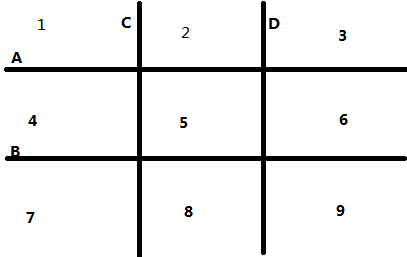
\includegraphics{divi.png}

接下来用$A,B,C,D$与$1 \sim 9$来描述直线与区域。

假如我们$O(9!)$枚举了$b$数列,那么要求$A$上方的点数为$b_1+b_2+b_3$,$B$下方为$b_7+b_8+b_9$,$C$左方与$D$右方也是定值。

如果预处理一个数组来记录$b_1+b_2+b_3=i$时$A$线的可行纵坐标的最大值,那么枚举了$b$数列后一个可行的$A$就出来了。这个预处理是可以$O(n)$的。

而类似的,一个可行的$B,C,D$也能预处理后$O(1)$知道。

容易证明,对于当前枚举的$b$数列,如果这样构造的$A,B,C,D$不合法,那么就没有合法解了,因为他们都只能在一些狭窄的区间内进行摇摆变动,却不能增加或减少哪怕是一个点。我们要做的就是判定合法与否,而合法与否当且仅当$1,3,7,9$四个区域满足题意(因为只要这四个满足题意,则$2,4,6,8$也满足,因此$5$也满足)

那么怎么判断呢?仍然是预处理,我们对于$1$,预处理$A$线纵坐标为$i$时,$C$线横坐标的可行区间。类似的,我们对于$3,7,9$也进行预处理。

预处理的复杂度是多少呢?随着$A$线的下降,$C$线的可行区间只能进行左移,是有单调性的,故$O(n)$。

假如使用基数排序,那么预处理的复杂度就是$O(n)$了,而判断一个解是否合法是$O(1)$的,效率非常高。
\subsubsection{时空复杂度}
时间复杂度:$O(n+9!)$

空间复杂度:$O(n)$
\subsection{Codeforces 248E Piglet's Birthday}
\subsubsection{题意}
有$n$个架子,每个架子有$a_i$个满的蜜罐。

有$m$次操作$u_i,v_i,s_i$,表示从$u_i$个架子上随机拿$s_i$个蜜罐,把这些蜜罐里的蜜都喝光,然后放到$v_i$上。

每次操作之后都要回答所有蜜罐都空了的架子数目的期望值。
\subsubsection{数据范围}
$n \le 10^5$

$0 \le a_i \le 100$

$1 \le m \le 10^5$

$1 \le s_i \le 5$
\subsubsection{题解}
记$prob_{i,j}$为第$i$个架子上有$j$个满蜜罐的概率。

显然答案为$\sum\limits_{i=1}^n prob_{i,0}$

每次操作只会更新一个架子的$prob$,我们只要把这个架子的$prob$算一下就好了。

记函数$F(n,m,k,l)$为$n$个物品,有$m$个特殊物品,我随机选$k$个,正好选中$l$个特殊物品的概率。

记$cnt_i$记录当前操作之前第$i$个架子上的物品数。

把架子$u$上随机选$s$个蜜罐之后,架子$u$有$j$个满蜜罐的概率是$\sum\limits_{k=0}^s prob_{u,j+k}F(cnt_u,j+k,s,k)$。(即枚举随中多少个满蜜罐)

$F$是个很简单的组合数式子,先计算$k=0$的值,然后每次$k+1$时更新一下值,这样复杂度是$O(mas)$的
\subsubsection{时空复杂度}
时间复杂度:$O(mas)$

空间复杂度:$O(na)$
\begin{displaymath}
\end{displaymath}
\subsection{Codeforces 243C Colorado Potato Beetle}
\subsubsection{题意}
你有一个长宽均为$10^{10}+1$的田地。

你在上面画了$n$条线段,线段不会在地图外面。所有被线段经过的格子都会撒上杀虫剂。

虫子从最外层开始入侵,他们无法走到有杀虫剂的格子。

那么求最后没有被破坏的格子数目。
\subsubsection{数据范围}
$n \le 1000$
\subsubsection{题解}
这种题直接统计是不好统计的,但是由于$n \le 1000$,所以我们可以进行模拟。

地图很大,但是离散化后,有意义的点数$O(n^2)$的,我们在新图进行一遍FloodFill也是$O(n^2)$的。

这样问题就顿时变简单了,直接找一个最外面的点开始模拟,统计没有经过的点数就好了。
\subsubsection{时空复杂度}
时间复杂度:$O(n^2)$

空间复杂度:$O(n^2)$
\subsection{Codeforces 266D BerDonalds}
\subsubsection{题意}
一个$n$个点$m$条边无向图,要你找一个点,最小化离他的最远的点到他的距离。

PS:即NOI2013的快餐店那题把环套树改为普通无向图。
\subsubsection{数据范围}
$n \le 200$
\subsubsection{题解}
先用Floyd可以预处理两点间最短路。

枚举每条边进行统计。

沿用NOI那题的思路,我们要找一个类似于直径中点的东西。假设我们枚举边$(u,v)$,认为$p$在边上,那么就是说要找的直径经过边$u,v$。

按离点$u$的距离将其排序,从远至近扫过来,假设扫到的距离为$d$,即确定能通过“$p$走到$u$”的方式走到的点集为距离$u$不超过$d$的,并在扫的时候用一个变量记录剩余点中到$v$的最大值。

也就是说假设$u$所能覆盖的最远点是$a$而$v$能覆盖的是$b$,在合法的前提下$p$取$a,b$中点自然最优。当然要注意$a,b$中点不在边上的情况是不合法的。
\subsubsection{时空复杂度}
时间复杂度:每次枚举边后排序是$O(n^3 \log n)$,如果事先预处理则可以降为$O(n^3)$

空间复杂度:$O(n^2)$
\subsection{Google Code Jam World Final 2011 B Rains Over Atlantis}
\subsubsection{题意}
现在有一个$n \times m$的地图,每个点有海拔高度。

地图的外轮廓是大海。

现在在下非常大的雨,一个点如果四周都比他高,就会积水,直到水可以流入大海。

每个格子的水会向四周海拔最低的那个点流,如果最低的有多个,流向哪里其实是无所谓的。

假设某天格子$S$的水流向了$T$,就会对$S$的土地带来侵蚀,具体的来说,假设点$i$海拔+水深称之为水平面$h_i$,那么$S$的海拔高度会降低$\min(h_S-h_T,M)$,$M$是定值。

求多少天后土地被完全侵蚀。

$T$组数据。

PS:这题略卡题意,如果没看懂建议看详细题面并结合样例理解!(被题意坑的飘过)
\subsubsection{数据范围}
$T \le 10$

$n,m \le 20$

海拔高度与$M \le 10^{15}$
\subsubsection{题解}
首先还是那句话:请看清楚题意。

首先暴力模拟的方法,无非就是每次先用Dijkstra或者SPFA预处理每个点的水平面,然后根据题意来算。当$M$很小而$h$很大时,会有很多时间段的情况是完全一样地。

接下来很容易发现一个性质是说,最多进行$O(n^2m^2)$次的操作后,每个格子的海拔都会以$M$的速度在下降——于是整个时间段可以$O(1)$处理,结束之后会有一个格子被删除。

最多只会有$O(nm)$个格子,每至多$O(n^2m^2)$次后可以$O(1)$计算,问题就解决了。
\subsubsection{时空复杂度}
时间复杂度:$O(SPFA(nm,mm)n^2m^2)$(我是用SPFA写的,而SPFA的复杂度不好说)

空间复杂度:$O(nm)$
\subsection{Codeforces 243E Matrix*}
\subsubsection{题意}
给你一个$n \times n$的01矩阵。你能将列与列任意打乱得到一个新矩阵,使得新矩阵的每一行的1是连续的
\subsubsection{数据范围}
$n \le 500$
\subsubsection{题解}
官方题解是$O(n^3)$的……我不知道具体怎么做。

这题的题意所要求的,其实就是一个数据结构的裸应用——PQ树。

大家可以在2003年的集训度作业里找到相关资料……由于介绍PQ树的资料实在太少,我在此简单讲两句。(建议还是去看相关资料)

PQ树是一个增量构造的树形数据结构,他的性质是按照规定遍历一遍后叶子节点的排列就是一组合法解。

树他的节点分为两种,一种是P类点,一种是Q类点。P类点无特殊性,Q类节点则要求遍历时要么从左往右,要么从右往左。

然后每次就相当于读入一个串后进行增量……我们把要在一起的点标为黑色,一棵子树的叶子节点如果全黑,称为黑子树;全白称为白子树;否则称为灰子树。

如果一个点有超过两个灰子树肯定无解……然后大概思路是说,如果当前是P类节点,你就把一棵灰子树放在左边,后面接着所有的黑子树,然后一棵灰子树放在右边,接下来对灰子树进行递归的操作。注意到他是P类点,所以这样子不能带来改变。你可以新建几个点,让通过让他们向非白点连边以及向白点连边,并让新建点为Q类点,从而达到控制顺序的效果。如果当前是Q类点,要做的则是一个check的任务……

实现中有很多细节问题可能比较恶心……我写的比较逗,用了9K左右的代码。

(最后果然还是没有把PQ树讲清楚……教练求手下留情)
\subsubsection{时空复杂度}
时间复杂度: $O(n^2)$

空间复杂度: $O(n)$
\subsection{Usaco November Contest 2008,toys*}
\subsubsection{题意}
有无限个玩具,你会进行为期$D$天的活动,每天需要提供$T_i$的干净玩具给奶牛玩,奶牛玩过之后即不干净了。

你每天可以选择花$T_c$的代价来买一个干净的玩具。

每个玩具脏了之后可以拿去洗,洗分两种:快洗、慢洗。快洗一件玩具要$N_1$天洗干净,花$C_1$的钱;慢洗一件要$N_2$天洗干净,花$C_2$的钱。

求最小花费以满足要求。
\subsubsection{数据范围}
$n \le 100000$

$T_i \le 50$

$1 \le N_1,N_2 \le D,1 \le C_1,C_2 \le 60$
\subsubsection{题解}
这题的一个经典做法是费用流,曾经出现在湖南省选中(好像叫什么最小餐巾计划之类的东西)。虽然在当时是比较厉害的题,但是现在看来这个做法却是一个非常基础的费用流练习题,建模方式不再赘述。

但是这题和原题的不同之处在于,$n$可以取到$100000$,那么网络流的做法是会TLE的,我们必须得想更优的做法。

有一个非常重要的定理是说,费用流算法,随着流量的增加,费用会是一个凸函数。这个定理我不会证明(我在看黑书白书的时候也没有找到证明),但确实是一个耳熟能详的定理,所以在此我直接引用。

有了这个定理,我们回顾费用流建模,我们会发现最大流恰好是买的玩具的数目!我们可以得到一个结论:花费函数会是关于买的玩具的凸函数。

于是我们可以二分答案,接下来要做的就是已知玩具个数来求最小花费,显然是一个贪心题。我们先不妨默认$N_1 \ge N_2,C_1 \le C_2$,然后一路扫过去,并尽可能的使用慢洗……贪心的正确性比较显然,算法也比较好想。

这题关键在于不仅要能改进传统的网络流做法,还要借助传统做法想到二分答案贪心判定,在我看来这题是一道很好的题目。
\subsubsection{时空复杂度}
时间复杂度:$O(n \log n)$

空间复杂度:$O(n)$
\subsection{Codefroces 266 E,More Queries to Array}
\subsubsection{题意}
要你维护一个大小为$n$的数列,支持以下操作:
\begin{enumerate}
\item 将区间$[l,r]$内的所有值赋值为$x$。
\item 给定$l,r,k$,询问$\sum\limits_{i=l}^r a_i(i-l+1)^k$。
\end{enumerate}
操作数有$m$个。
\subsubsection{数据范围}
$n,m \le 10^5,0 \le k \le 5$
\subsubsection{题解}
虽然说div2不是没有好题……但是div2的数据结构题应该就只有可能是傻逼题了吧……

感觉中国选手一看就会做。将询问的式子用二项式定理展开,我们只要对每个区间$[l,r]$维护$\sum\limits_{i=l}^r a_i(i+1)^k$就好了……直接上线段树。
\subsubsection{时空复杂度}
时间复杂度:$O((n+m) \log nk)$

空间复杂度:$O(n)$
\subsection{Codeforces 338D GCD Table}
\subsubsection{题意}
你有一张$n \times m$的表,第$i$行第$j$列是$(i,j)$,$(i,j)$表示$i,j$的最大公约数。

你有一个大小为$L$的正整数数列$a$,问你是否存在$i,j$,满足对任意$k$,均有$(i,j+k-1)=a_k (1 \le k \le L)$。
\subsubsection{数据范围}
$n,m \le 10^{12}$

$L \le 10^4$
\subsubsection{题解}
首先我们会发现,令$M=lcm(a_1,a_2,a_3,\ldots,a_L)$,$lcm$表示最小公倍数,$i$取$M$的情况下是否有解就代表原问题是否有解了。

我们考虑$j$,会发现等价于要你求$n$个同余方程组的解,第$k$个方程组是$-k+1 \equiv a_k (mod\,M)$。很容易注意到,$j$同样是越小越好,也就是我们求满足同余方程的最小解就行了。

以上都是很好想的……问题关键在于我太逗了,同余方程组竟然只会用中国剩余定理来做,而中国剩余定理又要求互质……后来有人告诉我,黑书上讲了任意两个同余方程组并成一个的方法……嘛,我也不知道那个方法叫什么,反正看上去很基础的样子,就是用扩展欧几里得对两个模方程解出一组解,然后在模他们的最小公倍数意义下就只有这一组解了,然后就能并起来了。

所以就把$L$个方程并起来就没了……所以这题也很水,只是我基础算法不过关。

(有个疑问啊,既然都有了能把任意同余方程组并起来的方法,为什么还要用中国剩余定理这种需要两两互质的算法?中国剩余定理毫无优越性啊)
\subsubsection{时空复杂度}
时间复杂度:$O(n \log n)$

空间复杂度:$O(n)$
\subsection{Codeforces 280D k-Maximum Subsequence Sum*}
\subsubsection{题意}
给你一个大小为$n$数列,要你支持两种操作,操作有$m$个,操作类型如下
\begin{enumerate}
\item 修改某个位置上的值
\item 询问区间$[l,r]$里选出$k$个不相交的子段和的最大值。
\end{enumerate}
\subsubsection{数据范围}
$n,m \le 10^5,k \le 20$
\subsubsection{题解}
这题用线段树做到$O(n \log n k^2)$是很简单的……比赛的时候把这种做法放过去了,其实出题人的做法很厉害,复杂度是$O(n \log n k)$的。

对于如何求$k$段子段和,我们先来看一个搞笑的做法——费用流!

源点向每个点连边,容量为$1$费用为$0$,每个点拆点,$i$向$i'$连边容量为$1$费用为$a_i$,然后$i'$向$i+1$连边……然后限制流量不超过$k$,这样子肯定是对的。

我们来观察这样子的过程,会发现第一次增广,我们会找一个最大的子段和,接下来的增广路要么是再找一个最大子段和,要么是走反边!代价为负的!

线段树可以模拟这个过程!

要支持如下两个操作:查询区间最大子段和与区间整体乘以$-1$,线段树毫无压力。

如此一来,我们用线段树模拟费用流的过程,一次询问最多增广$k$次。
\subsubsection{时空复杂度}
时间复杂度:$O(n \log n k)$

空间复杂度:$O(n)$
\newpage
\section{试题泛做2}
\subsection{Google Code Jam World Final 2014 D Paradox Sort*}
\subsubsection{题意}
$T$组数据。

现有一张竞赛图。

定义函数$f(a,b)$为$a,b$二人中取胜的那一人。

令$S$是个排列,定义函数$f(S)$为$f(f(...f(f(S_1,S_2),S_3)...,S_{n-1}),S_n)$。

求一个最小的排列$S$,使得$f(S)$等于输入的某个定值$x$。或输出无解。
\subsubsection{数据范围}
$n,T \le 100$
\subsubsection{题解}
首先我们来思考这么一个问题:如何判定有无解?

这是个非常有意思的问题。

事实上只要从$x$出发,遍历一遍看是否能遍历到所有点即可。而证明方法则是一个很有意思的构造:按DFS序逆序即可!

有了这个判定方法,问题就好做一些了,我们先按字典序贪心,要做的就是前面已知,并构造后面。判定方法是很简单的,先把前面的点都删了,判定剩余点是否有解,以及剩余点是否有一个能赢前面这些点所得到的点(这个几乎是显然的。假设前面得到的点是$p$,一方面只要有一个点能赢$p$,我们就能让他当$p$的父亲,并按DFS序逆序构造出合法解;另一方面如果没有一个点能赢$p$,最后得到的也只能是$p$而不会是$x$。当然$p=x$要特殊处理)。
\subsubsection{时空复杂度}
时间复杂度:$O(TN^4)$。(几乎卡不到上界)

空间复杂度:$O(n^2)$
\subsection{USACO December Contest 2012, Gangs of Istanbull/Cowstantinople}
\subsubsection{题意}
有$m$个帮派,每个帮派有$s_i$头牛。总共有$n$头牛。

现在$n$头牛要依次进入牧场。一头牛进入牧场后,如果牧场没有牛或者牧场里的牛和他同帮派,不会有影响;否则的话,他会和牧场上的一头牛争吵,并两人一起离开。

如果牧场上有牛,就称之为这头牛所属帮派控制了牧场。

求帮派1能否控制牧场;如果能最后最多剩下几头牛;在满足前两问最优的情况下输出字典序最小解。
\subsubsection{数据范围}
$n \le 10^6$

$1 \le m \le n$
\subsubsection{题解}
先考虑前两问,我们的想法是让帮派$2 \sim n$的人拼命打架,看最后能剩下几个。

这是经典问题,答案是如果最大值超过总量一半,就让所有人去和最大值打架;否则如果总量是奇数,就可以只留下一个;否则就一个数都不会留下。

事实上这个性质也是能帮助字典序上的贪心的。

贪心过程可能略复杂,基本上就是利用那个经典问题的答案,一路扫过去就好了。把帮派1先预留出答案头牛。每次找到最小的还有牛的帮派,让他里面所有的牛都进牧场,然后在后面的帮派中来找牛与他进行两两抵消。为了时刻保证有解,我们只需要维护好“当前最大值和总量”这两个变量就行了,总量只要在实现过程中处理一下就好了,最大值用个桶来维护。
\subsubsection{时空复杂度}
时间复杂度:$O(n)$

空间复杂度:$O(n)$
\subsection{Codeforces 311C The Great Julya Calendar*}
\subsubsection{题意}
你可以对一个数$n$进行变换,变换方式是把这个数减去他十进制意义下的某个数位上的数。

要用最少的次数把它变成0。

比如 24->18->10->9->0。
\subsubsection{数据范围}
$n \le 10^{18}$
\subsubsection{题解}
显然能得到贪心结论:每次减去能减的最大值(因为这是个单调递增函数)。

考虑数位dp。

$dp[n][i][j]$表示末尾的$i$位是$n$,然后$i$位之前的这些位的最大值是$j$,第一次小于等于$0$的最少步数。

至于转移的话,假设$n'$是贪心操作后使第$i$位第一次减少了$1$时得到的数字(这当中花了$t$步)。

那么$dp[n][i][j]=dp[n'][i][j]+t$。

而$t$等于多少?若$n$的后$i-1$位是$x$,第$i$位是$y$,$t=dp[x][i-1][max(y,j)]$。

状态数是非常少的,是$\log$级别。用hash表或者map存下来就好了。
\subsubsection{时空复杂度}
时间复杂度:$O(\log^2 n)$或者$O(\log n)$(视是否使用map而定)

空间复杂度:$O(\log n)$
\subsection{Codeforces 268D Wall Bars}
\subsubsection{题意}

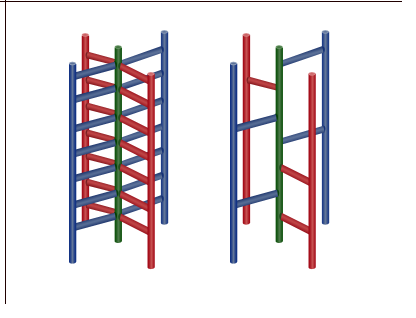
\includegraphics{wall.png}

有一种娱乐设施叫做Wall Bar,他由五根柱子形成,柱子长为$n$。周围的四根会向中间连横杠,如左图是连满的样子。

现在改变规则,对于每个高度,你只能从中心柱子连出一条横杠向某个柱子,如右图。

一个小朋友来玩,他刚开始在地面上,可以认为高度为$0$。每次,他都能选择一个高度不比他大$h$的当前柱子上的横杠,爬上去。特别的,在地面上时则可以在周围四个柱子里任意选择一个柱子上的高度不超过$h$的横杠。

问有多少种合法的建造方法,使得小朋友能爬到最上面。
\subsubsection{数据范围}
$n \le 1000$

$h \le min(30,n)$
\subsubsection{题解}
由于$h$很小,又只有$4$根柱子,我们不妨把每根柱子离自己的距离给设入状态。

即$f(i,a,b,c,d)$表示到了高度为$i$,四根柱子与自己的距离分别为$min(h+1,a),min(h+1,b),min(h+1,c),min(h+1,d)$。

如果某个时刻距离达到了$h+1$,就恒为$h+1$。

转移显然,来考虑状态数?

首先,我们可以对$a,b,c,d$用最小表示,如此就是$O({h \choose 4})$。

然而,注意到“当前踩到”的这个位置,对应的距离要么是$0$,要么是$h+1$。于是这样的状态数就是$O(h^3)$了。

当然再深入思考,最小表示仍然是可以用的,于是状态数就是$O({h \choose 3})$。

这样问题就解决了。空间问题能用滚动数组优化。
\subsubsection{时空复杂度}
时间复杂度:$O(n {h \choose 3})$

空间复杂度:$O(h^3)$
\subsection{Codeforces 286D tourist}
\subsubsection{题意}
在某些时刻$q_i$,会有两个人分别从$(-1,0)$与$(1,0)$竖直向上以每秒移动单位长度1的速度行走。

在某些时刻$t_i$,会在点$(0,l_i)$与点$(0,r_i)$间瞬间出现一堵墙。

对于每对人,求他们相互能看得见的时间。

总共有$n$个墙出现;总共有$m$对人。
\subsubsection{数据范围}
$n,m \le 10^5$

$l_i,r_i,t_i,q_i \le 10^9$
\subsubsection{题解}
离散化后,总共有$O(n)$个线段。每个线段只要知道第一次有墙覆盖他的时刻就行了。于是我们把题目可以看做有$O(n)$个互不相交的墙在某些时刻瞬间出现。

如何处理处离散化后的每个线段的出现时间?这可以用简单的线段树在$O(n \log n)$的时间里实现,同时也能用并查集或者平衡树(只需要set即可)分别在$O(n\alpha(n))$与$O(n \log n)$的时间复杂度更加简单的求出。具体思想就是每次找一个没有被覆盖的进行覆盖,只会有$O(n)$次有效操作。

对于一面墙,可以算出他的两个参数$L,R$,理解为若出发时间小于$L$,无影响;若出发时间在$[L,R]$里,影响是个一次函数;若出发时间大于$R$,影响为墙的长度。

对时间也离散化后就只有$O(n)$个有效时间,我们维护一次函数相当于维护两个数组(分别是$y=kx+b$的$k$与$b$),对这两个数组都是支持区间加单点查询的操作。很显然我们只要用一个差分数组就能$O(n)$处理。

所以这题就没了……感觉顺着题目该维护什么就维护什么就行了,没什么要绕弯的地方,只要熟练这些技巧就行了。
\subsubsection{时空复杂度}
时间复杂度:$O(n \log n)$

空间复杂度:$O(n)$
\subsection{Codeforces 360D Levko and Sets}
有两个整数数组$a_1,a_2,...,a_n$与$b_1,b_2,...,b_m$与一个质数$p$,现在他生成了$n$个集合,第$i$个集合的生成方式如下:

\begin{enumerate}
\item 开始,集合只有元素$1$。
\item 我们从集合里选出一个元素$c$,对于所有的$j$,如果满足$c\times a_i^{b_j} \mod p$不在当前集合,就把它加入集合。
\item 重复以上步骤。
\end{enumerate}

求$n$个集合的并的大小。
\subsubsection{数据范围}
$n \le 10^4,m \le 10^5,b_i \le 10^9,p \le 10^9,a_i < p$

保证$p$是质数。
\subsubsection{题解}
原根拼命上!

首先素数都有原根,求素数原根的复杂度是能过的。

然后是原根可以很方便的把一个数变成$g^s$,于是在以$g$为底的对数意义下,乘法就转变为加法了。

利用大步小步可以对每个数都取$\log$,设$g^{c_i}=a_i$,那么根据裴蜀定理,令$x=gcd(c_1,c_2,c_3,...,a_n,p-1)$,能表示出来的数字,就是$g^{kx}$。

此处分块大小可以调一下,从而保证复杂度(因为预处理只用一次,查询要很多次)。比如我强行$10^6$个数字一块。

这么一来,就是说有一个数集,求$[0,p-1]$中有多少个数能被这个数集中的至少一个数整除。

显然能用容斥原理计算,对于每个出现在给定数集的$p-1$的因数$x$,设$dp[x]$表示能被$x$整除又不能被$x$的出现在数集中的倍数整除的数有几个。直接暴力约数平方的计算就好了。
\subsubsection{时空复杂度}
时间复杂度:$O(na_i/10^6+\gamma^2(p-1))$,$\gamma(n)$表示$n$的约数个数。

空间复杂度:$O(n+10^6)$
\subsection{Codeforces 316G3 Good Substrings}
\subsubsection{题意}
我们用一个三元组$(p,l,r)$表示一个规则,其中$p$是个字符串,$l,r(l \le r)$是整数。我们说字符串$t$满足规则$(p,l,r)$,当且仅当字符串$t$在$p$中的出现次数在$[l,r]$内。

我们说一个字符串是好的当且仅当满足所有的$n$个规则。要你求一个字符串$s$中的好的子串个数。
\subsubsection{数据范围}
$0 \le n \le 10$
字符串$s$和$p_i$的串长均不超过$50000$
\subsubsection{题解}
先将所有串都插入一个后缀数组,如此一来,我们就能用ST表二分从而在$O(\log n)$的时间里询问一个串出现了几次。

对于每个左端点$i$,对应的右端点$j$的可行区域是一段区间。考虑如何求这个区间。

对于左端点$i$和每个规则,我们都可以求出一个区间使得以$i$为左端点以区间为右端点的串符合规则。

注意到随着$i$的增加,对应的区间一定是往右边移动的(因为字符串长度变小了出现次数就一定会变多,长度变长出现次数一定会变少),我们就不需要每次二分来做,只需要利用单调性扫即可,移动的次数一定是线性的。

于是这题就解决了,复杂度也只有一个$\log$,不过用后缀自动机应该能整个线性……
\subsubsection{时空复杂度}
时间复杂度:$O(nL \log L)$,$L$代表串长。

空间复杂度:$O(nL)$
\subsection{Google Code Jam World Final 2014 E Allergy Testing*}
\subsubsection{题意}
现有$n$种食物,你会对当中恰好一种食物过敏。

你每次操作可以选择若干个食物吃掉,$A$天之后会知道是否过敏,如果过敏,你需要再等$B-A$天身体才会好转(也就是说不过敏会花费$A$天,过敏会花费$B$天)。

要你用最少的天数,试出让自己过敏的食物。

$T$组数据。
\subsubsection{数据范围}
$1\le n \le 10^{15},1 \le A \le B \le 10^{12},1 \le T \le 10$
\subsubsection{题解}
此题是神题。

由于直接做不好做,我们考虑二分答案转化为判定问题,即判定$n$天所能得到的最多的食物数目。

对于$50\%$的数据,我们可以用动规的方式思考问题。可以得到动规方程为:

\begin{eqnarray*}
f(n) =
\begin{cases}
1 & n \le A-1 \\
f(n-A)+1 & A \le n \le B-1 \\
f(n-A)+f(n-B) & B \le n
\end{cases}
\end{eqnarray*}
第一、二种情况是显然的;第三个式子则比较有意思,但很遗憾$50\%$的做法与满分做法关系不大,这里留给读者自己思考。

对于满分,我们这么来想:

假如$n$个食物,无论哪个食物有问题,都可以用$T$天判定出来,那说明了什么?

假如我们已经有了一种决策——即先吃某些食物,如果过敏选择一个子状态,不过敏选择另一个子状态,最后无论过敏的是哪个食物,我们都能判定,这可以用一个博弈树的模型来刻画。

初始集合是全集,可以看做根,我按照最优决策取一些吃,可以理解为若不过敏就走做儿子状态,否则走右儿子状态。如果走到了叶节点,就代表判定成功。走到一个点需要代价,这些代价就是这个决策过程中的天数。

用这个模型思考,就相当于我们要构造一棵博弈树,满足根到任意一个点的代价不超过二分的上限$T$的情况下,最大化叶子个数。

从根走到一个点可以看做向左走了$X$次,向右走了$Y$次,来计算代价的话问题却出现了:如果最后一步是左儿子,我们花费$AX+BY$的代价;如果是右儿子,我要花费$A(X+1)+B(Y-1)$的代价,这是很不方便的。

我们让父节点来分担一些右儿子结尾情况的贡献,会得到结论:一个向左走$X$向右走$Y$的点为叶子,当且仅当$T-B < AX+BY \le T$。

是否觉得有点突然,我们来详细的分情况讨论一下:
\begin{enumerate}
\item 对于最后一步是向左儿子走的情况,花费是$AX+BY$。他不能再往左儿子走了,于是有$T-A < AX+BY \le T$,这是“最后一步是朝左边走”的充要条件。
\item 对于最后一步是向右儿子走的情况,花费是$A(X+1)+B(Y-1)$,应该有$T-A < A(X+1)+B(Y-1) \le T$而他父亲的花费则是$AX+B(Y-1)$。那么在区间$(T-B,T]$内,他与他父亲至多只会有一个出现!如果要详细的分情况讨论,应该是若$T-B < AX+BY \le T$,则父亲$AX+B(Y-1)$一定会小于或等于$T-B$;反之若$AX+BY > T,T-B < A(X+1)+B(Y-1) \le T$,那么他父亲就会带来贡献:$T-B < AX+B(Y-1) \le T$
\end{enumerate}

分析到了这一步,也就差不多了。如果已知向左走$X$步,向右走$Y$步,很容易知道这样的方案数是${{X+Y} \choose {X}}$我们要求的是
\begin{displaymath}
\sum_{X} \sum_{Y} {{X+Y} \choose {X}} [T-B < AX+BY \le T]
\end{displaymath}

我们可以随手构造一个博弈树:每次把$n$平分一半,弄一棵完全二叉树。这样子的代价不会超过$B \log n+A$,于是我们知道,$f(T)\ge n$的$T$是不会超过$B \log n+A$的,于是我们的$Y$就最多只用枚举到$\log n$即可。

如果我们枚举了$Y$,就可以$O(1)$算出$X$的上下界,用前缀和思想一减,要求的就是一个形如$\sum_{i=1}^m {{n+i} \choose {i}}$的式子,稍微了解一点组合数的恒等式,就知道这个式子等于${{n+m+1} \choose {m+1}}$

我们要判断的是一些东西加加减减是否超过$n$,用高精度当然可以,但事实上不用这么麻烦,我们用取对数的方法可以判断一个组合数与$n$的大小关系,利用一些放缩法的技巧,是可以避免高精度的。当然由于这题数据范围不大,即使写了高精度也没关系。

问题至此解决了。
\subsubsection{时空复杂度}
时间复杂度:$O(T\log^2 n)$

空间复杂度:$O(1)$
\subsection{Codeforces 325C Monsters and Diamonds}
\subsubsection{题意}
有$n$种怪物,每种怪物都有一个$1 \sim n$的唯一编号。

现在有$m$个规则,每个规则代表将某个怪物分裂成一些东西(指的是将一个怪物分裂成若干个怪物与若干个钻石)。

求你解决完所有怪物的前提下,能得到的钻石的最小值和最大值。
\subsubsection{数据范围}
$n,m \le 10^5$

分裂出的物品总和不会超过$10^5$
\subsubsection{题解}
首先我们先来看最小值该如何求。

这是个很常考的问题,在JSOI中和以前的清华集训和其余的CF比赛中都出现过(为什么考的这么多啊?),首先用SPFA暴力迭代肯定是可以的,也可以用堆优化Dijkstra来做,只要加上一句话:一个点入队的前提是他会分裂到的所有点都已经入队过了。

那么最大值怎么求呢?最大值是不能暴力迭代的,但是我们可以考虑用记忆化搜索的方式来$dp$。

记忆化搜索,一条环就是无穷大,同时因为算出了最小值,我们能够分辨出一个点究竟能不能分裂完。

在保证只会走到能分裂完的点的前提下,记忆化搜索,对于环就表示无穷大,这样子就能解决最大值了。
\subsubsection{时空复杂度}
时间复杂度:$O(n \log n)$(如果用的是堆优化Dijkstra的话)

空间复杂度:$O(n)$
\subsection{USACO December Contest 2012, First!}
\subsubsection{题意}
现有$n$个字符串,你能任意改变字母表的顺序从而达到改变字典序的效果。

求哪些字符串存在一种方式让它变成字典序最小的字符串。
\subsubsection{数据范围}
$n \le 30000$

记字符串总长为$L$,有$L \le 300000$

字符串互不相同
\subsubsection{题解}
显然地,我们可以先将它们都插入一棵trie中。

如果强制要求某个串最小,那么顺着他在trie中对应的链走下去,对于链上的每个节点对应的字符,都要求比其他所有兄弟小,这样子会有不超过$26\times l_i$个约束条件,$l_i$表示第$i$个字符串的长度。每个约束条件都是形如“某个字符的位置比某个字符的位置小”的形式。

最后要做的是判定这些约束条件下是否有解。判定是很简单的,可以看做是要求一个$26$个点的拓扑序,然后要求某些点一定在某些点前面。

我们只要对于约束条件“$u$在$v$之前”,连一条$u$到$v$的有向边,最后判断这个拓扑图是否有环即可。
\subsubsection{时空复杂度}
时间复杂度:$O(26^2n+26L)$

空间复杂度:$O(26L)$
\subsection{Codeforces 269 E String Theory*}
\subsubsection{题意}
有一架$n$行$m$列的长方形竖琴,上下边界处均匀的有$m$个钉子,左右边界处均匀的有$n$个钉子。

总共有$n+m$个琴弦,每一根琴弦两端被钉子固定在竖琴不同侧的边界上,而且每个钉子上有且仅有一根琴弦。

他认为如果有琴弦相交,这个竖琴就无法弹奏。

你能对琴弦进行一种变化,变化方式如下:
\begin{enumerate}
\item 选择不同的两列,对应地交换处于同侧的钉子(两侧必须同时交换),但不改变钉子与其所固定的琴弦的连接;
\item 选择不同的两行,对应地交换处于同侧的钉子(两侧必须同时交换),但不改变钉子与其所固定的琴弦的连接;
\end{enumerate}

比如

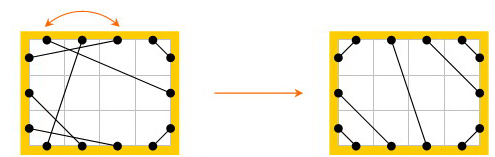
\includegraphics{string.png}

现在要求你用一种变化方式,使得没有琴弦相交,如果有解输出任意一组,否则输出无解。
\subsubsection{数据范围}
$n,m \le 10^5$
\subsubsection{题解}
首先问题的关键在于,最终形态唯一确定。

对于左边连向上边的,一定得是左边第一个连向上边第一个,否则必然造成相交。以此类推,左边连向上边的琴弦位置是固定的。

对于左边连向下边的和左边连向右边的,一定先让左边连向右边再让左边连向下边,以此类推,左边的琴弦都是固定的。

同理,下边连向上边的一定在下边连向右边的之前。

于是所有琴弦位置固定,可以看一个例子。

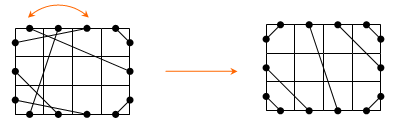
\includegraphics{string_sample.png}

左边的要想合法,根据上面的推理,只能变成右边这样子。

我们从一个点出发,走到琴弦的另一端,然后走到与他面对面的点,再走到琴弦的另一端,再走到面对面的点,再走到琴弦的另一端……最后会形成一个环。

每次取出一个不在环上的的点,把他所在的环抓出来。

如此会将一个竖琴看做若干个环,每次操作只会对一个环进行轮换操作!

我们把一个环上每个点所在的边界类型(即"UDLR")给写下来表示一个环。

我们称环$A$与环$B$等价当且仅当环$A$是环$B$的一种循环表示,或者如果环$A$的某个循环表示翻转后能得到环$B$。(后面这个容易漏想)

我们称竖琴$A$与竖琴$B$等价当且仅当竖琴$A$的环数与竖琴$B$的环数相等,并且能找到一组完备匹配使得竖琴$A$的每个环都与竖琴$B$的某个环等价。

可以证明你能将某个环变成他的一个等价环;如此一来只要输入竖琴与能得到的那个竖琴等价就有解,反之就无解。

判定是否等价我用的是hash,即先对每个环翻转并接在后面(如此可以解决翻转同构的问题),然后求最小表示串,将最小表示串hash,然后对每个环的最小表示串hash值排序。

竖琴$A$与竖琴$B$等价就是对应的各个环的最小表示串hash值排序后的数列相等。

输出解就只要把环一个个匹配,对每个环分别把它们变换成相等就行了。也就是对两个环分别求最小表示,然后各自最小表示对应的点连成琴弦。
\subsubsection{时空复杂度}
时间复杂度:$O(n \log n)$

空间复杂度:$O(n)$
\subsection{Codeforces 323C Two permutations}
\subsubsection{题意}
你有两个各包含n个元素的排列$p$和$q$,和$m$个由$l_1,r_1,l_2,r_2$组成的询问。每次询问在$p$中位置在$[l_1,r_1]$,在$q$中位置在$[l_2,r_2]$中的数的数量。

强制在线。
\subsubsection{数据范围}
$n \le 10^6$

$m \le 200000$
\subsubsection{题解}
对于每个数,记他在$p$中的位置是$x$,在$q$中的位置是$y$,我们就相当于抽象为平面上有$n$个点。

而对于一组询问,就相当于询问一个矩形内有多少点。

于是问题抽象为平面上有$n$个点和$m$个矩形,要问每个矩形内有几个点,强制在线,复杂度要求在$O((n+m) \log n)$内。

这是非常经典的主席树应用,直接得到横坐标在$[1,i]$的所有点形成的线段树后就能用前缀和思想做了。
\subsubsection{时空复杂度}
时间复杂度:$O((n+m) \log n)$

空间复杂度:$O(n \log n)$
\subsection{Codeforces 254D Rats}
\subsubsection{题意}
一个地图,里面有一些老鼠。为了清除老鼠,某人选择丢两个手榴弹。

地图是$n \times m$的网格图,里面有些位置有墙,其余位置是空的。有些位置有老鼠,老鼠们睡着了不会动。

你只能在没有墙地方放炸弹,每秒钟,炸弹的波及范围会延伸一格,但是炸弹的延伸过程是不会波及到墙的,一个简单的例子如下图:

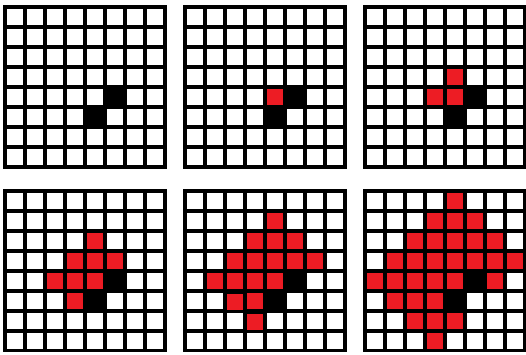
\includegraphics{rats.png}

黑色代表墙壁,第二幅图的红点代表炸弹放置为止,接下来每张图代表下一秒钟的情况。

炸弹在爆炸$d$秒后会瞬间消失。

问是否能找到两个格子放置炸弹,使得炸死所有老鼠。
\subsubsection{数据范围}
$n,m \le 1000$

$d \le 8$
\subsubsection{题解}
$n,m$很大,我们不能枚举所有点。

突破口在于$d$很小,所以炸弹离老鼠必须很近,于是炸弹的可行位置就有限了。

先看第一只老鼠,由于必须有炸弹炸死他,所以炸弹是到他的最短路不超过$d$的点集(最多只有$O(d^2)$个)。

暴力枚举能炸死第一只老鼠的炸弹的位置,接下来找到一个没有被炸死的老鼠,再在他附近的$O(d^2)$个位置枚举第二个炸弹。

枚举完之后判定是否炸死所有老鼠即可。
\subsubsection{时空复杂度}
时间复杂度:$O(d^6+nm)$

空间复杂度:$O(nm)$
\subsection{Codeforces 243D Cubes}
\subsubsection{题意}
现在有一个$n\times n$的网格,每个格子上面放有$a_{i,j}$个立方体。现在有无数方向向量为$(sx,sy,0)$的平行光束从无穷远处射来,求能看到的立方体数目。

PS:一个立方体能被看到,当且仅当上面存在一个点,往向量$(-sx,-sy,0)$处看去,一直到无穷远处中间没有任何立方体阻挡
\subsubsection{数据范围}
$n \le 1000$

$|vx|,|vy| \le 10^4,|vx|+|vy|>0$

$0\le a_{i,j} \le 10^9$
\subsubsection{题解}
由于向量第三维是$0$,显然可以在平面上思考问题。

一开始想歪了,往$gcd$方面去想,其实$gcd$只是处理点的,不好扩展到正方形上。

我们来考虑一个正方形遮挡的形状以及一个正方形是否被遮挡的判定,由于直接做不好做,可以将其进行投影。

换句话说,我们沿平行光将其投影到y轴,此时容易证明一个点能不能被看到等价于这个点的投影是否被别的他反方向的正方体的投影覆盖。类似的,一个正方形是否能看到也就是正方形所投影成的线段,会不会被别的线段完全覆盖掉。

那么如何更方便的来看两个正方形谁在谁的反方向呢?相信你已经发现,这个距离能用点积刻画。

换句话说,我们把所有正方形按点积排序,依次考虑,每次来看覆盖这个正方形的投影线段上的最矮点,更新答案,并拿他的高度更新这个正方形的投影线段。

既然是线段,我们当然就用线段树来维护。离散化后,要做的就是查询区间最小值,以及让一个区间的所有值与某个值取$max$,这是很简单的线段树操作。
\subsubsection{时空复杂度}
时间复杂度:$O(n^2 \log n)$

空间复杂度:$O(n^2)$
\subsection{Codeforces 283E Cow Tennis Tournament}
\subsubsection{题意}
有$n$头奶牛,每两个奶牛有个武力值$a_i$,他们两两间会有比赛。

武力值互不相同,刚开始时两头奶牛比赛的胜负性完全由武力值高低决定。于是有$m$个操作,每次操作为把一段区间里任意两人的胜负关系取反。

最后要你求有多少三元组$(a,b,c)$满足$a$胜$b$,$b$胜$c$,$c$胜$a$。
\subsubsection{数据范围}
$n,m \le 10^5$

$a_i \le 10^9$
\subsubsection{题解}
利用补集转化的思想处理三元环是非常经典与古老的,具体来说,我们求第$i$个点赢得场数为$d_i$,那么拿${n \choose 3}$减去$\sum\limits_{i=1}^n d_i(d_i-1)/2$就是答案,由于模型过于经典(可以在白书第二章的介绍知识的模块看到),在此略去其原理。

知道了这个技巧,我们要做的就是对每头牛,求他胜利的场数。

排序后重编号,正常情况下,每个牛是赢他左边的所有牛,输他右边的所有牛。

我们思考能不能做这样的事情:枚举每个牛$i$,对于任意的牛$j$,如果他们的胜负关系改变,就标记为$1$,否则标记为$0$。如果能做,对于每个牛,就是统计左边的$0$与右边的$1$有多少个。

用离线很容易处理,我们用类似于扫描线的思想,一路扫过去,进行如下流程:
\begin{enumerate}
\item 扫到第$i$个点时,把所有以$i$为左端点的修改区间拿出来,将这些区间对应的做一次区间的$0,1$反转操作。
\item 统计第$i$个点左边的$0$与右边的$1$,这就是第$i$个点的胜利场数。
\item 将所有以$i$为右端点的修改区间拿出来,将这些区间的贡献进行“撤销”,即将对应区间再做一次区间的$0,1$反转操作。
\end{enumerate}

如此即可,这是一种非常有效的离线技巧,他能方便的做到对于每个点,只有覆盖了他的区间才会对答案带来贡献。
\subsubsection{时空复杂度}
时间复杂度:$O(n \log n)$

空间复杂度:$O(n)$
\newpage
\section{试题泛做3}
\subsection{Codeforces 339E Three Swaps}
\subsubsection{题意}
给你一个排列$a_1,a_2,\ldots,a_n$,你可以执行翻转操作,即每次将一段区间$[l,r]$的数进行翻转。

要你用不超过$3$步,将一个$1,2,3,\ldots,n$的排列变成排列$a$。

\textbf{保证有解}。
\subsubsection{数据范围}
$n \le 1000$
\subsubsection{题解}
我们可以加上一个限制条件:每次翻转$[i,j]$时,必须要求$|a_i-a_{j+1}|=1$或者$|a_j-a_{i-1}|=1$。令$a_0=0,a_{n+1}=n+1$。

加上这个限制条件的正确性在操作$1,2$步时是显然成立的,而在$3$步并不显然,因为存在不满足这个条件却能成功翻转的例子,但那个例子却有满足这个条件的方案。

如果按区间的位置关系进行分情况讨论的话,$3$步之内应该也是正确的。

至于时间复杂度的问题,由于保证有解,$3$步顶多只会让原数列分成不超过$7$段,段的定义是相邻位置相差$1$。这样的话段数可以看做一个不大的常数。
\subsubsection{时空复杂度}
时间复杂度:$O(n^2)$

空间复杂度:$O(n)$
\subsection{Codeforces 309D Tennis Rackets}
\subsubsection{题意}
你需要设计一个网球拍。

有一个正三角形,每条边上有$n$个小孔,你要在小孔上穿线。最近的$m$个小孔是通风口,不能穿线。

一个球拍需要在三条边上各选一个非通风口的小孔,连接成一个三角形,要求三角形式钝角三角形,如下图:

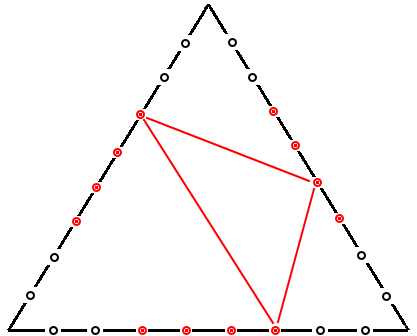
\includegraphics{tennis.png}

求方案数。球拍等价当且仅当某一个点选的不同(即不考虑翻转同构)
\subsubsection{数据范围}
$n \le 30000$
\subsubsection{题解}
如果枚举了点$A,B$,$C$显然是有单调性的。

这么做就是$O(n^2)$的,感觉没有什么优化的思路。

所以正解就是卡常数了。

(又是一道无聊题)
\subsubsection{时空复杂度}
时间复杂度:$O(n^2)$

空间复杂度:$O(n)$
\subsection{Codeforces 249D Donkey and Stars}
\subsubsection{题意}
给你平面上$n$个点,一个点能看到的范围,可以理解为从他射出两条射线,与$x$轴的夹角分别是$\alpha_1,\alpha_2$。他能看到射线夹住的范围,如图:

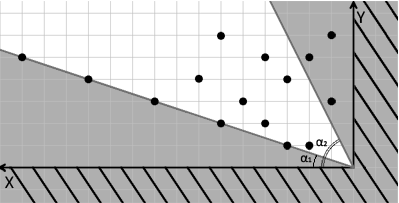
\includegraphics{stars1.png}

要求你从原点出发,找到一个能看到的点,走到这个点上再找一个能看到的点……可以结合这么一个例子:

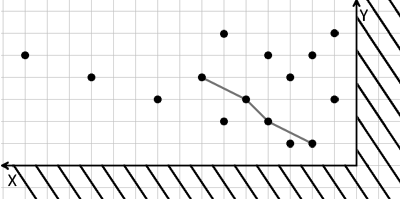
\includegraphics{stars2.png}

要求使得过程中的点最多。

也就是找一个序列,使得序列的每个点(除了最后一个点),都能看到他的后一个点,序列第一个点是原点,要求让序列最长。
\subsubsection{数据范围}
$n \le  10^5$
\subsubsection{题解}
我们来考虑一个点$A$能看到另一个点的$B$情况。

首先,要求$A$离原点更近,这是显然的。

其次,取两个向量$\overrightarrow{v_1},\overrightarrow{v_2}$,分别满足表示射出去的两条射线,要求$\overrightarrow{AB} \times \overrightarrow{v_1}>0,\overrightarrow{AB} \times \overrightarrow{v_2}<0$

把式子一些,最后会发现可以转化为这么一个问题:$A$可以用三元组$(x_1,y_1,z_1)$表示,$B$可以用三元组$(x_2,y_2,z_2)$表示,$A$能看到$B$当且仅当$x_1<x_2,y_1<y_2,z_1<z_2$。

这是经典的三维偏序问题,我用树状数组套线段树过掉了。
\subsubsection{时空复杂度}
时间复杂度:$O(n \log^2 n)$

空间复杂度:$O(n \log^2 n)$
\subsection{Google Code Jam World Final 2009 F Lights}
\subsubsection{题意}
有两个光源,一个发红光,一个发绿光。

有$n$个圆是,他能吸收光线。

有些区域没有光线到达,是黑色的。

有些区域只有红光到达,是红色的。

有些区域只有绿光到达,是绿色的。

还有些区域既有红光到达也有绿光到达,是黄色的。

求四种颜色的面积。
\subsubsection{数据范围}
$n \le 50$

$x,y \le 100$
\subsubsection{题解}
$x,y$很小,又是求面积,这提醒我们使用辛普森算法。

于是要做的就是在$x=k$这么一条竖线上做区间覆盖问题。

但是找区间却是非常非常恶心的,细节繁杂,以至于我写了4.5K的代码。

为了避免辛普森的误差,我们能够分成$100$段,对每一段进行计算。
\subsubsection{时空复杂度}
时间复杂度:$O(100n\times Simpson)$,$Simpson$代表辛普森算法的运行次数。

空间复杂度:$O(n)$
\subsection{Codeforces 238E Meeting Her}
\subsubsection{题意}
有$n$个城市,$m$条有向边,起点在点$a$,终点在点$b$,Urpal要从起点到终点去。

Urpal想做公共汽车。总共有$k$个公车公司,每秒钟,第$i$个公车公司都会有一辆车随机选择一条$s_i$到$t_i$的最短路(如果没有$s_i$到$t_i$的路径的话这个公司就不会有车)。如果车经过了Urpal所在点,他就能上车,并在任意位置下车。

他想知道最坏情况下他要换几次车到终点,如果最坏情况下不能到就输出-1。
\subsubsection{数据范围}
$n,k \le 100$
\subsubsection{题解}
这种题因为转移有环,所以一般都是迭代。

首先Floyd预处理出任意两点最短路,以及预处理出某点走到某点的第$i$步的可能到达点集合。

令$dp[i]$表示从$i$出发的答案。

暴力迭代,每次枚举每个公司,如果公司有个必须经过的点$x$,就能更新$x$的答案,更新方法大概是计算一个$g$数组,表示坐上这辆车的最坏情况下的最小次数。

$g$是很容易转移的,求出$g$就能求$dp$了。
迭代次数至多不超过$n$次。迭代一次的复杂度是不超过$O(kn^2)$的。
\subsubsection{时空复杂度}
时间复杂度:$O(n^3k)$

空间复杂度:$O(n^2)$
\subsection{USACO Open Contest 2014, Code Breaking}
\subsubsection{题意}
有一棵$n$个点的有根树,每个点都要写个$0 \sim 9$的数字。

给你$m$个约束条件,形如$p_i,s_i$,表示对于将$p_i$以及$p_i$的四级祖先这五个点的数字接起来,不能是$s_i$。

求方案数对$1234567$取模。
\subsubsection{数据范围}
$n \le 20000,m \le 50000$
\subsubsection{题解}
一个$O(10^5 n)$的做法是暴力$dp$,记$dp[i][j]$为以$i$为根的子树,$i$的四级祖先到$i$的数字是$j$的方案数。

而一个优化是不记自己,这样子是$O(10^4 n)$的。

考虑优化这个算法,我们发现假设有约束条件$x,11111$,那么对于$x$而言,四级祖先是$0,2,3,4,\ldots,9$是一样的。

换句话说,我们开$n$个trie,对于一个约束条件$x,s$把$s$的所有后缀插入$x$的trie,把$s$的前四位的所有后缀插入$x$的父亲的trie,以此类推。

即设$dp[i][j]$为以$i$为根的子树,然后他的四级祖先的串在他的trie上跑一边会返回$j$,这种情况下的方案数。

状态数是$O(n+m)$级别的。

转移需要枚举他的所有子树,暴力转移是$O(\sum\limits_{i=1}^n d_is_i)$,$d_i$表示度数,$s_i$表示$i$的trie上的节点数。

用一棵菊花树可以让算法退化。

考虑用数据结构优化,观察$dp$方程,会发现是求一些东西的乘积,支持单点修改。

由于模数是合数,不能用树状数组(当然你可以对他的质因子分别作然后中国剩余定理合并),我们能使用线段树实现。
\subsubsection{时空复杂度}
时间复杂度:$O((n+m)\log n)$

空间复杂度:$O(n+m)$
\subsection{Codeforces 280E Sequence Transformation*}
\subsubsection{题意}
给你一个非减的序列$x_1,x_2,\ldots,x_n(1 \le x_1 \le x_2 \le \ldots \le x_n \le q)$。你还有两个整数$a$和$b(a \le b,a(n-1)<q)$。

你要把序列变成$y_1,y_2,\ldots,y_n(1 \le y_i \le q,a \le y_{i+1}-y_i \le b)$。

变换的代价为$\sum\limits_{i=1}^n (x_i-y_i)^2$。

最小化变换代价。
\subsubsection{数据范围}
$n \le 10^5$
\subsubsection{题解}
这是一场中国人出的比赛的E题。

是一道CTSC题目的加强版。

设$dp[i][x]$为前$i$个数,最后一个数变成$x$的最小代价。

$dp[i][x]=\min(dp[i-1][y])+(x-a_i)^2$,要求$x-b \le y \le x-a$。

当然这个$dp$是没法用循环做到的,因为$x$是实数。

我们不妨想像成$dp[i]$是个函数。

首先一个结论是说,$dp[i]$是个凸函数。

证明很简单。我们需要证明的是$dp[i]''>0$。用数学归纳法。

对于$dp[1]''$,显然等于$2$。

若$dp[i-1]$是凸函数,$dp[i]$应该是这么得到的:

假设$dp[i-1]$的极值点是$(x,dp[i-1][x])$,那么我们在$[x+a,x+b]$处画一条平行于$x$轴的纵坐标为$dp[i-1][x]$的线段,然后将$dp[i-1]$于$x$处分裂成两个函数,分别向右平移$a$与$x+b$,然后给这个函数加上$(x-a_i)^2$这么个函数,我们能够得到函数$dp[i]$。

这个过程中,若$dp[i-1][x]'' \ge 0$,则分裂、平移的那一部分的导函数仍然大于$0$,中间的线段的导函数为$0$,假设将$dp[i-1]$分裂、平移后的函数称为$g(x)$(即不加上$(x-a_i)^2$的函数称为$g(x)$),有$g(x)'' \ge 0$,$dp[i]=g(x)+(x-a_i)^2$。

$dp[i]''=(g(x)+(x-a_i)^2)''=g(x)''+((x-a_i)^2)'',g(x)'' \ge 0,((x-a_i)^2)''=2$,故$dp[i]''>0$。

导函数大于$0$就能进行二分。我们将$dp[i]$看做一个段数为$O(i)$的分段函数,我们就需要一个数据结构支持:将他分裂、平移、加上一个函数、二分极值。

直接维护不是特别好做,我们不妨维护导函数,我们需要一个数据结构支持:维护一个$y=kx+b$的函数集合,要求进行分裂、给$k$加上一个值,给$b$加上一个值,二分零点。

用平衡树是可以维护的,我们需要维护$3$个标记,标记下放的时候有点恶心但仔细思考还是可以写的,不过确实写起来很恶心。

维护这个函数之后,怎么求解呢?我们只需要记录每个$dp[i]$的极值点,那么求出了$dp[n]$,首先$y_n$一定是$dp[n]$的极值点,对于$y_{n-1}$,若$dp[n-1]$的极值点可选,就选它,否则根据单调性,一定是$y_n-a$或者$y_n-b$,如此可以推出所有的$y_i$。

总而言之,这是一道思维难度和代码难度都比较高的CTSC级别题。
\subsubsection{时空复杂度}
时间复杂度:$O(n \log n)$

空间复杂度:$O(n)$
\subsection{Codeforces 329D The Evil Temple and the Moving Rocks}
\subsubsection{题意}
给你一个$n \times n$的地图,每个点可以是.表示空地,也可以是><\^{}v表示一种石头。

符号分别表示石头会向右、左、上、下移动。

你可以选择一块放置的石头,激活它,激活了的石头会朝着它所对的方向前进,直到撞到了其他石块或者撞到了房间四周的围墙(如果在它的方向上紧挨着就有其他石块,它将不会有任何移动)。之后这块石头将停止运动。如果它撞到了围墙,则游戏结束。否则,它所撞击到的石块将被激活,且这一过程将会持续发生。但是,当所有石块被激活的总次数达到$10^7$后,即使游戏还在进行,游戏也将被强行停止。

倘若石块在撞击到围墙或者其他石块之前至少移动了一步,则该次撞击将会发出一记清脆的响声。当石块撞击发出的响声达到或者超过$x$次,就算做成功。在这之后,石块的移动仍将继续。

下面的图片展示了石块撞击时可能的四种情形:

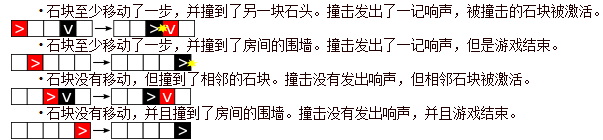
\includegraphics{temple.png}

给定$n,x$,要你构造一组解。
\subsubsection{数据范围}
保证$n$是偶数,令$n=2k$

$n \le 300,x \le k^3-k^2$
\subsubsection{题解}
构造题……也不知道怎么写题解。

对于$n=100,x=10^5$,官方题解给出了这么一个图形:

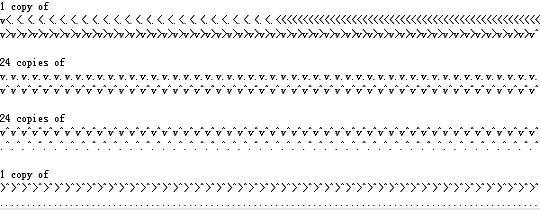
\includegraphics{temple_solution.png}

大概就是说这么一个图形是符合题目要求的。
\subsubsection{时空复杂度}
时间复杂度:$O(n^2)$

空间复杂度:$O(n^2)$
\subsection{Codeforces 317E Princess and Her Shadow}
\subsubsection{题意}
给你一个平面直角坐标系,有一个公主和一个影子,还有$n$棵树,公主在$(vx,vy)$,影子在$(sx,sy)$,第$i$棵树在点$(x_i,y_i)$。

公主要去追影子。

公主向右走,影子就会向右走;公主向左走,影子就会向左走;公主向上走,影子就会向上走;公主向下走,影子就会向下走。

不过,如果影子的那个方向是一棵树,影子就不会动。公主不能撞树。

求一组公主的行动方案,让公主抓到影子,要求行动方案长度不能超过$10^6$。如果无解输出-1。
\subsubsection{数据范围}
$n \le 300$

$|x|,|y| \le 100$
\subsubsection{题解}
一个比较厉害的构造题。

找一条公主向影子的最短路,走。

如此循环很多次。

如果足够多次之后,他们坐标仍然在$[-100,100]$的范围内并且公主抓不到影子,就可以看做无解了,因为正常情况下,会出现他们在的某一维坐标在$[-100,100]$范围以外的情况。

只要这样的话,公主的活动就自由了,她就能想办法找一棵树,让影子往那棵树上撞,然后公主就能沿着方向一直走直到横坐标相同。

接下来,公主能再找一棵树,让她们纵坐标相同。

这样就抓到影子了。
\subsubsection{时空复杂度}
时间复杂度:疑似$O(n^3)$

空间复杂度:$O(n+200^2)$
\subsection{Codeforces 269D Maximum Waterfall}
\subsubsection{题意}
要在一个墙上做人造瀑布。

有$n$个平行于$x$轴的木板,第$i$个木板有三个参数$l_i,r_i,h_i$,表示一条左端点是$(l_i,h_i)$右端点是$(r_i,h_i)$的线段。

墙高为$t$,我们不妨把墙的顶端也看做是一个$(-10^9,t)$到$(10^9,t)$的木板。

不妨再把墙的底端看作是一个$(-10^9,0)$到$(10^9,0)$的木板。

为了让瀑布漂亮,水可以从木板$i$流向木板$j$当且仅当:

\begin{enumerate}
\item $max(l_i,l_j)<min(r_i,r_j)$,可以称作$i,j$在水平方向上相交。
\item $h_j<h_i$,可以看做是$j$在$i$下方。
\item 不存在$k,h_j<h_k<h_i$,满足$i,k$与$j,k$均在水平方向上相交。
\end{enumerate}

木板$i$向木板$j$能流的流量是$min(r_i,r_j)-max(l_i,l_j)$。

一个瀑布可以看做是一个木板序列,以墙顶端木板为开头,墙底端木板为结尾,对于除了底端木板以外的任意木板,都能向他的下一个木板流水。

一个瀑布的流水量看作是每相邻两块木板的流水量的最小值。

最大化瀑布流水量。
\subsubsection{数据范围}
$n \le 10^5$

保证没有两条线段在平面上相交。
\subsubsection{题解}
一个很重要的性质是:$i$能流到$j$的点对$(i,j)$是$O(n)$的。

证明就是说,能流到$j$的木板,要么是完全被$j$包含,要么是与$j$相交。然而与$j$相交的最多只有$2$个,而如果一个木板完全被$j$包含,它就只能流到$j$了。综上所述,点对是$O(n)$的。

也就是说,对于木板$j$,设$dp[i]$表示以木板$i$为结尾的瀑布流量最大值,我们依次遍历所有的能流到$j$木板,更新$dp[i]$即可。

关键是要怎么依次遍历。

我们将木板按$h$排序,从高向低扫过去,加入一条$(l_i,r_i,h_i)$的线段,可以理解为给区间$[l_i,r_i]$赋值为$h_i$的颜色。

更新答案就是枚举所有与当前线段相交的颜色段,统计的过程中删除被他包含的所有颜色段,然后给区间染色,这样子不能保证每次枚举到的都能流到这个线段,但根据一模一样的证明方法,我们仍然能证明有小的枚举次数是$O(n)$的。

这个数据结构一般都是用线段树写的,但事实上set也能实现这个操作,还能简化代码。
\subsubsection{时空复杂度}
时间复杂度:$O(n \log n)$

空间复杂度:$O(n)$
\subsection{USACO Open Contest 2009,Tower of Hay*}
\subsubsection{题意}
给你$n$个干草堆,每个干草堆宽为$w_i$,高为$1$。

你要把它们分成若干段,搭起来。假设分成了$k$段,你就按顺序把它们打成$k$层,假设第$i$段是$[l,r]$,第$i$层的宽度就等于$\sum\limits_{i=l}^r w_i$。

要求$w_1 \le w_2 \le w_3 \ldots \le w_k$。求$k$的最大值。
\subsubsection{数据范围}
$n \le 10^5$
\subsubsection{题解}
这题做法很巧妙。

先要了解一个结论,在多种可行的堆叠方案中,至少有一种能使层数最高的方案同时使得底边最短。即底边最短的,层数一定最高。

证明如下。

任意取出一个能使层数最高在此前提下底边最短的方案,设有$n_1$层,把其中从下往上每一层最大的块编号记为$A_i$;任取一个能使底边最短在此前提下层数最高的方案,设有$n_2$层,把其中从下往上每一层最大的块编号记为$B_i$。

反证法,则要求$A_1 > B_1,A_{n_2} < B_{n_2}$,这说明至少存在一个$1<k<n_2$,满足$A_{k-1} \ge B_{k-1}$且$A_k \ge B_k$。也就是说,方案一第$k$层完全被方案二第$k$层包含。构造一个新方案,第$k$层往上按方案一,往下按方案二,两边都不要的块放中间当第$k$层。新方案的层数与方案一相同,而底边长度与方案二相同。矛盾。

这样子的转化了之后,我们就可以设$dp_i$表示$i \sim n$的干草堆所能得到的塔的底层最短是多少,同时可以利用$dp$的决策值求出$g$。

$dp$的转移方程为$dp_i=\min(sum_j-sum_{i-1})$,要求$sum_j-sum_{i-1} \le g_{j+1}$。$sum$是前缀和数组。

当然这样子是$O(n^2)$的,注意到单调性后,能用单调队列优化至$O(n)$。
\subsubsection{时空复杂度}
时间复杂度:$O(n)$

空间复杂度:$O(n)$
\subsection{Google Code Jam 2011 World Finals C Program within a Program*}
\subsubsection{题意}
无限长的道路上有一个机器人要去投递一份蛋糕,道路上每隔一英里就有一根电线杆。你需要控制机器人向东移动恰好$n$英里并放下蛋糕。

你要设计一些规则,使得机器人照着规则执行后能够正确地投递蛋糕。

这些规则必须以下述的形式呈现:<$S$> <$M$> -> < 操作>

这表明了当下列所有的条件都满足时:

\begin{enumerate}
\item 现在机器人正处于状态$S$。
\item 机器人现在所处电线杆上的标记为$M$。
\end{enumerate}

那么机器人将会执行下列的操作之一:
\begin{enumerate}
\item 若<操作>的形式为<$D$><$NS$> <$NM$>,其中$D$表示下一步移动的方向(东还是西),$NS$表示机器人的新状态,$NM$表示当前电线杆的新标记,则机器人将修改当前所处电线杆上的标记,改变自身状态,然后继续移动。
\item 若<操作>的形式为$R$(单个字母),则机器人将会在当前位置放下蛋糕,并结束任务。
\end{enumerate}

要求不能有两个规则的$S$与$M$相同,任意时刻机器人会在规则中找到一个$S$为当前机器人状态$M$为当前电线杆状态的规则,找不到就失败了。

在所有的规则中,机器人的所有状态以及电线杆上的所有标记都必须保证绝对值不超过$10^6$。现在假定机器人初始位置为原点,初始状态为$0$,并且所有电线杆上的标记初始时都是$0$。

$n$给定。你为机器人编写的程序最多只能包含$30$条规则,而且必须保证机器人能在$1.5 \times 10^5$步之内结束任务。
\subsubsection{数据范围}
$n \le 5000$
\subsubsection{题解}
神一般的构造题。

题解给出这么一个构造思路:

刚开始把$n$的二进制形式按位一次标记在电线杆上,通过一些操作,使得每一步都能让电线杆对应的二进制数减$1$,并向后移动一位。

这个思路真的很神啊!

用程序可以做到实现这个操作,缩缩行之后我恰好$30$步。

那么就在这里举一个$n=5000$的例子好了:

30

0 0 -> E 1 100

1 0 -> E 2 100

2 0 -> E 3 100

3 0 -> E 4 101

4 0 -> E 5 100

5 0 -> E 6 100

6 0 -> E 7 100

7 0 -> E 8 101

8 0 -> E 9 101

9 0 -> E 10 101

10 0 -> E 11 100

11 0 -> E 12 100

12 0 -> E 13 101

13 0 -> W 200 0

200 100 -> W 200 100

200 101 -> W 200 101

200 0 -> E 201 0

201 100 -> E 202 0

201 101 -> E 203 0

202 100 -> E 202 101

202 101 -> E 203 101

203 100 -> E 203 100

203 101 -> E 204 100

204 100 -> E 203 101

204 101 -> E 204 101

203 0 -> W 205 0

205 0 -> E 207 0

207 0 -> R

205 101 -> W 200 101

204 0 -> W 200 101

\subsubsection{时空复杂度}
时间复杂度:$O(\log n)$

空间复杂度:$O(1)$
\subsection{Google Code Jam World Final 2013 E Let Me Tell You a Story}
\subsubsection{题意}
给你一个长度为$n$的序列$a_1,a_2,\ldots,a_n$。

要你每次删除一个数。如果某个时刻数组$a$变成了一个单调不递增序列,就停止。

求删除的操作序列方案数。
\subsubsection{数据范围}
$n \le 2000$
\subsubsection{题解}
原题题意非常冗杂,但是看懂了题意之后的确是这么一个意思。

我们可以用树状数组在$O(n^2 \log n)$的时间里预处理出$sum[i][j]$为以第$i$个数结尾的长度为$j$的单调不递增序列的方案数。

也就是我们能预处理出$dp_i$表示长度为$i$的单调不递增序列的方案数。

对于一个长度为$i$的单调不递增序列,我们有$(n-i)!$的方案得到他。

但问题在于,会有不合法方案,所谓不合法方案,指的是某一个时刻里,序列变成了一个单调不递增序列。如何去除这种情况是关键。

如果我把一个序列删成了单调不递增序列,那么再怎么删,他仍然是单调不递增序列。换句话说,如果有这种情况,就一定会在删成长度为$i+1$的序列的时候,得到的序列是单调不递增序列。

删成这个有$(n-i-1)!$的方案数,接下来要删成长度为$i$的序列又有$i+1$的方案数。

所以答案为$\sum\limits_{i=1}^n (n-i)!dp_i-(n-i-1)!(i+1)dp_{i+1}$。

$sum$能用滚动数组优化,空间可以做到$O(n)$。
\subsubsection{时空复杂度}
时间复杂度:$O(n^2 \log n)$

空间复杂度:$O(n)$
\subsection{Codeforces 264E Roadside Trees}
\subsubsection{题意}
现在有$1 \sim n$这些位置能种树。刚开始没有树。

第$i$个时刻,可能会发生如下的一件事件:

\begin{enumerate}
\item 在某个没有种过树的位置$p_i$,种一棵高度为$h_i$的树。
\item 砍掉第$x_i$个树,保证这个位置以后不会再种树。
\end{enumerate}

每天每棵树会长高$1$。

每执行一个操作,要求输出最长上升子序列长度。
\subsubsection{数据范围}
$n \le 10^5$

$x_i,h_i \le 10$

任意时刻每棵树的高度互不相同。
\subsubsection{题解}
每天长高一米的问题,我们能用一个变量记录整体长高多少,插入一个树时能把高度变换一下,就能处理了。

所以以下均建立在高度不变的情况下。

这相当于是一个动态LIS问题,不知道有没有什么直接做的方法……反正我是不会

但是注意到,这个题目有一个非常重要的性质:$x_i,h_i \le 10$。

有了这个性质,我们就能暴力进行更新。

大概就是说,我设$dp_i$表示以$i$为开头,能得到的最长的上升子序列长度。

在$a_0$处插入负无穷大,答案即为$dp_0$。

由于保证$x_i,h_i \le 10$,以及保证任意时刻树的高度互不相同。

所以插入一棵树的时候,要修改一个位置的$dp$值,那个位置的高度必须小于他的高度,所以最多修改$O(h_i)$个点的$dp$值,可以暴力。

砍掉第$x_i$棵树,要修改一个位置的$dp$值,那个位置的编号必须小于他的编号,所以最多修改$O(x_i)$个点的$dp$值,可以暴力。

至此,问题基本解决,还有一个无足轻重的小问题是怎么快速求一个点的$dp$值,以及判断一个点是否要修改。

我的做法是不仅求$dp$值,还对每个$i$开个set,把$dp$值等于$i$的丢入set里去。

我们能用这么一个办法在$O(\log n)$时间里判定$dp_i$能否大于等于$x+1$:在$x$对应的set里找$i$的后继,如果$i$能接在他前面就可以大于等于$x+1$,否则不行。

用这个办法,插入一个点时,我们能二分求出他的$dp$值,更新时也能判定他要不要修改。
\subsubsection{时空复杂度}
时间复杂度:$O(n \log^2 n+100n\log n)$

空间复杂度:$O(n)$
\newpage
\section{试题泛做4}
\subsection{Codeforces 293E Close Vertices}
\subsubsection{题意}
给你一棵$n$个点的树,第$i$条边长度为$1$,边权为$w_i$。

给你两个参数$L,W$,求有多少点对$(i,j)$,满足路径$i \rightarrow j$的长度不超过$L$,边权不超过$w_i$。
\subsubsection{数据范围}
$n \le 10^5$
\subsubsection{题解}
显然使用点分治算法。

因为求得是点对数,具有可减性,显然用补集转化。

我们要做的是查询$n$个点中,每个点$i$有两个参数$dep_i,dis_i$,求有多少点对$(i,j)$,满足$dep_i+dep_j \le L,dis_i+dis_j \le W$。

我们将他们按$dis$排序,根据单调性扫,每次插入删除,保证当前元素的$dis$符合要求,求$dep$在某个范围内的点数。

能用树状数组方便的实现。
\subsubsection{时空复杂度}
时间复杂度:$O(n \log^2 n)$

空间复杂度:$O(n)$
\subsection{Codeforces 306C White, Black and White Again}
\subsubsection{题意}
接下来$n$天,会有$w$件两两不同的好事以及$b$件两两不同的坏事,每天至少发生一件事情,每天要么全部发生好事要么全部发生坏事。

$n$天,会先是若干天发生好事,再是若干天发生坏事,再是若干天发生好事。

求方案数(每天发生的事情的顺序不同也算不同)。
\subsubsection{数据范围}
$n \le 4000$

$w,b \le 4000$
\subsubsection{题解}
联赛难度题。

先枚举$i,j$,表示$[1,i)$天发生好事,$[i,j]$发生坏事,$(j,n]$发生好事。

只要能$O(1)$计算就行了。

首先,我们可以假设事情发生顺序没有影响。(因为这样算出来的答案乘上$w!b!$就是正确答案了。)

那么要做的就是将$b$个数分成$j-i+1$段,$w$个数分成$n-(j-i+1)$段。

将$n$个数分成$m$段的方案数相当于在$n-1$个空里插入$m-1$个空,应该是${{n-1} \choose {m-1}}$

预处理阶乘及其逆元,可以$O(1)$计算组合数。

这样就没了。另外显然我们不需要枚举$i,j$,只需要枚举$j-i$,这样复杂度就是$O(n)$的,不过反正$O(n)$和$O(n^2)$都是很水的,我就没有去管了。
\subsubsection{时空复杂度}
时间复杂度:$O(n^2)$

空间复杂度:$O(n)$
\subsection{Codeforces 331E2 Deja Vu*}
\subsubsection{题意}
有$n$个点,$m$条有向边,每条边上有个序列。

无重边,无自环。

称一条路径的“点序列”为经过的点所构成的序列,“边序列”为每条边上的序列拼起来。

如果一条路径的“点序列”与“边序列”完全一致,称其为“WOW”序列。

求有多少长度为$1,2,\ldots,2n$的“WOW”序列。
\subsubsection{数据范围}
$n \le 50$

边上序列长度总和$\le 10^5$
\subsubsection{题解}
称极小“WOW”路径为没有子路径是“WOW”的路径。

关键思想是找出极小“WOW”路径,用$dp$将他们拼起来。

先来看怎么找极小“WOW”路径。

一个显然的想法是,如果我枚举从$i$出发的一条边,这条边不是空边,那么他就会一直顺着边上的序列走下去,一直某个点恰好点序列与边序列匹配为止。

但是很麻烦的情况却是有可能会是空边。如果是空边的话,就不知所措了。

但是我们不妨换一个思路来看待问题。这样子的路径,一定能找到边$(u,v)$,使得$(u,v)$边上的序列存在相邻的$(u,v)$,然后从$u$开始向前顺着边上序列走下去,$v$开始向后顺着边上序列走下去,就能得到了。

因为点序列每次都是恰好加$1$,所以极小“WOW”路径一定恰好存在一条边,能让我这样找到。

这么做的复杂度应该是不超过$O(n^3)$的。我们能找出所有的极小“WOW”路径。

是不是说,找出极小“WOW”路径,用空边拼起来,就能得到所有“WOW”路径了呢?其实不然。

考虑有个“WOW”路径,他的终点连向点$1$,边上的序列是$1$,这也是一条“WOW”路径,但它并不是由两条“WOW”路径用空边拼起来的。

所以我们还要找到极小类“WOW”路径,就是说计算有多少路径,使得点序列去掉开头那个点或者去掉结尾那个点能与边序列匹配。还要求路径极小。

用找极小“WOW”路径的方法能够找出来。

我们可以用dp将极小“WOW”路径和极小类“WOW”路径拼起来,称为次小“WOW”路径。这一步的复杂度应该是$O(n^4)$的。

然后就是每次把一个“WOW”路径和一个次小“WOW”路径拼起来。直接搞应该是$O(n^5)$的,注意到我们要求的并不是从$i$到$j$经过$k$条边的方案数,而是从$i$出发经过$k$条边的方案数。

改改状态的定义,就可以降为$O(n^4)$了。
\subsubsection{时空复杂度}
时间复杂度:$O(n^4)$

空间复杂度:$O(n^3)$
\subsection{Google Code Jam 2009 Final A Year of More Code Jam}
\subsubsection{题意}
$n$天里会举行$T$场大赛。

第$i$场大赛会有$m_i$场小比赛,有一个比赛上线时间,第$j$场小比赛的比赛时间是上线时间的$d_{i,j}$天后。

比赛上线时间均匀的分布在$n$天里,也就是总共有$n^T$种方式。

定义愉悦值为$\sum\limits_{i=1}^n s_i^2$,$s_i$表示有几场比赛在今天举行。

求期望愉悦值。要求你用一个$K+\frac{A}{B}$的分数形式输出!
\subsubsection{数据范围}
$n \le 10^9$

$m_i,T \le 50$
\subsubsection{题解}
虽然直接做是很好做的,但是往往避免不了写高精度的命运,一旦这样的话时间复杂度就无法通过了。

平方往往能够转化为点对个数。

转化之后,若第$a$场比赛的第$b$场小比赛与第$c$场比赛的第$d$场小比赛在同一天,会给愉悦值带来$1$的贡献。

这么一来的话,我们来看他会给期望带来多少的贡献。

让$a$场比赛的第$b$场小比赛与第$c$场比赛的第$d$场小比赛在同一天,记作事件$(a,b,c,d)$,$a,c$的上线时间方案数是很好算的,假设有$S$种方案。

来看另外的$T-2$场比赛,无论他们什么时候上线,事件$(a,b,c,d)$仍然成立。

所以事件$(a,b,c,d)$对期望的贡献应该是$\frac{Sn^{T-2}}{n^T}=\frac{S}{n^2}$。

这样的话,就可以避免写高精度了。
\subsubsection{时空复杂度}
时间复杂度:$O(T^2m^2)$

空间复杂度:$O(Tm)$
\subsection{Codeforces 321D Ciel and Flipboard*}
\subsubsection{题意}
有一个$n$行$n$列的板子,每个格子上有一个数字,$n$是奇数。

令$m=\frac{n+1}{2}$,每次可以选择一个$m$行$m$列的子矩阵,将里面的元素乘以-1。他能无限次操作。

要求最大化板子的数字和。
\subsubsection{数据范围}
$n \le 33$
\subsubsection{题解}
把操作一个矩形看做操作某个点。

很多题设的都是某个点是否操作,这样子设无法对问题带来帮助。

换个角度思考,我们设某个点有没有变号。

有这么两个等式:

$x_{i,j} \oplus x_{m,j} \oplus x_{i+m,j}=0,x_{i,j} \oplus x_{i,m} \oplus x_{i,j+m}=0$

正确性显然。对于任何一个式子,我操作一个矩形,等式左边都会修改$0$或$2$个值,得证。

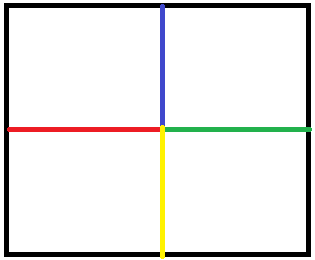
\includegraphics{ceil.png}

先来考虑一个$O(2^nm^2)$的做法。

爆枚红线、蓝线上的点。这个的复杂度是$O(2^n)$的。

爆枚了红线,蓝线之后,黄线、绿线也是已知的。

我们再来枚举左上角的每个点$(i,j)$。只要知道了点$x_{i,j}$的,我们就知道$x_{i+m,j},x_{i,j+m}$,从而知道了$x_{i+m,j+m}$。

这样的话,我们发现每个点的贡献是独立的,我们只要把$x_{i,j}=0$与$x_{i,j}=1$时,$x_{i,j}+x_{i+m,j}+x_{i,j+m}+x_{i+m,j+m}$中的较大值加入答案就行了。

这个做法,利用贡献独立的方式,巧妙地降低了复杂度。虽然仍然无法通过,但我们可以继续顺着这个思路想下去。

我们看看还有没有什么贡献是独立的。

事实上是有的,那就是红线已知了之后,蓝线的点,贡献都是独立的!

也就是说,我们爆枚红线上的点,枚举蓝线上的第$i$个点,一旦蓝线上的第$i$个点已知,左上角的$i$行的那些点的贡献就都能用上面那个方法算了。

这样的话,我们就并不需要爆枚蓝线,只要对蓝线上的每个点算贡献就行了。

最后还有一个问题:爆枚了之后如何保证有解?

首先,我们真正用到了“枚举”的,只有左上角的$m^2$个点,其余点是推出来的。换句话说,只要左上角$m^2$个点有解,就能有解了。

现在有这么一个问题:你每次能把一个大小为$m$行$m$列的子矩形反色,要求左上角的$m$行$m$列的每个点都是某种颜色,其他点的颜色随意。有没有无解的情况。

这是一个很经典的贪心构造问题,每次贪心的让一个点颜色变对,是一定能构造出解的,于是这么做就没问题了。
\subsubsection{时空复杂度}
时间复杂度:$O(2^m m^2)$

空间复杂度:$O(n^2)$
\subsection{USACO December Contest 2010,Threatening Letter}
\subsubsection{题意}
给你两个串$A$,$B$。

你要把串$A$分成若干段,每一段都是串$B$的子串。

求最少能分成多少段。
\subsubsection{数据范围}
$|A|,|B| \le 50000$
\subsubsection{题解}
首先这个问题是能贪心的,即每次砍去$A$最长的一段前缀,要求这个前缀是$B$的子串。

预处理出后缀数组,我们判断一个串是不是$B$的子串,只要计算他与某个后缀的LCP就行了,这个是$O(1)$的。

所以暴力贪心,利用后缀数组暴力判断就行了。

你也可以写个后缀自动机在上面暴力跑。
\subsubsection{时空复杂度}
时间复杂度:$O(n \log n)$

空间复杂度:$O(n)$
\subsection{Google Code Jam 2009 Final C Doubly-sorted Grid}
\subsubsection{题意}
一个$R$行$C$列的长方形网格,每一格有一个字母。要求按照字典序,从左往右单调递增,从上往下单调递增。

比如下面的例子中,前两个合法,后两个不合法。

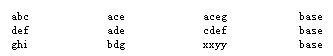
\includegraphics{doubly-sorted.png}

现在给你这个网格,有些位置已经填了字母,有些位置没有填,求合法网格方案数。
\subsubsection{数据范围}
$R,C \le 10$
\subsubsection{题解}
我们考虑按字母顺序一个一个填。

假设我填了前$i$个字母,那么在图形中前$i$个字母一定会构成一个右边界单调不递增的图案。

我们可以用这个图案来描述状态,状态数应该是${20 \choose 10}$的,只有$184756$个。

设$dp[i][S]$为填了$i$个字母,状态是$S$。暴力的转移方法应该是枚举下一个字母的右边界图形。这样子的复杂度比较高,由于是求和,我们考虑用前缀和优化。

那么就应该是$dp[i][S]=\sum dp[i-1][S']$,满足$S'$的任何一位都小于$S$的任何一位,$S'$是一个合法图形,并且如果输入中给出了$i-1$这个字母的一些位置,$S'$还要满足输入。

用前缀和不好$O(1)$直接算出来。我们不妨一位一位的来看,像数位$dp$一样,枚举最后一个小于$S$的位置,开$R$个前缀和数组。这样就行了。
\subsubsection{时空复杂度}
时间复杂度:$O(26R{2C \choose C})$

空间复杂度:$O(R{2C \choose c})$
\subsection{USACO Open Contest 2007, Connect}
\subsubsection{题意}
有一个$2 \times m$的网络。

有$m$个操作,操作可能是插入一条边,删除一条边(插入,删除的边都是网络上相邻的,即假设插入或删除一条点$(a,b)$到点$(c,d)$的边,有$|a-c|+|b-d|=1$)。

同时操作也可能是询问点$(a,b)$能否走到点$(c,d)$。注意一个限制条件是他们必须得在以$(1,\min(b,d))$为左下角,$(2,\max(b,d))$为右上角的矩形里走,就是说他们所在的列必须一直在$b$与$d$之间。

强制在线。
\subsubsection{数据范围}
$m \le 15000$
\subsubsection{题解}
这是上海一道省选题的弱化版。

做法是线段树。

我们用线段树维护一个矩形的四个角相互之间的连通性。也就是维护${4 \choose 2}=6$个域。

合并区间时,可以用两个区间共$12$个域的信息,以及连接两个区间的那两条边是否存在,得到大区间的信息。
\subsubsection{时空复杂度}
时间复杂度:$O(n \log n)$

空间复杂度:$O(n)$
\subsection{Codeforces 261E Maxim and Calculator}
\subsubsection{题意}
你刚开始有一个二元组$(1,0)$。

设当前二元组为$(a,b)$,每次能变成$(a,b+1)$或者变成$(ab,b)$。

在区间$[l,r]$内,有多少$x$,可以操作不超过$p$步,让你的二元组的第一维变成$x$。
\subsubsection{数据范围}
$2 \le l \le r \le 10^9$

$1 \le p \le 100$
\subsubsection{题解}
算是一个爆搜题吧。

首先,能用$100$以内的质数表示出来的数字,只有不到$3 \times 10^6$。可以全部找出来。

设把$(a,b)$变成$(a,b+1)$为操作一,把$(a,b)$变成$(ab,b)$为操作二。

先枚举最终的$b$。也就是强行认为要做$b$次操作$1$。

求$dp[i]$表示在做不超过$b$次操作一的情况下,凑出$i$最小要几次操作二。

枚举所有能被$b$整除的$i$,用$dp[i/b]+1$去更新$dp[i]$。

若满足$dp[i]+b \le p$,则认为$i$能够得到。

由于光是循环就要进行近三亿次,所以需要加点常数优化。
\subsubsection{时空复杂度}
时间复杂度:$O(3000000p)$

空间复杂度:$O(3000000)$
\subsection{Google Code Jam World Final 2009 E Marbles*}
\subsubsection{题意}
有$2n$个珠子在$x$轴上,珠子有$n$种颜色,每种颜色有$2$个。珠子的横坐标是$1,2,\ldots,2n$。

要求你用$n$根线,把同色珠子都连起来,任意两根线线不能允许相交。

每根线得是形如$(x_1,0) \rightarrow (x_1,y) \rightarrow (x_2,y) \rightarrow(x_2,0)$的形式,要求$y$是整数(允许是负数,不能是$0$),$x_1,x_2$上的珠子颜色相同。

称这样的线的高度是$y$。

给你第$i$个珠子的颜色,要求最小化最高的线与最低的线的高度差。

$T$组数据。
\subsubsection{数据范围}
$n \le 500$

$T \le 50$
\subsubsection{题解}
首先来看约束条件。

每根线可以看做一个区间,如果两个区间相交却没有包含关系,他们就不能同时在上面也不能同时在下面。

这是一个二分图关系。

换句话说,我们把在上面的看做白点,在下面的看做黑点,相交而不包含的区间连边,一组合法方案就是一个二分图。

对于一个联通二分图,只要第一个点的颜色确定,整个二分图的颜色都确定了。

我们对于一个联通二分图,记录第一个点是白色时,最大值与最小值。

问题转化为,有若干个联通二分图,要你给每个二分图的第一个点确定颜色,然后得到的图的最大值减最小值最小。似乎还是很难做。

观察后可以得到这么几个性质:

对于任意区间$A,B$,若$A,B$不在同一个二分图里,他们要么包含要么相离。

此外对于联通二分图$A$和$B$,若$A$的区间$a$被$B$的某个区间$b$包含,区间$b$就会包含整个$A$。

有了这个性质,二分图$A$和$B$要么是相离关系,要么可以看做完全包含关系。

我们对于每个二分图,找到包含它的最小二分图,这样子会构成一个树关系。

另外加入一个根指向所有没有被包含的二分图。

预处理一些东西之后,就可以做树形$dp$了。$dp$部分有点复杂。
\subsubsection{时空复杂度}
时间复杂度:$O(n^2T)$

空间复杂度:$O(n^2)$
\subsection{Codeforces 264D Colorful Stones}
\subsubsection{题意}
有两个串$s$与$t$。

字符集只有RGB三种。

刚开始有两个人分别在两个串的开头,记作$(1,1)$。

假设你当前在$(x,y)$,若$s_x=s_y$,下一步能转移到$(x+1,y+1)$,否则能转移到$(x,y+1)$或者$(x+1,y)$。

但是任意时刻不允许任何一个人走到串外面。
\subsubsection{数据范围}
$|s|,|t| \le 10^6$
\subsubsection{题解}
记$l_i$表示第一个人在\textbf{前}$i$个位置时第二个人能走到的最小值,$r_i$表示第一个人在\textbf{前}$i$个位置时第二个人能走到的最大值。

一个错误的做法是认为答案是$\sum\limits_{i=1}^n r_i-l_i+1$。

但这样是有反例的,比如串$s$是$RG$,串$t$是$GR$,那么$l_2=1,r_2=2$,可是却无法转移到$(2,2)$。

题解表示说,这个反例虽然存在,神奇的却是他是唯一的反例。也就是说,假设当前在$i$,我只要减去$[l_i+1,r_i]$里有多少个$j$,使得$t_j=s_{i-1},t_{j-1}=s_i$就行了,由于字符集只有$3$,可以预处理前缀和数组。
\subsubsection{时空复杂度}
时间复杂度:$O(9n)$

空间复杂度:$O(9n)$
\subsection{Google Code Jam World Final 2010 C Candy Store*}
\subsubsection{题意}
要你预先选一个可重数集。

有$n$个人,每个人会选择$[1,C]$的一个正整数。

然后无论对方怎么选,你都要能在预选的可重数集里取出若干个不相交的子集,第$i$个子集内的数字和等于第$i$个人的数。

要你构造数集大小最小的方案。

$T$组数据。
\subsubsection{数据范围}
$1 \le T \le 100$

$1 \le k \le 1000,1 \le C \le 10^{12}$
\subsubsection{题解}
设$a_1 \le a_2 \le a_3 \cdots \le a_m$,若存在$i$使得$n(a_i-1)> \sum\limits_{j=1}^{i-1} a_j$,那么所有客人都购买$a_i-1$就实现不了了,所以我们得到了一个下界。

那么如何证明他的合法性呢?我们都知道有一种错误的贪心方法,是每次找到一个最大的比他小的,依次做下去。

但是反过来,如果我们把题意的选出若干个子集改成按这个方法来贪心,发现这个解符合要求,那么对于本题,解当然也符合要求。

用数学归纳法是可以证明的。即证明这种方法构造出来的对于$n$可行,当$n=1$时显然,然后$n>1$时,无论对手选了一个什么数,贪心法干掉他之后仍然满足对于任意的$i$都使得$n(a_i-1) \le \sum\limits_{j=1}^{i-1} a_j$。
\subsubsection{时空复杂度}
时间复杂度:$O(n \log C)$

空间复杂度:$O(1)$

\subsection{Codeforces 342D Xenia and Dominoes}
\subsubsection{题意}
一张$3$行$n$列的网格,要在上面放多米诺骨牌。

有一些位置是禁止点表示不能放,有恰好一个圆圈,你也不能放多米诺骨牌。

要求用$1 \times 2$和$2 \times 1$的多米诺骨牌放满除圆圈和禁止点以外的所有点,并要求,有一个横向的多米诺骨牌正对着圆圈。

求方案数。
\subsubsection{数据范围}
$n \le 10^4$
\subsubsection{题解}
简单的状压$dp$即可。

状态记当前轮廓线上的$m$个点的信息,转移。

为了处理圆圈,我们再额外记录一下圆圈问题是否已经被解决。
\subsubsection{时空复杂度}
时间复杂度:$O(2^3 n)$

空间复杂度:$O(2^3)$
\subsection{Codeforces 273E Dima and Game}
\subsubsection{题意}
两个人在玩博弈游戏。

纸上有$n$对数$l_i,r_i(1 \le l_i < r_i \le p)$,玩家轮流操作,操作过程如下:

\begin{enumerate}
\item 选择某一对数,假设选择了第$i$对,要求满足$r_i-l_i>2$。
\item 将这对数换成$(l_i+\lfloor \frac{r_i-l_i}{3} \rfloor,l_i+2\lfloor \frac{r_i-l_i}{3} \rfloor)$,或者换成$(l_i,r_i-\lfloor \frac{r_i-l_i}{3} \rfloor)$。
\end{enumerate}

不能操作的人算输。给定$n,p$,求先手获胜的方案数。
\subsubsection{数据范围}
$n \le 1000$

$p \le 10^9$
\subsubsection{题解}
$SG$题。

朴素的看待这个问题,$SG$函数应该是设$SG(l,r)$

可以发现对于$(l_1,r_1),(l_2,r_2)$,若$r_1-l_1=r_2-l_2$,则有$SG(l_1,r_1)=SG(l_2,r_2)$,原因见公式。

这样的话,就只要设$SG(n)$表示一个长度为$n$的区间的$SG$值了,但这也不是很好解决。

我们打表后可以发现,似乎$SG$函数值都是一段一段的,更关键的是,他的增长速度非常缓慢,可以看做是$\log$级别的速度在增长。

有了这个猜想,我们不如从$1$开始,每次二分地来暴力找出一段极长区间使得$SG$值都相同,最后会只有$O(\log p)$个区间。

有了这些区间之后,就可以暴力$dp$了,由于区间个数很少,$n$也很小,所以这题就没了。
\subsubsection{时空复杂度}
时间复杂度:$O(n+\log^2 p)$

空间复杂度:$O(n+\log p)$
\subsection{Codeforces 335E Counting Skyscrapers*}
\subsubsection{题意}
大街上有一排大楼,大楼的数量是在$2$到$314!$里随机的。

每座楼的高度是随机的,高度为$i$的概率是$2^{-i}$。如果他有$i$层,那么他的楼层的编号是$0 \sim i-1$。

大楼间有一些滑索。一座大楼的第$i$层和另一座大楼的第$i$层之间有滑索当且仅当两楼之间没有大楼有第$i$层。

Alice想知道大楼数量的准确值。于是她把计数器初始化为$1$,从最左边的大楼开始往右走,每次走到一个大楼就把计数器加上$1$,直到她到达最右边的大楼。

Bo想尽快完成任务。于是他把计数器初始化为$1$,从最左边的大楼开始利用滑索从一座大楼滑到另一座。每次他会忽略那些高度(即所在楼层编号)大于$h$的滑索,然后在剩下的往右滑的滑索中选一个最高的,将计数器加上$2^i$,其中$i$是他当前所在的楼层编号。他会一直持续这个过程直到他到达最右边的大楼。

现在给你Alice的计数器值或者Bob的计数器值,求另一个人的计数器的期望值。

计数器值是$n$,$h$是Bob愿意使用滑索的最高楼层编号。
\subsubsection{数据范围}
$n \le 30000$

$h \le 30$
\subsubsection{题解}
完全不会的神题。

$314!$可以看做$\infty$。

考虑Bob的情况。

假设Bob走过一段高度为$h_t$的滑索,再设中间$L-1$个大楼的高度小于$h_t$。

来算这种情况的概率,应该是$\frac{(1-2^{-h_t})^{L-1}}{\sum_{k \ge 1} (1-2^{-h_t})^{k-1}}$。

这个等于$2^{-h_t}(1-2^{-h_t})^{L-1}$。

然后算期望,可以发现Alice的计数器期望增加$2^{h_t}$,也就是期望有$2^{h_t}$的连续大楼高度小于$h_t$。

而Bob的计数器变化正好是$2^{h_t}$,于是我们发现如果已知的是Bob,Alice的期望神奇的是$n$。

考虑Alice的情况。

直接做的复杂度是$O(nh^2)$的,做法是$dp$,$dp$有点复杂。

考虑这么来思考,先让$h=0$,显然Bob的期望值是$n$。

考虑让高度从$h-1$变成$h$,计算增量。由于期望可加,我们只要把增量都加起来就行了。

把$h-1$变成$h$时,相当于说原来高度为$h-1$的摩天楼中有一些变成了$h$,考虑这种事件的贡献。

假设Bob经过了一条绳索,这条绳索经过了$l$个大楼(不考虑左端点考虑右端点),这种情况的概率是$2^{-2h}(1-2^{-h})^{l-1}$。

增加量则是$2^h$。

再来考虑损失量。要求中间高度为$h-1$的摩天大楼的期望数加$1$。

列出式子来应该是$((l-1)\frac{2^{-h}}{1-2^{-h}}+1)2^{h-1}=(\frac{l-1}{2^h-1}+1)2^{h-1}$。

把它们全部加起来并化简为:\[\sum_{l=1}^{n-1} (n-l)2^{-h}(1-2^{-h})^{l-1}(\frac{1}{2}-\frac{1}{2} \times \frac{l-1}{2^h-1})\]。

我们得到了一个时间复杂度为$O(nh)$的做法。
\subsubsection{时空复杂度}
时间复杂度:$O(nh)$

空间复杂度:$O(1)$
\newpage
\section{试题泛做5}
\subsection{Codeforces 351D Jeff and Removing Periods}
\subsubsection{题意}
假如有一个长度为$n$的数列$a_1,a_2,\ldots,a_n$

你允许对它进行操作,操作如下:
\begin{enumerate}
\item 首先选择三个整数$v,t,k$,满足$a_v=a_{v+t}=a_{v+2t}=\ldots=a_{v+kt}$
\item 然后将其删除,可以得到一个新的数列。
\item 你能将新数列重排
\end{enumerate}

现有一个长度为$m$的数列,$q$个询问,每次询问$[l,r]$表示要你通过上面的操作将$[l,r]$的数删除的最小步数。
\subsubsection{数据范围}
$m,q,b_i \le 10^5$
\subsubsection{题解}
这个操作最重要的特点在于,它能够重排。也就是说,除了第一次操作,后面的操作是我们来定的。

先考虑问题下界,显然为区间内不同数的个数;紧接着考虑上界,我们容易发现,操作完第一次后,我们可以每次把相同的数放在一起,从而能一次消干净一类数。

于是上界是区间内不同数的个数+1,问题在于何时能得到下界。

经思考后容易发现,能否得到下界,在于我们第一步能不能消干净一类数。于是此题化为两个子问题:

\begin{enumerate}
\item 求区间内不同数的个数
\item 求区间内是否存在一列数,他们的位置是等差数列
\end{enumerate}

对于第一问是经典问题,可以用树状数组离线$O(n \log n)$做,也可以用主席树在线$O(n \log n)$做

对于第二问,预处理$R_i$表示以$i$为起点向右等差数列形式最多延伸到哪里,$last_i$表示上一个和$i$相等的数。

问题转化为了我们要在$[l,r]$里找到$last_i<l$的$R_i$的最大值,主席树维护即可。因为这一步用了主席树,所以给主席树加个域就能顺便把第一问做了。

\subsubsection{时空复杂度}
时间复杂度:$O(n \log n)$

空间复杂度:$O(n \log n)$
\subsection{Codeforces 241B Friends}
\subsubsection{题意}
现有整数$n,m$,以及一个长度为$n$的数组$a$。求数组里所有数对的异或值的前$m$大的和。
\subsubsection{数据范围}
$n \le 50000$
\subsubsection{题解}
首先给定一个数列,询问与某个数的异或值的最大值是个能用trie树解决的经典问题,在此不再赘述。

这题的做法比较显然,我们可以二分第$m$大的值,判定方法则是利用trie树,对每个点维护子树内有多少个点。

接下来要做的,就是查询异或和大于某数的这些异或和的和,类似的,在tire树上对每个节点维护$sum[i]$表示子树内第$i$位为$1$的数目,如此在trie树上跑一遍,用按位处理的思想就可以利用sum数组来算贡献。以上是一种能在CF上过掉的做法,时间复杂度$O(n \log^2 n)$。

由于这题在清澄上缩短了时限,所以需要卡一点常数。我们发现二分第$m$大的值再判定的方法没有用到trie树的信息,事实上我们可以在trie树上二分,方法为先试着向左走,算右子树的总和,决定是否可以向左走(同平衡树求第k大)。如此一来,虽然后面那部分的$O(n \log^2 n)$没有优化下来,但前面已经降为了$O(n \log n)$,降低了常数

接下来再加上读入优化、取模优化等技巧,就可以通过此题
\subsubsection{时空复杂度}
时间复杂度:$O(n \log^2 n)$

空间复杂度:$O(n \log^2 n)$
\subsection{Codeforces 323B Tournament-graph}
\subsubsection{题意}
你需要构造一张$n$个点的竞赛图,使得对于任意两个点$(u,v)$,满足$u$到$v$的最短距离不大于$2$
\subsubsection{数据范围}
$n \le 1000$
\subsubsection{题解}
样例给出了$n=3$的情况,并告诉了我们$n=4$为无解

通过暴搜或者手算,我们可以知道$n=6$有解

用增量的方法进行构造

假设对于$n$个点有解,我们试图增加两个点$u,v$,可以让$u$连向这$n$个点,这$n$个点都连向$v$,再让$v$连向$u$,容易证明此构造方案合法。
\subsubsection{时空复杂度}
时间复杂度:$O(n^2)$

空间复杂度:$O(n^2)$
\subsection{USACO March Contest 2008, Land Acquisition}
\subsubsection{题意}
有$n$块土地,第$i$块土地是长宽分别为$l_i,w_i$的矩形。

你每次可以购买几块土地,花费是购买土地集合中长度的最大值$\times$宽度的最大值

要购买完所有土地,求最优方案
\subsubsection{数据范围}
$n \le 50000$
\subsubsection{题解}
这题需要发现一些性质。

对于两个土地$i,j$,若$l_i \le l_j,w_i \le w_j$,则是否存在第$i$块对答案并无影响,因为我们完全可以把第$i$个土地和第$j$个土地一起购买。因此,我们能将第$i$个土地删去。

这时,神奇的事情出现了,我们所剩下的徒弟,按$l$排序后,一定是$w$单调递减的序列!

这样的话,如果我们选了两个土地$i,j(i<j)$,自然与将$[i,j]$区间内的都选了代价是相同的,我们发现最优解一定是每次选一段区间!

如此一来,一个$O(n^2)$的dp就很显然了。

$dp[i]$表示选完$1 \sim i$的土地的最优花费。

$dp[i]=\min\{dp[j-1]+l[j]*w[i]\}$

注意到$w$是单调递增的,我们可以用斜率优化来做,时间复杂度降为$O(n)$。

如果排序是使用的基数排序,整个题都是$O(n)$的(虽然我是用快排做的)。
\subsubsection{时空复杂度}
时间复杂度:$O(n)$(如果使用基数排序)

空间复杂度:$O(n)$
\subsection{Codeforces 305E Playing with String}
\subsubsection{题意}
两人进行博弈游戏,刚开始有一张纸,纸上有一个长度为$n$的字符串。

记$[l,r]$表示一个字符串左端点为$l$右端点为$r$的子串。

一次游戏操作如流程下:

\begin{enumerate}
\item 选择一张纸进行操作。
\item 选择一个$i$,使得存在正整数$k < i$满足子串$[i-k,i+k]$为回文串。
\item 接下来将纸撕开,即一张纸分成三张纸,对应的子串是$[1,i-1]$,$[i,i]$,$[i+1,n]$。
\end{enumerate}

不能操作者负,问先手是否有必胜策略。
\subsubsection{数据范围}
$n \le 2000$
\subsubsection{题解}
SG函数的应用。

一个位置$i$能否操作是需要判断是否有$s_{i-1}=s_{i+1}$即可。

注意到如果一个位置$i$不能操作了,那么我们把原游戏看做是$[1,i-1]$与$[i+1,n]$两个子游戏的和也是可以的。

这么一来,我们把串分割成若干段,每一段的每个元素都能进行操作。这些游戏的SG和就是原游戏的SG和了。

我们计算一个长度为$i$的任意一个位置都能操作的游戏的SG值,这个是可以$O(n^2)$的预处理的。

接下来枚举第一步,然后$O(n)$判断就好了。
\subsubsection{时空复杂度}
时间复杂度:$O(n^2)$

空间复杂度:$O(n)$
\subsection{Codeforces 319D Have You Ever Heard About the Word?}
\subsubsection{题意}
若长度为$n$的字符串$S$能表示成字符串$A$循环若干次的形式,称$A$是$S$的重复块。

现有一个字符串,每次你要找到他的一个子串中的最短重复块;若有多于一个就选择最左边的。不断执行这个操作直到没有重复块为止,你要输出最后的字符串。

如$aaaabaaab \rightarrow aaabaaab \rightarrow aabaaab  \rightarrow abaaab \rightarrow abaab  \rightarrow abab \rightarrow ab$
\subsubsection{数据范围}
$n \le 50000$
\subsubsection{题解}
一个串如果是某个子串的重复块,那么不断执行之后最右边的这个串是不会消失的。因此重复块的长度是单调不降的。

如果我们每次能确定当且的最短重复块的长度是$L$,我们就能花$O(n)$的时间消除所有长度为$L$的重复块。由于重复块长度单调不降,可以证明最多只会有$O(\sqrt{n})$次,而$O(n\sqrt{n})$的时间复杂度是能承受的,所以我们只要能快速确定是否有长度为$L$的串是重复块即可。

定义$Suffix(i)$为$[i,n]$的子串,$LCP(i,j)$为$Suffix(i)$与$Suffix(j)$的最长公共前缀。

判定是否有一个长度为$L$的重复块,等价于枚举重复块的开头$i$,判定是否有$LCP(i,i+L) \ge L$。$LCP$是能$O(\log n)$用二分+hash判定的方法求的。但是枚举$i$会带来过大的时间复杂度开销,仍然无法对问题带来帮助。

我们不妨类比$LCP$,再定义$LCS$。称$Prefix(i)$为$[1,i]$的子串,$LCS(i,j)$为$Prefix(i)$与$Prefix(j)$的最长公共后缀。

如此一来,我们不用枚举开头$i$了,只要枚举到的$i$在重复块内部,他就会满足$LCS(i,i+L)+LCP(i,i+L)-1 \ge L$,用这个就能判定了。

这样,由于重复块长度为$L$,我们就只用枚举$O(\frac{n}{L})$个点。由于$\sum\limits_{i=1}^n \frac{n}{i}=O(n \ln n)$,复杂度就靠谱了。
\subsubsection{时空复杂度}
时间复杂度:$O(n\sqrt{n}+n\log^2 n)$

空间复杂度:$O(n)$
\subsection{Codeforcces 277D Google Code Jam}
\subsubsection{题意}
GCJ的一场考试有$n$道题,每道题分简单(small input)和困难(large input),你在做简单部分之前不能做做困难部分。

除此之外,没有其他做题顺序的限制。也就是说,你可以先做A题的简单部分,然后去做其他题目,再接着回来做A的困难部分。解出每道题目的简单或者困难部分后,会得到一些分数,前提是你的解是正确的。参赛者能够立刻知道自己的简单部分的解的提交的结果,但是困难部分的解的正确与否只能在比赛结束公布。注意:GCJ的罚时指的是最后一次提交正确解的时间。

现在某人去打GCJ,他能瞬间读完题目,并且对简单部分有$100\%$的正确率,第$i$道题有$5$个参数:

\begin{enumerate}
\item $scoreSmall_i$表示做出简单部分的分数。
\item $timeSmall_i$表示做出简单部分所需时间。
\item $scoreLarge_i$表示做出困难部分的分数。
\item $timeLarge_i$表示把简单部分的代码优化到困难部分的时间。
\item $probFail_i$表示困难部分FST的概率。(当然如果FST了就不叫正确解了)
\end{enumerate}

现在他想安排做题顺序,从而得到期望分数尽可能高,在期望分数最高的前提下,希望期望罚时尽可能少。比赛有$T$的时间。
\subsubsection{数据范围}
$n \le 1000$

$T \le 1500$
\subsubsection{题解}
问题的关键在于顺序不确定,换而言之,如果顺序确定,我们能用背包的思想解决这题。

具体的来说,如果强制要求按照某个顺序,我们能设$dp1[i][j],dp2[i][j]$表示对于前$i$道题用$j$的时间所得到的期望分数与期望罚时,转移显然。

我们需要观察性质,首先可以发现性质一:如果做题集合固定,一定是先做简单题,再做复杂题。

这是因为无论你怎么换顺序,期望分数一定是相同的,而至于最后提交正确解的时间,由于简单题是$100\%$的正确率,那么你先做困难部分只会让期望时间变大。所以最优解一定是先做简单题。

然后我们能看到性质二:简单题的顺序是无所谓的。这也是因为简单题是$100\%$的正确率。

我们来推导复杂题的关系,凭经验我们会猜测他是按某个偏序关系排序,于是我们来观察相邻两个题$i,i+1$的关系。假设有个排列$P$,对于$P_i,P_{i+1}$,我们记$S_1$表示原排列的代价,$S_2$表示交换了$P_i,P_{i+1}$后新排列的代价,解$S_1 \le S_2$,会得到一个只和$P_i,P_{i+1}$的参数有关的式子,那个式子的正负号就代表$P_i,P_{i+1}$交换与否的大小关系,接下来根据冒泡排序的过程我们知道只要以这个关系作为偏序关系排序就是最优解。

(其实说了这么多这题跟noip2012的国王游戏没什么很大区别)

由于精度不太给力,要想A掉这题得用和c++中的long double一样精度的类型。
\subsubsection{时空复杂度}
时间复杂度:$O(nT)$

空间复杂度:$O(nT)$
\subsection{Codeforces 314E Sereja and Squares}
\subsubsection{题意}
要你构造一个长度为$n$的广义括号序列,所谓广义指的是括号不止小括号、中括号、大括号这三种,而是有$25$种括号。

同时有一些约束条件是要求某些位置是某种左括号。

求方案数。
\subsubsection{数据范围}
$n \le 100000$
\subsubsection{题解}
这题和这题原本的出题人Sereja已经被狂喷过了……因为这题竟然是一道卡常数练习题。

我们设$dp[i][j]$表示到了第$i$个字符,左括号比右括号多出了$j$个,转移分当前位已知和当前位未知考虑。即如果当前位要求是某个左括号,由$dp[i-1][j-1]$转移过来,否则由$dp[i-1][j-1]*25$与$dp[i-1][j+1]$转移过来。

用滚动数组能让空间降到$O(n)$,但关键是时间复杂度仍然是$O(n^2)$,在$n=10^5$的数据规模下一般是出不了解的。

然而很遗憾的是,由于这题实在没有什么突破口,卡特兰数也没法扩展到这种题,生成函数也无从下手,所以出题人的最终解法是卡常数……

使劲卡就能在规定时间内通过了。
\subsubsection{时空复杂度}
时间复杂度:$O(n^2)$

空间复杂度:$O(n)$
\subsection{Codeforces 317C Balance}
\subsubsection{题意}
给一张$n$个点$m$条无向边的图,每条边能流水,每个点有容积为$v$。

给定刚开始的时候每个点的水量$a_i$,以及目标水量$b_i$,请输出一个输水方案实现这一目标,输水总步骤不能超过$2n^2$,任意时刻每个点的水量不能超过其容积。
\subsubsection{数据范围}
$n \le 300,m \le 50000$
\subsubsection{题解}
……不知道别人是怎么做的。

由于给的限制比较宽松,足足有$2n^2$,所以我写了个迭代调整,即每次找到一个超过目标水量的点和一个不到目标水量的点,调整……

然后就A了。
\subsubsection{时空复杂度}
时间复杂度:$O(n^3)$

空间复杂度:$O(n^2)$
\subsection{Codeforces 238D Tape Programming*}
\subsubsection{题意}
给一个由$0 \sim 9$的数字和<和>组成的长度为$n$的字符串,以及一个指针和一个指针朝向。最开始指针在最左边,指针朝向是向右边的。

现有一个程序,他会不断重复以下直到某个时刻指针指向串外:
\begin{enumerate}
\item 如果指针指的位置是一个数字,输出这个数字,然后将指针沿着原来移动方向移动,同时将原来的数字减一。如果原来的数字为$0$则删除这个数字,串的长度减一;
\item 如果指针指的位置是<或>,那么指针的朝向对应地改为符号的尖角方向,接着指针沿着新的移动方向移动。如果新的位置也是<或>,则删除原来的<或>字符,串的长度减一。
\end{enumerate}

现在有$m$组询问,每组询问为$[l,r]$表示取当前字符串的$[l,r]$构成的子串来跑这个程序,每个数字会被输出多少次。
\subsubsection{数据范围}
$n,m \le 10^5$
\subsubsection{题解}
直接维护是很不好做的,这题的思想比较巧妙。

我们先从位置一开始跑,如果从第一个位置不能跑完整个串就找到第一个不能跑到的位置从它再开始跑,不断下去直到整个串都跑完。

假设第一次走到$i$的时间是$in_i$,走到$i$后第一次走到$i-1$的时间是$out_i$,那么对于一次询问$[l,r]$,我们就可以看做是在模拟整个串的过程中的一个时间段!

即取开始时刻为$in_l$,结束时刻为$\min(out_l,in_{r+1})$,这一段时间段里每个数出现几次。

既然如此,对于每组询问我们只要用前缀和减一下就行了。另外有效时间点并不是$10n$,而是$2n$,即所有$T1_i$和$T2_i$才是我们关心的。

跑一遍整个串用根据题意写一个双向链表模拟就行了。
\subsubsection{时空复杂度}
时间复杂度:$O(10(n+m))$

空间复杂度:$O(10n)$
\subsection{Codeforces 303D Rotatable Number}
\subsubsection{题意}
你需要找到一个最大的$b(1<b<x)$,满足$b$进制下存在一个长度为$n$的允许前导零的正循环数。

循环数的定义参考\href{http://baike.baidu.com/link?url=1COaQ6sINJa3g0niAGVT8RuhAj44MBxTeWETymOCfYweN5KYMq_wDEZsmuxxnz63-ZnIN9wKHj0XQfqXWfJ3Ba}{这里}。
\subsubsection{数据范围}
$n \le 5 \times 10^6,2 \le x \le 10^9$
\subsubsection{题解}
根据一些经验,我们很容易猜到一个结论:要求$n+1$是质数并且$b$在模$n+1$意义下是一个原根。

于是问题就是找一个最大的原根,找原根暴力就行了。

猜到这个结论是很简单的,类比循环小数就行了,虽然类比并不能严谨的证明,但确实给我们一个提示。

而事实上这个结论也是对的,虽然证明会比较繁琐,可以在百度百科或者维基百科上找到证明(好像百度百科上只有结论没有给出证明?)
\subsubsection{时空复杂度}
时间复杂度:$O(k\gamma(n+1)\log (n+1))$,$k$指的是找原根所需要的次数,实践证明不会太大。$\gamma(n)$表示$n$的约数个数。

空间复杂度:$O(\gamma(n+1))$
\subsection{Codeforcces 235E Number Challenge*}
\subsubsection{题意}
定义$d(n)$表示$n$的约数个数。

求$\sum\limits_{i=1}^A \sum\limits_{j=1}^B \sum\limits_{k=1}^C d(ijk)$
\subsubsection{数据范围}
$A,B,C \le 2000$
\subsubsection{题解}
可以推出一个神奇的公式:

\begin{displaymath}
\sum_{i=1}^A \sum_{j=1}^B \sum_{k=1}^C d(ijk)=\sum_{i=1}^A \sum_{j=1}^B \sum_{k=1}^C \lfloor \frac{A}{i} \rfloor \lfloor \frac{B}{j} \rfloor \lfloor \frac{C}{k} \rfloor [(i,j)=(i,k)=(j,k)=1]
\end{displaymath}

PS:这个公式在$n$维下仍然成立。

先来证明这个公式,我们用数学归纳法。

我们先证二维情形成立。即$\sum\limits_{i=1}^A \sum\limits_{j=1}^B d(ij)=\sum\limits_{i=1}^A \sum\limits_{j=1}^B \lfloor \frac{A}{i} \rfloor \lfloor \frac{B}{j} \rfloor [(i,j)=1]$

令$f(A,B)=\sum\limits_{i=1}^A \sum\limits_{j=1}^B d(ij),g(A,B)=\sum\limits_{i=1}^A \sum\limits_{j=1}^B \lfloor \frac{A}{i} \rfloor \lfloor \frac{B}{j} \rfloor [(i,j)=1]$

当$A=1$时要证的是$\sum_{i=1}^n d(i)=\sum_{i=1}^n \lfloor \frac{n}{i} \rfloor$,可以用算贡献的方法证明。

若对于$A,B$成立,要证明对于$A+1,B$也成立。

令$h1(A,B)=f(A,B)-f(A-1,B),h2(A,B)=g(A,B)-g(A-1,B)$。

有$h1(A,B)=\sum\limits_{i=1}^B d(Ai),h2(A,B)=\sum\limits_{i|A} \sum\limits_{j=1}^B 1 \times \lfloor \frac{B}{j} \rfloor [(i,j)=1]$

欲证$h1(A,B)=h2(A,B)$。仍然用数学归纳法。

当$B=1$时成立。

若对于$A,B$成立,要证明对于$A,B+1$也成立。

$h1(A,B)-h1(A,B-1)=d(AB)$

$h2(A,B)-h2(A,B-1)=\sum\limits_{i|A}\sum\limits_{j|B} 1 \times 1 [(i,j)=1]$

欲证明$d(A,B)=\sum\limits_{i|A}\sum\limits_{j|B} 1 \times 1 [(i,j)=1]$

对于每个质因子分开讨论贡献,假设对于质因子$p$,$A$有$n_1$个$p$的质因子,$B$有$n_2$个$p$的质因子,那么会让右式乘以$n_1+n_2+1$($p|i,p|j$以及$p$既不能被$i$整除也不能被$j$整除),而对于左式,我们知道$d(n)=\prod\limits_{i=1}^m (s_i+1)$,其中$n=\prod_{i=1}^m p_i^{s_i}$。那么对于$p$这个质因子,对应的$s_i+1=n_1+n_2+1$,所以左式也会乘以$n_1+n_2+1$。

$n$维同理可证。

证明了这个之后,就是如何用数学方法优化这个式子了。

枚举了$i,j$并满足$(i,j)=1$后,令$e(n)=[n=1]$,关键要求的是\[f(n)=\sum_{i=1}^C \lfloor \frac{C}{i} \rfloor e((i,n))\]

我们知道\[e(n)=\sum_{d|n} \mu(d)\]

有
\begin{eqnarray*}
f(n) &= &\sum_{i=1}^n \lfloor \frac{C}{i} \rfloor \sum_{d|(i,n)} \mu(d)\\
& = & \sum_{d|n} \mu(d) \sum_{i=1}^{\frac{n}{d}} \lfloor \frac{C}{id} \rfloor
\end{eqnarray*}

我们枚举$d$,再枚举$n$,要求的是$\sum\limits_{i=1}^{\frac{n}{d}} \lfloor \frac{C}{id} \rfloor$,这种事情沿途开个变量累加就好了。

由于$\sum\limits_{i=1}^n \lfloor \frac{n}{i} \rfloor =O(n \ln n)$,所以换一下计算顺序,用变量保存中间结果,总能在$O(n \ln n)$的时间里求出来$f(1) \sim f(n)$的,注意这个$n=AB$

求出来之后差不多就没了……每次枚举$(i,j)=1,1 \le i \le A,1 \le j \le B$,将$\lfloor \frac{A}{i} \rfloor \lfloor \frac{B}{i} \rfloor f(ij)$累加入答案
\subsubsection{时空复杂度}
时间复杂度:$O(n^2 \log n)$,$n$代表$A,B,C$的值域大小。

空间复杂度:$O(n^2)$
\subsection{Codeforces 301C Yaroslav and Algorithm*}
\subsubsection{题意}
现有一个算法,流程如下。
\begin{enumerate}
\item 输入一个字符串$a$。
\item 算法由若干个命令组成,第$i$号命令的形式是$s_i>>w_i$或者$s_i<>w_i$。其中$s_i$与$w_i$是长度不超过$7$的可以为空的字符串,由数字与字符$?$组成。
\item 每次会找到一个编号最小的$i$,使得$s_i$是$a$的子串,如果没有找到,跳至第五步。
\item 设找到的命令编号为$k$,在字符串$a$中,用$w_k$替换第一个$s_k$。如果命令形如$s_k>>w_k$,跳回第三步;否则,跳至第五步。
\item 输出字符串$a$,算法终止。
\end{enumerate}

现在他有$n$个正整数$a_1,a_2,\ldots,a_n$,他要将他们当字符串输入给你,而要求你输出的第$i$个字符串就是$a_i+1$。
\subsubsection{数据范围}
$a_i \le 10^{25}$

$n \le 100$

要求你的命令条数不能超过$50$,算法的运行次数不能超过$200$步。
\subsubsection{题解}
首先,我们由于输入数据毫无规律,所以看上去最靠谱的思路应该是写一个普适性算法,无论对方输入什么数,我们给出的普适性算法都能得到输入数加$1$。

既然这样的话,我们要利用好$?$这个符号,假设一个$?$表示应该让他左边的数加$1$,那么我们写$9$条命令如下:$0?<>1,1?<>2,\ldots,8?<>9$。

接着,我们写$9?>>?0$,就能让前面的数$+1$,并且对于形如$999 \ldots 99$这种全是$9$的数据数据特判,补上一句$?<>1$。

如此一来的话,如果串的末尾有一个$?$,就可以成功了。我们的目标是让串的末尾加上一个$?$。

由于算法每次是找到第一个$s_i$将其替换,所以是没办法直接用$>>?$来实现的。我们可以先在最开头加上两个$??$(即$>>??$),然后一步步的移过去:$??0>>0??,??1>>1??,\ldots,??9>>9??$。

这样就能让末尾变成$2$个$?$,然后加上一句$??>>?$就变成了一个$?$,由于算法会找到编号最小的命令,我们只要让$??>>?$在$??0>>0??$这种命令后面就行了。

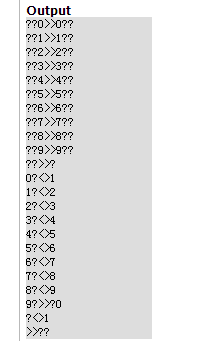
\includegraphics{algorithm.png}

如此无论对方输入什么,我都能得到答案。
\subsubsection{时空复杂度}
时间复杂度:$O(1)$

空间复杂度:$O(1)$
\newpage
\section{试题泛做6}
\subsection{Codeforces 294D Shaass and Painter Robot}
\subsubsection{题意}
给你一个$n$行$m$列的网格,一开始都是白色的,一个机器人在$(x,y)$处按某个方向(只会是东南、东北、西南、西北)走,撞到墙壁会按照光的反射定律行走下去。走的过程中会让走过的点变黑。

如果某个时刻网格黑白相间,他会停下来,问这个时刻。

如果永远停不下来输出$-1$。
\subsubsection{数据范围}
$n \le 10^5$
\subsubsection{题解}
根据光路可逆的话,模拟的时间复杂度是靠谱的,以及如何判断是否停不下来也只要多次经过起点就可以看做停不下来了。

关键在于如何判定是否黑白相间,这个我想了很久都没什么好思路。

据说如果边界上的所有点都黑白相间了,就能证明整个图已经黑白相间了。感觉好厉害的样子。
\subsubsection{时空复杂度}
时间复杂度:$O(n)$

空间复杂度:$O(n)$
\subsection{Codeforces 240F Torcoder}
\subsubsection{题意}
给你一个长度为$n$的字符串,有$m$个操作,每次操作$[l,r]$,为将$[l,r]$进行重排,得到一个字典序最小的回文串。如果无法得到则不进行。

求$m$次操作之后的字符串。
\subsubsection{数据范围}
$n,m \le 10^5$
\subsubsection{题解}
傻逼题吧。

用线段树维护每个区间里每个字符的出现次数,于是可以得到$[l,r]$里每个字符的出现次数。

接下来为了让字典序最小,我们贪心的摆进去就可以了。

摆进去的过程是一个区间赋值的任务,也能用线段树维护。
\subsubsection{时空复杂度}
时间复杂度:$O(26^2n \log n)$

空间复杂度:$O(26n)$
\subsection{USACO Open Contest 2011, Soldering}
\subsubsection{题意}
给你一棵树,要你用链覆盖,一条长度为$L$链的花费是$L^2$。

要求每条链的一个端点,要么是叶子,要么有另一条链过这个点且不是作为端点存在。

求最小花费。
\subsubsection{数据范围}
$n \le 50000$
\subsubsection{题解}
这题我有深深的罪恶感……我是暴力A掉的(题解好厉害的样子我没搞懂)。

那么先想想如何暴力$dp$吧。

设$dp[i][j]$为$i$的子树里,$i$连出去一条长度为$j$的链的最小花费。

然后对于$i$的儿子$x$,暴力枚举$x$连出去多少,只考虑有效状态(显然$x$连出去的不能超过$x$底下的最长链)。

看起来是$O(n^3)$的。

但其实这种$dp$方式有一个神奇的性质:任意两个点只会对他们的$lca$带来贡献。

也就是复杂度其实是$O(n^2)$的。

好,有了这个之后怎么做呢?

显然如果对于$dp[i][j]$和$dp[i][k]$,若有$j<k$且$dp[i][j] \le dp[i][k]$,那么$dp[i][k]$永远不会作为最优解被用到(因为这题是二次函数)。

那么我们可以每次把这样的$k$删掉,由于数据可能不是很好造,删掉了所有这种$k$之后,对于每个点的决策量就很少了。

接下来暴力转移发现竟然就A掉了,无论是官方数据还是清橙上的数据都能在比正解快的情况下跑出来。

正解似乎是维护凸包,每次转移的时候可以看做将两个凸包合并,使用启发式合并的方法做到只有$O(n \log n)$的插入次数,带插入的动态凸包可以用平衡树维护,总复杂度是$O(n \log^2 n)$的……只不过我不太理解的是这样子的话应该要做一个对每个点的坐标$+1$的操作,不知道应该怎么做到,所以就当是个大坑了。
\subsubsection{时空复杂度}
时间复杂度:$O(n^2)$

空间复杂度:$O(n)$
\subsection{Codeforces 332E Binary Key}
\subsubsection{题意}
假设$p,q$是两个字符串,$q$只含有$01$。

有这么一个算法。

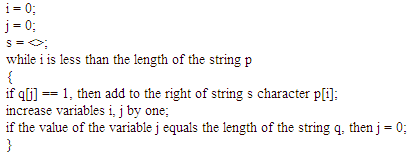
\includegraphics{code.png}

已知$p$和得到的字符串$|s|$以及$q$的长度$n$,要你求字典序最小的$q$。
\subsubsection{数据范围}
$n \le 2000$

$|p| \le 10^6,|s| \le 200$
\subsubsection{题解}
先枚举有几个$1$。假设有$m$个$1$。

从后往前一个个填$1$进去,第$i$位能填第$j$个$1$,当且仅当$p$串对应$i+kn$与$s$串对应的$j+km$是完全匹配的。

我们会发现,对于每个$i$,暴力检验的复杂度是$O(\frac{|p|}{n})$,要进行$n$次暴力,复杂度就是$O(|p|)$的。

所以总复杂度算下来不大,关键是我们能剪枝,跑的飞快的。
\subsubsection{时空复杂度}
时间复杂度:$O(n|p|)$

空间复杂度:$O(|p|)$
\subsection{Codeforces 293D Ksusha and Square}
\subsubsection{题意}
给你一个面积不等于$0$的凸多边形,随机选择两个\textbf{不同格点},以其连线为对角线做正方形,求正方形面积的期望值。
\subsubsection{数据范围}
$n \le 10^5$

坐标范围绝对值不超过$10^6$
\subsubsection{题解}
假设一个正方形的对角线长度是$L$,正方形的面积就是$\frac{L^2}{2}$。

我们关键要求的,应该是随机两点的对角线的平方的期望值。

两点间距离公式是$(x_1-x_2)^2+(y_1-y_2)^2$,我们可以把横纵坐标分开算,假设求随机两点的横坐标之差的平方的期望值。

$(x_1-x_2)^2=x_1^2-2x_1x_2+x_2^2$,可以对每一项分别计算,也就是要求所有点的横坐标之和与所有点的横坐标平方和。

注意到值域只有$2 \times 10^6$,我们可以暴力求出$x=k$时,这条竖线上的格点的横坐标之和与横坐标的平方和。

这样子就没了吧。
\subsubsection{时空复杂度}
时间复杂度:$O(n+10^6)$

空间复杂度:$O(n+10^6)$
\subsection{Codeforces 235C Cyclical Quest}
\subsubsection{题意}
给定字符串$s$和$n$个字符串$x_i$,对于每个$x_i$都要询问有多少$s$的连续子串是周期性同构于一个给定的字符串$x_i$。
\subsubsection{数据范围}
$|s| \le 10^6$

$\sum\limits_{i=1}^n |x_i| \le 10^6$
\subsubsection{题解}
像这种题,一般都要用到后缀数据结构。

而如果数据量达到了$10^6$的级别,后缀数组则是无法胜任的。

我们可以用后缀自动机来实现这题,后缀自动机的相关知识相当繁琐,所以略去不提。

构造出后缀自动机后,就能在线的回答询问。对每组询问,把询问的串在后缀自动机上跑一下就行了。

由于后缀自动机的各种性质,它可以轻松处理这道题目。
\subsubsection{时空复杂度}
时间复杂度:$O(26|s|+\sum\limits_{i=1}^n |x_i|)$

空间复杂度:$O(26|s|)$
\subsection{USACO Open Contest 2013, Photo}
\subsubsection{题意}
有$n$头奶牛排成一排,标号为$1 \sim n$。小明拍了$m$张照片,照片$i$包含了从$a_i$到$b_i$的奶牛,每张照片中恰有一头奶牛有斑点。问至多有多少头奶牛有斑点。
\subsubsection{数据范围}
$n \le 2 \times 10^5$

$m \le 10^5$
\subsubsection{题解}
一头牛可以有斑点,当且仅当它和前一头有斑点的牛之间没有空照片,以及它们不在同一张照片里。

令$f_i$表示第$i$头牛有斑点时,前$i$头牛中最多有斑点的牛数。

计算$f_i$时,枚举前面一个有斑点的牛$j$,拿$f_j+1$转移。

$j$需要满足什么条件呢?就需要不存在一张照片恰好包含了$i,j$,也不存在一张照片被$[j,i]$包含。

我们可以预处理$l_i$表示右边界比$i$小的照片左边界最大在哪里,$r_i$表示右边界比$i$大的照片做边界最小在哪里。

就需要$l_i \le j < r_i$。

预处理了$l,r$后,能用线段树优化$dp$。
\subsubsection{时空复杂度}
时间复杂度:$O(n \log n)$

空间复杂度:$O(n)$
\subsection{Codeforces 338E Optimize!}
\subsubsection{题意}
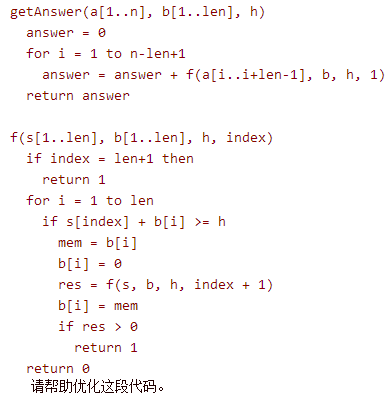
\includegraphics{Optimize!.png}
\subsubsection{数据范围}
$len \le n \le 1.5 \times 10^5$

$a_i,b_i,h \le 10^9$
\subsubsection{题解}
显然的,如果要判定数组$a$能否与数组$b$做到一一匹配且两两之和大于等于$h$,那么一个有效的判定方法就是贪心,即将$b$从小到大排序后,对$a$的每个数,贪心的找$b$里面最小的能和他匹配的数。

证明可以用霍尔定理证明。

我们把序列每$\sqrt{n}$分成一块,在块$[l,r]$内的每个$i$,判定$[i,i+len-1]$是否能与$b$匹配。

贪心的那个方法是可以把$a$按任意顺序来贪心的,我们发现如果$len \ge \sqrt{n}$的话,我们先对$[r+1,i+len-1]$贪心,那么对于任意的$i \in [l,r]$,没有处理好的就只有$O(\sqrt{n})$个了。我们平方的贪心。这样子算下来是$O(n\sqrt{n})$的。

如果$len < \sqrt{n}$怎么办呢?直接根据题意模拟即可,我写了个$O(n\sqrt{n}\log n)$的贪心。
\subsubsection{时空复杂度}
时间复杂度:$O(n\sqrt{n}\log n)$

空间复杂度:$O(n)$
\subsection{USACO December Contest 2007, Best Cow Line}
\subsubsection{题意}
有$n$头奶牛,每个奶牛身上有个字符,你每次能取出第一个奶牛,也能取出最后一个奶牛,要取完奶牛得到一个序列,字典序最小。
\subsubsection{数据范围}
$n \le 30000$
\subsubsection{题解}
假设要处理$[l,r]$。

首先,若$a_l \neq a_r$,则能通过$a_l,a_r$的大小关系确定,变成一个递归的子问题,让规模减小$1$。

那么现在考虑$a_l=a_r$的问题,最优解可不可能只有先取$a_l$,再取$a_r$,再取$a_{l+1}$呢?不可能,因为这样的话和先取$a_r$,再取$a_l$是没有区别的。

换句话说,如果取了$a_l$后的最优解的第一步不是$a_{l+1}$,那么我最开始取$a_l$还是$a_r$都无关紧要。

同理,如果最优解是取$a_l,a_{l+1},a_{l+2},a_r$,而$a_{l+1}=a_{r-1},a_{l+2}=a_{r-2}$,则最开始取$a_l$还是$a_r$也是无关紧要的。

这么推理下去,我们可以得到这样的贪心方法:找到最小的$k$,满足$a_{l+k} \neq a_{r-k}$,则通过比较两者大小,$a_{l+k}<a_{r-k}$就先取$a_l$,否则先取$a_r$。

那么如何得到这个$k$呢?就等价于原串与翻转后的串的一个LCP的问题,可以用二分+哈希解决。
\subsubsection{时空复杂度}
时间复杂度:$O(n \log n)$

空间复杂度:$O(n)$
\subsection{Google Code Jam World Final 2014 C Symmetric Trees}
\subsubsection{题意}
给你一棵树,每个点都有一个颜色。

要你把这棵树画在平面上,边不相交,点的位置不能相同,画出来的图形关于$y$轴对称。
\subsubsection{数据范围}
$n \le 10^4$
\subsubsection{题解}
首先一个前置技能是判断两棵树是否可以做到完全对称。

说白了就是带颜色的情况下的树同构问题。

这个可以用哈希的方法,求出树的最小表示,从而解决问题。

有了这个武器,我们先像树形dp一样,先让$1$号点当根看做有根树,求出每个点的子树的哈希值,往上走的哈希值。

然后可以递推$can_i$表示以$i$为根的子树能不能画上去,并且要求不存在一个在$y$轴上的点,他有两个儿子在$y$轴上。

这个$can_i$是可以像树形$dp$一样递推出来的。

分三种情况考虑:没有点在$y$轴上,没有一个点有两个儿子在$y$轴上,恰好有一个点有两个儿子在$y$轴上。

对三种情况分别利用这几个数组来考虑就可以了。
\subsubsection{时空复杂度}
时间复杂度:$O(n \log n)$

空间复杂度:$O(n)$
\subsection{Codeforces 251E Tree and table}
\subsubsection{题意}
有一棵$2n$个点的数。

你要填一个$2$行$n$列的表格,表格里面是一个$1 \sim 2n$的排列。

要求若树上的$i,j$相邻,则表格里他们也要相邻(四联通)。

求方案数。
\subsubsection{数据范围}
$n \le 10^5$
\subsubsection{题解}
相当繁琐的分情况讨论dp。

显然每个点的度数不会超过$3$。

如果没有度数等于$3$的点,是可以推公式的。不妨默认存在度数等于$3$的点,将他提根。

那么他的三个点就会分别在他的左边、下边、右边处。可以$3!$爆枚。

爆枚之后分情况讨论会发现,我们需要计算两种东西$g(a,b)$和$dp[i]$,分别表示$a,b$两棵子树填到表格里面,$a$在左上$b$在左下的方案数;以及$i$的子树填到表格里$i$在左上的方案数。

很容易发现已知了$dp$后,就知道$g$了。

我们考虑计算$dp[i]$。

显然要求$i$的两棵子树中至多有一棵存在度数为$3$的点。

先特判掉一些情况。

找到离$i$最近的度数为$3$的点。

如果$i$的度数为$1$,可以写出$dp$方程,大概就是说,假设$i$的左儿子度数也是$1$,就是$dp[i$的左儿子的左儿子$]$。否则的话,$i$的左儿子只能放在$i$的右边,然后分情况讨论一下,$i$的左儿子的一个儿子放在下面,一个儿子放在右边,然后继续讨论是能算出来的……

如果$i$的度数不是$2$的话,沿用上面的做法会超级难写,问了别人之后得知有这么一个简便的做法:直接利用$g$函数能求出来!

这样子的话转移就没问题了,然后$g$会用到的有效状态是$O(n)$的。
\subsubsection{时空复杂度}
时间复杂度:$O(n)$

空间复杂度:$O(n)$
\subsection{Codeforces 249E Endless Matrix}
\subsubsection{题意}
有一个无限大矩阵,他的前六行六列矩阵长这样

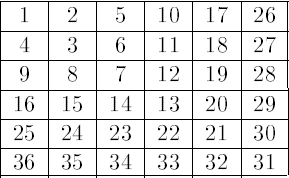
\includegraphics{matrix.png}

求一个以$(x_1,y_1)$为左上角$(x_2,y_2)$为右下角的子矩形的所有数字的和的后$10$位。

如果答案超过了$10$位,前面要输三个点。

$T$组数据。
\subsubsection{数据范围}
$T \le 10^4$

$x_1,y_1,x_2,y_2 \le 10^9$
\subsubsection{题解}
关于$a \times b$对一个十位数取模的方法可以用long double做到$O(1)$计算的技巧不再赘述。

然后为了判断他是不是超过了$10$位,可以再对$10^{10}-1$取模。

为了计算一个矩形的权值和,可以用容斥原理,转化为一个$(1,1)$为左上角$(n,m)$为右下角的矩形的权值和。

观察发现,令$x=\min(n,m)$,前$x$行$x$列的和是可以$O(1)$的,正好就是$1 \sim x^2$的和,能用等差数列求和公式计算。

假设$n<m$,就会多出一块小矩形,小矩形每一列是等差数列,每一行是差后等差数列。写出公式后可以$O(1)$计算。

假设$m<n$,也会多出一块小矩形,小矩形每一行是等差数列,每一列是差后等差数列。写出公式后可以$O(1)$计算。
\subsubsection{时空复杂度}
时间复杂度:$O(T)$

空间复杂度:$O(1)$
\newpage
\section{试题泛做7}
\subsection{USACO November Contest 2012, Balanced Trees}
\subsubsection{题意}
给你一棵树,每个点上有个标记是“(”或者“)”。

要你找一个点对$(u,v)$,满足$(u,v)$路径上的括号能够构成合法括号序列,并且最大化层数。

所谓层数,指的是将左括号看做$1$,右括号看做$-1$的情况下,最大前缀和。
\subsubsection{数据范围}
$n \le 40000$
\subsubsection{题解}
看到是点对问题,就会想到树分治。

把左括号看做$1$,右括号看做$-1$,一个合法括号序列要满足最小前缀大于等于$0$,长度和等于$0$。

处理经过重心的路径的时候,我们要做的就是查询最小前缀和大于等于某个值的和等于某个值的括号序列的最大前缀和。

用线段树维护即可。
\subsubsection{时空复杂度}
时间复杂度:$O(n \log^2 n)$

空间复杂度:$O(n \log n)$
\subsection{Codeforces 285E Positions in Permutations}
\subsubsection{题意}
称一个$1 \sim n$的排列的完美数为有多少个$i$满足$|P_i-i|=1$。

求有多少个长度为$n$的完美数恰好为$m$的排列。
\subsubsection{数据范围}
$n \le 1000$
\subsubsection{题解}
容斥原理,转化为至少$i$个的。

我们考虑$dp[i][j]$为前$i$个数填了$j$个完美,那么转移应该是分填$i+1,i-1$与不让完美数增加三种情况讨论。

但是如果填$i-1$,就会涉及到$i-1$有没有被前面那个人填到过的问题。我们可以多记几维,$dp[i][j][0/1][0/1]$表示前$i$个数有至少$j$个完美,$P_{i-1}$是否等于$i$,$P_i$是否等于$i+1$。

这样子转移就没问题了。

我们就知道填了$i$个完美位置的排列数$ans_i$,那么排列数是不是$ans_i \times (n-i)!$呢?其实不是的,因为有重复计数。

我们会发现一个完美数为$i$的排列会给一个完美数为$j$的排列带来${i \choose j}$的冗余贡献,预处理组合数减掉就行了。
\subsubsection{时空复杂度}
时间复杂度:$O(n^2)$

空间复杂度:$O(n^2)$
\subsection{Codeforces 295D Greg and Caves}
\subsubsection{题意}
符合以下条件的黑白矩阵合法:

存在一个区间$[L,R](1 \le L \le R \le n)$,使得上至行$L$、下至行$R$,每一行都恰有$2$个黑点,而其他列只有白点。

定义:【中间白点是指同一行处在$2$个黑点之间的白点,$left_i$表示第$i$行靠左边的黑点所在列,$right_i$表示靠右边的黑点所在列】

存在一个行号$t \in [L,R]$,使得:
\begin{enumerate}
\item 对于任意$L \le i \le j \le t$,第$i$行的任意列的中间白点,第$j$行的同一列都是中间白点。且$left_i \ge left_j,right_i \le right_j$
\item 对于任意$t \le i \le j \le R$,第$j$行的任意列的中间白点,第$i$行的同一列都是中间白点。且$left_i \le left_j,right_i \ge right_j$
\end{enumerate}

求合法矩阵数。
\subsubsection{数据范围}
$n,m \le 2000$
\subsubsection{题解}
简单的$dp$就行了。

我们不关心$t$行的左右边界,只关心$t$行的长度。

$dp[i][j]$表示到了第$i$行,底边长度为$j$的左边界单调递减右边界单调递增的方案数。

转移的话,$dp[i][j]=\sum\limits_{k=2}^j dp[i-1][k](j-k+1)$,我们很容易优化他。

$O(n^2)$的预处理出$dp$数组之后,我们暴力枚举第$t$行的长度就行了。但是如果第$t$行与第$t+1$行长度相同,会出现重复计算。我们不妨强制要求第$t+1$行长度小于第$t$行的长度即可。
\subsubsection{时空复杂度}
时间复杂度:$O(n^2)$

空间复杂度:$O(n^2)$
\subsection{Google Code Jam World Final 2010 A Letter Stamper*}
\subsubsection{题意}
你要打印一个\textbf{只含有字符ABC}的字符串$S$。

你的打印机比较弱,他是一个栈式打印机,支持以下三种操作
\begin{enumerate}
\item 插入一个字符到栈顶
\item 弹出栈顶字符
\item 打印栈顶字符
\end{enumerate}

要你用最少的操作次数打印字符串。
\subsubsection{数据范围}
令$n$代表$S$的长度,$n \le 2000$
\subsubsection{题解}
$O(n^3)$的$dp$是很显然的,就是像石子合并一样做就行了。

但由于决策没有性质,无法用四边形不等式优化。

我们只能从只有三种字符和分析打印策略入手。

一个显然的事实是说,最优解的栈在任何时刻都不会有相邻的两个字符相同。

仔细分析,其实我们还能得到这样的兴致:最优解的栈在任何时刻都不会出现距离差为$2$的两个字符相同,即不会有形如$ABA$的子串。

这样的话,假设栈前$3$个字母定下来了,栈后面的每个字母就知道了。我们能用二元组$($长度,前三个字母$)$来表示一个栈。

这样的话,就能$dp$了,我们强行把栈设入状态,$dp[i][L][a][b][c]$表示前$i$个字符,长度是$L$,前三个字母用$a,b,c$表示。转移显然。
\subsubsection{时空复杂度}
时间复杂度:$O(n^2)$

空间复杂度:$O(n)$
\subsection{USACO January Contest 2009, Safe Travel}
\subsubsection{题意}
给你一个$n$个点$m$条边的无向图,\textbf{保证从点$1$到任何一个点的最短路径唯一}。

求对于每个点$i$,删去$1$到$i$的最短路径的最后一条边后$1$到$i$的最短路径是多少。
\subsubsection{数据范围}
$n \le 10^5,m \le 2 \times 10^5$
\subsubsection{题解}
从点$1$开始跑一遍Dijkstra,能得到一棵最短路径树。不在最短路径树上的边称之为非树边,在的边称之为树边。称$dis_u$为$1$到$u$的最短路径。

求到一个点$v$的最短路径,假设$u$是$v$的父亲,那就是删去了边$(u,v)$一定是$1$沿着树边走到点$a$($a$不在$v$的子树内),然后$a$走一条非树边走到$b$($b$在$v$的子树内),然后$b$再沿着树边走到$v$。

也就是要最小化式子$dis_a+len(a,b)+dis_b-dis_v$,其中$a$不在$v$的子树,$b$在$v$的子树。

子树可以先DFS遍历一遍,映射成DFS序的一段区间,假设是$[l,r]$。$pos_i$表示$i$在DFS序中的位置。

要求得就是最小化$dis_a+len(a,b)+dis_b(pos_a \not \in [l,r],pos_b \in [l,r])$。

由于这种$(a,b)$是$O(m)$的,可以存下来,看做在二维平面上的点$(pos_a,pos_b)$上打了一个$dis_a+len(a,b)+dis_b$的标记,要求支持查询$pos_a$在某个范围$pos_b$在某个范围的最值。

把所有的$(a,b)$按$pos_a$排序,可以利用单调性减少一维,问题就只有一维了。要支持的是单点赋值和区间最值查询,可用线段树实现。
\subsubsection{时空复杂度}
时间复杂度:$O((n+m) \log n)$

空间复杂度:$O(n+m)$
\subsection{Codeforces 257E Greedy Elevator}
\subsubsection{题意}
要你模拟一个电梯的过程。

总共有$n$个事件,第$i$个事件表示时刻$t_i$会有一个人在$a_i$等电梯想去$b_i$。

电梯在时刻$0$是在第一层,总共有$m$层。

走进走出电梯是瞬间的。

每一秒,如果没有人在电梯里,也没有人在等电梯,电梯会停住。

否则,如果电梯在楼层$x$,我们定义$p_{up}$表示电梯中要到编号比$x$大的楼层的人和当前时刻$t$在编号比$x$大的楼层等电梯的人的总数,$p_{down}$表示电梯中要到编号比$x$小的楼层的人和当前时刻$t$在编号比$x$小的楼层等电梯的人的总数。如果$p_{up} \ge p_{down}$,那么电梯在时刻$t+1$会到楼层$x+1$,否则电梯会到楼层$x-1$。

输出每个人到达目的地的时刻。
\subsubsection{数据范围}
$n,m \le 10^5$
\subsubsection{题解}
一道裸裸的数据结构模拟题。

可以用平衡树或堆维护时间点。

此外每次要能查询$p_{up}$和$p_{down}$,我们可以看做进来一个人时在$a_i$处减$1$,$b_i$处加$1$;而有人在等电梯时则是在$a_i$处加$1$。

这样的话就只要查询区间和。能用树状数组维护。
\subsubsection{时空复杂度}
时间复杂度:$O(n \log n)$

空间复杂度:$O(n)$
\subsection{Codeforces 316E3 Summer Homework}
\subsubsection{题意}
给你一个长度为$n$的数列,$m$个操作,每个操作会是如下三种形式之一:

\begin{enumerate}
\item 输入$x,v$,将$a_x$赋值成$v$。
\item 输入$l,r$,询问$\sum\limits_{i=l}^r a_i f_{i-l}$,$f_i$代表斐波那契数列第$i$项。
\item 输入$l,r,d$,要去给区间$[l,r]$每个数加上$d$。
\end{enumerate}
\subsubsection{数据范围}
$n,m \le 200000$
\subsubsection{题解}
$Fib$数一般用矩阵形式或者二次剩余来写成一个数的若干次方,这题模数没有二次剩余,我们考虑用矩阵来表示。

$Fib$的转移矩阵的若干次方的右上角就代表对应的斐波那契数,矩阵还可以相加。

用线段树维护,一个节点存区间$[l,r]$的$\sum\limits_{i=l}^r a_i F^{i-l}$,$F$代表$Fib$转移矩阵。

再预处理$Fib$矩阵的若干次方就能完全信息合并,可以做前两问了。

至于第三问,我们像普通的区间加一样打标记,并且预处理$Fib$矩阵的若干次方数组的前缀和就行了。
\subsubsection{时空复杂度}
时间复杂度:$O((n+m) \log n)$

空间复杂度:$O(n)$
\subsection{Codeforces 356E Xenia and String Problem}
\subsubsection{题意}
如果字符串$s$满足如下条件,称他为Gray串。

\begin{enumerate}
\item $|s|$是奇数。
\item 正中间的那个字符只出现了一次。
\item $|s|=1$或者左边一半等于右边一半且也是Gray串。
\end{enumerate}

一个串的美丽值是所有Gray子串的长度的平方和。

你能修改一个字符,最大化修改后的串的美丽值。
\subsubsection{数据范围}
$|s| \le 10^5$
\subsubsection{题解}
显然Gray串数目甚至连长度为$2^k+1$的串数目都是$O(n \log n)$级别的。

先用倍增表预处理出$[i,i+2^j-1]$的哈希值。也能预处理从而$O(1)$的到原串的某个子串是不是Gray串。

先计算原串的美丽值,枚举某一位换成某个字符,计算变化量。

枚举所有以当前字符为中心的长度为$2^k-1$的Gray串,然后对于一个Gray串$[l,r]$,来看$[l,(r+1)+(r-l+1)]$是不是Gray串,$[(l-1)-(r-l+1),r]$是不是Gray串,如果是的话递归进行。

感觉这样子的话,一个长度为$2^k+1$的串顶多被考虑$26+2$次(他只有在是Gray串的时候才会被考虑),均摊复杂度应该是靠谱的。
\subsubsection{时空复杂度}
时间复杂度:$O(26n \log n)$

空间复杂度:$O(26n + n \log n)$
\subsection{Codeforces 297E Mystic Carvings*}
\subsubsection{题意}
一个长度为$2n$的圆环上,有$n$条弦。每条弦的端点互不相同。

如果我选了$3$条弦,称这种选择合法的话,当且仅当对于每条弦的距离相等;而一条弦$(a,b)$的距离的定义是从$a$走到$b$最少经过另外两个弦里的几个弦。

求合法方案数。
\subsubsection{数据范围}
$n \le 10^5$
\subsubsection{题解}
关键在于分析出三条弦的相交情况,这是比较麻烦的。

看题解后知道,相交情况只有$5$种。

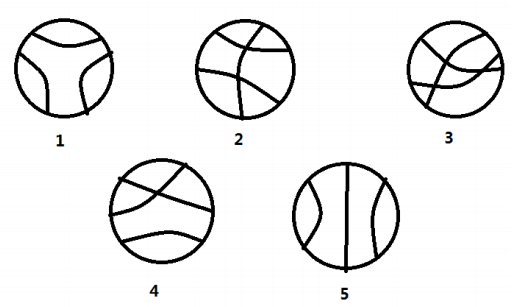
\includegraphics{carve.png}

分析之后,情况$1,3$即为所求,但这个不好算,不妨补集转化,变成求情况$2,4,5$,然后用${n \choose 3}$减去他。

用离线树状数组的技巧,我们能快速计算出,一条弦与几个弦相交,以及一条弦包含了几条弦。

于是情况$5$就好算了。至于情况$2,4$,我们能把他们合起来——统计有多少这样的局面:弦$A$与弦$B$相交,与弦$C$不相交。

我们可以惊喜的发现,这种局面的个数正好是情况$2$加上情况$4$的两倍。
\subsubsection{时空复杂度}
时间复杂度:$O(n \log n)$

空间复杂度:$O(n)$
\subsection{Codeforces 360E Levko and Game}
\subsubsection{题意}
给你一个$n$个点$m$条边的图,有两个人一个人从$s_1$要走到$t_1$,一个人从$s_2$要走到$t_2$,有$k$条边你可以把边权赋值为$[L_i,R_i]$中的一个值,要你通过改边权,让第一个人的最短路比第二个人的最短路短。
\subsubsection{数据范围}
$n,m \le 10^4$

$k \le 100$
\subsubsection{题解}
贪心的来想,一条边肯定要么希望他变成$L_i$以使得对自己有利,要么希望变成$R_i$以使得对对方有害。

通过迭代的方法来实现。每次重新跑Dijkstra。把离对方更近的边增大,离自己更近的边减少。

感性的理解迭代次数是很小的。后来看了下官方题解,似乎是可以证明只要把离自己更近的边减少就能得到最优解的,没有很想明白证明。
\subsubsection{时空复杂度}
时间复杂度:$O((n+m)k \log n)$

空间复杂度:$O(n+m)$
\subsection{USACO March Contest 2012, Cows in a Skyscrape}
\subsubsection{题意}
有$n$个奶牛,第$i$头奶牛重$w_i$,有一个能承受$m$重量的电梯,你要把奶牛全部运下去,问最少运几次。
\subsubsection{数据范围}
$n \le 18$
\subsubsection{题解}
朴素的$dp$方法是设$dp[S]$表示把集合$S$运下去的最小次数,通过枚举子集来转移,复杂度是$O(3^n)$的,不再赘述。

听说卡常数可以A,有点可怕。

官方做法是$O(2^nn^2)$的。

令$dp[i][S]$为给集合$S$运$i$次,最多能运走多少重量。

转移是这样的。

令$sum[S]$为集合$S$的总重量。

一方面,如果求出了$dp[i]$,那么对于任意$S$,若$sum[S]-dp[i][S] \le m$,有$dp[i+1][S]=sum[S]$。

另一方面,对于任意的$S' \in S$,有$dp[i][S] \ge dp[i][S']$。

用这种方式来$dp$,第一种情况当然是$O(2^nn^2)$的,第二种情况我们只需要枚举所有$S$,取$dp[i][S \oplus 2^k]$(要求集合$S$的第$k$位是$1$)来更新就好了,因为其余的子集都是枚举到的这些东西的子集,不会更优。
\subsubsection{时空复杂度}
时间复杂度:$O(2^nn^2)$

空间复杂度:$O(2^nn)$
\subsection{Codeforces 303E Random Ranking}
\subsubsection{题意}
有一次考试,这场考试有$n$个考生。

你知道第$i$个考生的得分范围是$[L_i,R_i]$(得分可以是实数),现在你要预测每个考生得到任何排名的概率。

提示:无需考虑多个考生有相同分数的情况。
\subsubsection{数据范围}
$n \le 80$
\subsubsection{题解}
离散化后,有$O(n)$个时间段,我们可以一段段计算。

枚举一个人,枚举这个时间段,一个比较显然的$dp$是说,将其他与这个时间段相交的区间取出来。

设$dp[i][j]$为前$i$个人有$j$个比他分数低的概率不好转移,可以设成是一个多项式。假设当前区间是$[a,b]$,一个人的得分区间是$[c,d]$,那么如果$c \le a$,这个人分数比他低的概率就是$\frac{x-c}{d-c}$了。而比他大的概率则是$\frac{d-x}{d-c}$。

用类似于01背包的方法$dp$,可以对每一段都求出最后的函数,定积分一下,这样子理论上是可以的,但是很不爽的是和标程有一点精度误差……所以就只能按照标程的方法来$dp$。

标程是这样的,注意到这么一个事实是说,如果有$k$个其他人都分布在区间$[a,b]$,那么我在$[a,b]$的情况下,得到任何一名的概率都应该是$\frac{1}{k+1}$。有了这个思路,我们能直接$dp$。设$dp[i][j]$为有$i$个人分数比他所在区间低,$j$个人分数和他所在区间一样,转移是显然的。

接下来,$dp[i][j]$能对他排在$i+1,i+2,i+3,\cdots,i+j+1$都带来$\frac{dp[i][j]}{j+1}$的贡献,可以用差分的方法实现。

最后复杂度是一样的,但是这样子能过。
\subsubsection{时空复杂度}
时间复杂度:$O(n^5)$

空间复杂度:$O(n^2)$
\newpage
\section{试题泛做8}
\subsection{USACO December Contest 2005, Cow Patterns}
\subsubsection{题意}
给你两个字符串$A,B$,要你求$A$能匹配多少次$B$。$A,B$长度分别为$n,m$。字符集大小为$S$。

两个字符串匹配本来指的是长度相同且各个位相同;我们这里改变一下,称两个字符串匹配,当且仅当他们按大小离散化后得到的字符串相同(也就是对应位置上的数的$rank$是一样的)。
\subsubsection{数据范围}
$n \le 10^5,m \le 25000$

$S \le 25$
\subsubsection{题解}
KMP的一个扩展。

假设本来已经匹配了串$S1,S2$

现在给$S1$加入字符$a_1$,$S2$加入字符$a_2$,要求$S_1$里小于$a_1$的数和$S_2$里小于$a_2$的数个数相同;$S_1$里等于$a_1$的数和$S_2$里等于$a_2$的数个数相同。

用前缀和预处理可以$O(1)$进行判定。

接下来把这种新的定义套入以前的KMP算法即可。
\subsubsection{时空复杂度}
时间复杂度:$O((n+m)S)$

空间复杂度:$O((n+m)S)$
\subsection{Codeforces 331D3 Escaping on Beaveractor}
\subsubsection{题意}
平面上有$n$个箭头。箭头会指向东西南北的一个方向。

如果你走到了一个箭头,你就会沿着箭头的方向走下去。

有$m$个询问,每个询问是如果某人在某个点$(x_i,y_i)$向某个方向$d_i$走去(方向也只可能是东西南北),$t_i$秒后他会在哪。如果$t_i$秒时他在以$(0,0)$为左下角$(b,b)$为右上角的正方形外,输出他最后一次在正方形内的坐标。
\subsubsection{数据范围}
$n \le 10^5$

$m \le 10^5$
\subsubsection{题解}
属于一眼知道做法写的人想死的代码题……

首先,能用扫描线的方法,求出走到每个箭头后,会走到的下一个箭头。

同样的,能用扫描线的方法,求出每个人会走到的第一个箭头。

弄出了这个之后,建立倍增表,像LCA一样的跳一跳。

神奇的事情是我一不小心写了将近$10K$的代码量,称为清橙上通过这题的人里代码最长的一个(真心给$2K$写出来的跪傻了)
\subsubsection{时空复杂度}
时间复杂度:$O(n \log n)$

空间复杂度:$O(n \log n)$
\subsection{Codeforces 293B Distinct Paths}
\subsubsection{题意}
有一个$n$行$m$列的木板,一些块已经被涂上给出的$k$种颜色中的一种。

你需要把每个没涂色的块涂色,使得从左上角到右下角的每条路径都不会经过两个颜色一样的块。路径只能向右或向下走。
\subsubsection{数据范围}
$n,m \le 1000$

$k \le 10$
\subsubsection{题解}
首先,若$n+m-1 > k$,显然无解,特判即可。

这样一来,就有$n+m-1 \le k$了。

不妨设$n>m$,就有$m \le 5$,考虑状压dp。

按格转移,记录每个颜色最近的出现位置,为了保证合法,状态数很稀疏。
\subsubsection{时空复杂度}
时间复杂度:$O(nmS)$,$S$代表状态数,是比较小的。

空间复杂度:$O(nm+S)$。
\subsection{USACO January Contest 2007, Cow Schul}
小美考了$n$场考试,第$i$场考试满分为$P_i$,她的得分是$T_i$。

老师为了帮她作弊,会把得分比例最低的$D$份试卷去掉,得分比例$F_i=\frac{T_i}{P_i}$

最后计算总成绩$G=\frac{\sum T_i}{\sum P_i}$。

不过小美却发现,对于有些$D$,她可以删掉另外的$D$份试卷,比老师算出来的得分更高。

请找出这些$D$。
\subsubsection{数据范围}
$n \le 50000$
\subsubsection{题解}
因为是比例,很容易想到类似于分数规划的思想。

若$\frac{\sum T_i}{\sum P_i} \ge \lambda$,则有$\sum T_i \ge \sum P_i \lambda$。

枚举$D$,令$\lambda$为此时老师的得分,是可以算的。我们要删去$D$份卷子后满足$\sum T_i \ge P_i \lambda$,这个不好办。

但事实上问题可以简化:如果有办法更优,就一定存在一个办法是把老师的一份卷子替换成我的一份卷子。

再转化一下,就是把老师的最大的卷子替换成我的最小的卷子。

这时,问题变成了:支持动态插入一条直线,询问与$x=k$这条直线的最低/最高交点的坐标!

官方题解似乎利用了这题的特殊性质,给出了一种非常神奇的做法,我没有看懂。事实上这种问题都是用通用做法的,比如平衡树维护半平面交之类的。

我使用了陈丹琦分治。大家都知道,如果$n$条直线的极角有单调性,就能用一个单调栈做到$O(n)$处理。我用陈丹琦分治,先对左边处理,再对右边处理,用归并的方法将两边按极角排序后再处理,代码量相对而言大一点。
\subsubsection{时空复杂度}
时间复杂度:$O(n \log n)$

空间复杂度:$O(n)$
\subsection{Codeforces 316F3 Suns and Rays}
\subsubsection{题意}
给你一张图,他用一个$n$行$m$列的$01$矩阵表示,$0$表示背景,$1$表示图形。

上面有若干个太阳,太阳带一些光线。太阳是椭圆形,光线是一条连接在椭圆上的线段。如下面几幅图。


\includegraphics{SunRay1.png}

\includegraphics{SunRay2.png}

\includegraphics{SunRay3.png}

要你进行图像识别,判定有几个太阳,以及每个太阳上有几个光线。
\subsubsection{数据范围}
$n,m \le 1600$

没有两个太阳有共同点。

射线的宽度为3像素。

太阳的轴的长度将介于40和200像素。

没有两条射线相交。

所有射线的长度将在10和30像素。

肉眼可辨。
\subsubsection{题解}
一道比较简单的图像识别题。

几个太阳只需要FloodFill就行了,关键是光线的问题。

我们试图寻找光线射到的最远的点。

太阳上的点周围的点会比较稠密,而光线因为宽为$3$,所以周围的点会很稀疏。而如果是光线最远的点的话,周围的点就更稀疏了。

计算以每个点为中心,$11$为边长的正方形内有几个点,就能很明显的区分出圆上的点和光线上的点了。将光线上的点加进去。

可这样的话,一道光线很可能被加入多个点。

为了解决这个问题,我们需要进行如下操作:对于两个点$A,B$,如果$A$在$B$左边或者正下方,他们在同一个光线上,则删除$B$。

具体来讲,如果两个点曼哈顿距离小于等于$30$,我们就让点$A$向点$B$走。注意不是看存不存在一条路径,而是直接贪心的走,即如果横坐标不相等,就让$A$向右走一步,否则向上(或者向下)走一步。如果这种走法走得到的话,估计就在一条光线上了。

由于是以曼哈顿距离小于等于$30$为前提的,所以判定的复杂度不会太高。
\subsubsection{时空复杂度}
时间复杂度:$O(n^2)$

空间复杂度:$O(n^2)$
\subsection{Codeforces 354D Transferring Pyramid}
\subsubsection{题意}
一个$n$层的金字塔,你能进行两种操作。

\begin{enumerate}
\item 给某个点染色,代价是$3$。
\item 画一个子三角形,底边必须是金字塔的底边,代价是点数+$2$。
\end{enumerate}

现在有$m$个黑点。要你覆盖所有黑点。
\subsubsection{数据范围}
$n,m \le 10^5$
\subsubsection{题解}
首先三角形是不会存在包含的。

为了方便,想象成他是等腰直角三角形好了。

考虑子三角形,会是以某个点为直角顶点的三角形,而且这个点为直角顶点只会弄一个三角形出来(因为互不包含)。

这样子就能写出暴力dp了。但直接做是$O(n^2)$的。

观察发现,答案不会超过$3m$,所以一个三角形的长度最多是$O(\sqrt{m})$的,这样的话就降低了dp的复杂度。
\subsubsection{时空复杂度}
时间复杂度:$O(n\sqrt{n})$

空间复杂度:$O(n\sqrt{n})$
\subsection{USACO March Contest 2013, Hill Walk}
\subsubsection{题意}
这里有$n$座山。每座山用一条从$(x_1,y_1)$到$(x_2,y_2)$的线段来描述,$x_1<x_2,y_1<y_2$。线段严格不相交。

奶牛贝茜从第一座山的位置开始。当贝茜在某座山上时,她会一直爬到这座山的尽头,然后从边上跳下来。如果她落在另一座小山上,她就会继续爬那一座山;否则结束。

请计算出贝茜走过的山的总数。
\subsubsection{数据范围}
$n \le 10^5$
\subsubsection{题解}
建立线段树。

由于互不相交,每个线段能拆成线段树上若干个点,我们他们都暴力存进去。

接下来把线段树每个点对应的区间都排序。

查询只要在线段树上的这些点都找一下前驱即可。因为区间排好了序,可以二分查找。
\subsubsection{时空复杂度}
时间复杂度:$O(n \log^2 n)$

空间复杂度:$O(n \log n)$
\subsection{Codeforces 288E Polo the Penguin and Lucky Numbers}
\subsubsection{题意}
称一个数是幸运数当且仅当他只含有$4$或者$7$。

给你两个数$l,r$,要求你把$[l,r]$的所有幸运数找出来按大小排序,假设记作$a_1,a_2,\cdots,a_n$,求$\prod\limits_{i=1}^{n-1} a_ia_{i+1}$。
\subsubsection{数据范围}
$1 \le l \le r \le 10^{10000}$
\subsubsection{题解}
转化为小于等于$r$的答案。

思考一个数的后继是什么。

假设一个数末尾有$x$个$7$,他的下一个数是把所有$7$变成$4$,把最后一个$4$变成$7$。

这样的话,假设这个$477\ldots 7$是$v_1$,这个$744\ldots 4$是$v_2$,前面的数字是$a$,长度是$m$,贡献就是$(10^ma+v_1)(10^ma+v_2)=10^{2m}a^2+10^m(v_1+v_2)a+v_1v_2$。

我们发现要求的是前若干位满足不超过$r$且是$4$或者$7$的情况下,他们的平方和、和、个数。

用数位dp处理即可。
\subsubsection{时空复杂度}
令$n=\lg(r)$

时间复杂度:$O(n)$

空间复杂度:$O(n)$
\subsection{Codeforces 258D Little Elephant and Broken Sorting}
\subsubsection{题意}
有一个$1 \sim n$的排列,会进行$m$次操作,操作为交换$a,b$。每次操作都有$50\%$的概率进行。

求进行$m$次操作以后的期望逆序对个数。
\subsubsection{数据范围}
$n,m \le 1000$
\subsubsection{题解}
简单期望题。

和的期望等于期望的和。

令$dp[a][b]$为第$i$个位置比第$j$个位置大的概率。

进行一次操作后,会改变$O(n)$个dp值,暴力重新计算一下就行了。
\subsubsection{时空复杂度}
时间复杂度:$O(n(n+m))$

空间复杂度:$O(n^2)$
\subsection{USACO January Contest 2012,Cow Run}
\subsubsection{题意}
奶牛们在长度为$m$的环形轨道上从相同的位置开始跑步。这个游戏会进行$n(1 \le n \le 14)$回合,需要使用$8n$张卡片,每张卡片上面都写有一个数字$x_i(0 \le x_i < m)$。

每回合约翰取出最前面的$8$张卡片,留下前$4$张或者后$4$张,贝茜继续从约翰选出来的$4$张卡片中留下前$2$张或者后$2$张。接着约翰就会让奶牛们跑$R \times x_{top}$的距离,$R$表示奶牛们已经跑过的总距离,$x_{top}$表示贝茜留下的$2$张中的第一张,然后贝茜会让奶牛们跑$X_{bottom}$的距离,$X_{bottom}$表示贝茜留下的$2$张卡片中的第二张。

约翰认为牛最终离他们的起始位置不得超过$K(0 \le K \le \lfloor \frac{m}{2} \rfloor)$。

对于每回合,你的任务是确定约翰应该选择哪一半的卡片,来保证不管贝茜如何选择都能够使奶牛回家。贝茜将在输入中提供她的选择,而约翰的选择需要你来指定。(因为约翰并不知道贝茜会如何选择)。

要求字典序最小。

保证有解。
\subsubsection{数据范围}
$n \le 14$
\subsubsection{题解}
这题题意略绕。

想清楚题意之后,由于要求字典序最小,可以转化为贪心字典序并判定合法的问题。

如何判定合法?爆搜的复杂度是$O(4^n)$的,算下来还不到$3$亿。而如果数据随机的话,应该是很快就能剪枝的,所以数据随机的情况下应该能跑的比较快。

如果数据不随机怎么办?我们可以用随机化搜索。

这样子最慢的点也能非常非常快的出解了。
\subsubsection{时空复杂度}
时间复杂度:$O(4^n)$

空间复杂度:$O(n)$
\subsection{Codeforces 240E Road Repairs}
\subsubsection{题意}
要你求一个$n$个点$m$条边的有向图的最小树形图。
\subsubsection{数据范围}
$n,m \le 10^5$
\subsubsection{题解}
由于这题题意特殊,很多人都想到了一种错误的贪心算法,清橙上的出题人卡掉了这种做法。

也就是说这题只能最小树形图。清橙上的出题人写了一种用堆优化的$O(n \log n)$最小树形图算法,真是辛苦他了。

由于出题人大大的良心,他卡了错误贪心,但故意没有出数据卡朱刘,所以这题朱刘算法是能过的。
\subsubsection{时空复杂度}
时间复杂度:$O(nm)$

空间复杂度:$O(nm)$
\subsection{Codeforces 335D Rectangle And Square}
\subsubsection{题意}
给你$n$个以$(x_{i,0},y_{i,0})$为左下角$(x_{i,1},y_{i,1})$为右上角的平行于坐标轴的矩形,矩形坐标都是整点。

要你选出若干个矩形,他们拼起来组成了一个完整的正方形。
\subsubsection{数据范围}
$n \le 10^5$

$0 \le x_i,y_i \le 3000$
\subsubsection{题解}
假设知道了左边的两个点,正方形就知道了。

枚举所有的左边两个点(要求横坐标相同)的话,看似是$O(n^2)$的,其实不是,因为他满足坐标范围不超过$3000$。

如果要卡这个暴力的话,只能卡成每一列都放$3000$个点,但这样算出来也只是会超时一点点,关键是这样的数据能飞快地找到解,所以并没能卡掉。

所以这样的做法复杂度是能承受的,关键是如何$O(1)$判定合法。

用前缀和数组,我们能进行预处理,$O(1)$计算一块区域的点是不是被完全覆盖,以及一条线段是不是一个矩形的边界。那么这题就没了。
\subsubsection{时空复杂度}
时间复杂度:$O(3000n)$

空间复杂度:$O(3000^2+n)$
\subsection{Codeforces 333C Lucky Tickets}
\subsubsection{题意}
如果一个允许前导$0$的八位数满足,在这些数之间插入运算符和括号能得出一个$k$,就称他是$k$幸运数。

要你给他找$m$个$k$幸运数。
\subsubsection{数据范围}
$k \le 10^4,m \le 3 \times 10^5$
\subsubsection{题解}
我的做法是拆成两半,爆枚左边$4$个与右边$4$个,也就是处理$4$位能得到的东西。

会发现解特别特别的多。

于是枚举能凑出$k$的左边、右边值即可。基本都能很快出解。
\subsubsection{时空复杂度}
时间复杂度:$O(10^8)$

空间复杂度:$O(10^8+m)$
\subsection{Codeforces 311C Fetch the Treasure}
\subsubsection{题意}
有$h$间密室排成一行,有$n$间密室有宝藏,第$i$间有宝藏的密室编号是$a_i$,他有$c_i$的宝藏。

某人从第一间密室开始出发。她刚开始的时候每一步只能走恰好$k$格。

那么现在有$m$个操作,每个操作都是如下三种情况之一:

\begin{enumerate}
\item 增加技能$x$,即你现在每一步可以走恰好$x$格。
\item 修改某个宝藏室的宝藏数目。
\item 查询能走到的密室中宝藏数最多的密室,并把这里的宝藏全部拿走。
\end{enumerate}
\subsubsection{数据范围}
$n,m \le 10^5$

$h,x \le 10^{18},k \le 10^4$
保证操作$1$只会进行不超过$20$次。
\subsubsection{题解}
后两问用堆都能简单的实现。所以现在关键在于第一问。

也就是说,关键在于快速求一个点能不能被走到。

$x,h$都很大,但是$k$比较小。

我们来看能不能在模$k$意义下做。

如果$x$能走到,$x+k$一定能走到。我们要求的是最小的能被走到的模$k$等于$i$的数。

假设模$k$意义下能早到$a$,他就能走到$a+b$,这想到了什么?最短路。

令$dis_i$为最小的能被走到的模$k$等于$i$的数,有$dis_{i+x} \ge dis_i+x$!

如此一来,我们每次操作都暴力重新跑一边堆优化Dijkstra即可。
\subsubsection{时空复杂度}
时间复杂度:$O(m \log n+20^2 n \log n)$

空间复杂度:$O(20n)$
\subsection{Codeforces 309B Context Advertising}
\subsubsection{题意}
给你一篇文章,文章由$n$个字符串和$n-1$个空格组成。你需要截取他的一部分做成广告。

要求截取的部分必须恰好是从一个字符串开始,到一个字符串结束。

广告是个$r \times c$的矩形。为截取之后按顺序写下来,字符数多于$c$就换行,但要求每一行开头结尾都是字符串。不能多于$r$行。

求单词数最多是多少。
\subsubsection{数据范围}
$n \le 10^6$

假设$m$为总共的字符数。

$m \le 5 \times 10^6$
\subsubsection{题解}
可以用two-pointer处理出每个单词最多向前延伸多长会达到$c$个字符。

很显然一行要尽可能延伸,那么让每个点向最后一个不能延伸到的点连边。

会构成一棵树的形状。我们要求的,是对于每个点的$r$阶祖先。

这里不需要倍增。先DFS一遍,模拟进栈出栈,DFS到某个点时,当前栈的前$r$个就是他的$r$阶祖先了。
\subsubsection{时空复杂度}
时间复杂度:$O(n+m)$

空间复杂度:$O(n+m)$
\newpage
\section{试题泛做9}
\subsection{USACO Open Contest 2013, Figure Eight}
\subsubsection{题意}
有一张$n \times n$的含障碍点的网格图,要你在上面画一个$8$的形状。$8$的定义如下:
\begin{enumerate}
\item 数字$8$由上下两个矩形构成。
\item 数字$8$的上下两个矩形都满足至少有一个单元格在矩形内部。
\item 数字$8$顶部的矩形的底边必须为底部矩形顶边的子集。
\item 数字$8$只能刻在大理石完美无瑕的部分。
\end{enumerate}

$8$的得分是上下两个矩形的面积的乘积,以下是个合法的$8$,得分是$(6 \times 9) \times (12 \times 6)=3888$

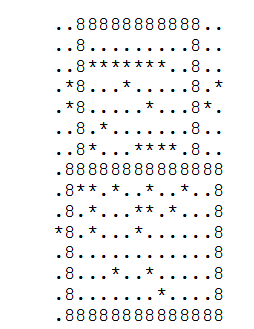
\includegraphics{eight.png}

其中*代表障碍点。
\subsubsection{数据范围}
$n \le 300$
\subsubsection{题解}
应该算是比较简单的题目了。

如果我们能求出$up[i][j][k]$和$down[i][j][k]$分别表示以$(i,j)\rightarrow(i,k)$为上面矩形的底边时上面矩形顶边能有多上面为下面矩形的顶边时下面矩形底边能有多下面,那么最后只要枚举上面矩形的底边,用二维前缀最大值可以$O(1)$算出下面矩形的最大可能值从而算出来。

如何预处理呢?由于$down$与$up$几乎没有区别,我们以$up$为例。

预处理$right[i][j]$表示$(i,j)$向右边最多能走到哪里,求$up[i][j][k]$的时候,假设答案是$x$,那么就要满足$right[x][j] \ge k$,并且$(x,j) \rightarrow (i,j)$与$(x,k) \rightarrow (i,k)$这两条线段上都是没有障碍点的。这个是很容易做的,只要我们先枚举$j,k$,再枚举$i$,沿途开变量记录就行了。

如此一来问题就解决了。
\subsubsection{时空复杂度}
时间复杂度:$O(n^3)$

空间复杂度:$O(n^3)$
\subsection{Codeforces 273D Dima and Figure}
\subsubsection{题意}
给定$n,m$,表示一个有$n \times m$个格子的矩形,要你把一些格子染黑。

限制条件有:
\begin{enumerate}
\item 至少染黑一个点
\item 所有的涂黑的格子形成一个连通块,换句话说,你可以从任意一个涂黑的格子移动到另一个任意涂黑的格子(一个\textbf{黑}格子可以移动到四联通的\textbf{黑}格子里)。
\item 要求任意一个黑点移动到任意一个黑点的最短距离是他们的曼哈顿距离。
\end{enumerate}

\subsubsection{数据范围}
$n,m \le 150$
\subsubsection{题解}
很容易知道,满足题意的,是一个凸多边形。

对于凸多边形来$dp$,是一种非常基本的题型。

凸多边形要求的是,左边界先单调递减,再单调递增,右边界先单调递增,再单调递减。

如此一来,我们就能设$dp[i][l][r][0/1][0/1]$表示到了第$i$行,左边界是$l$,右边界是$r$,左边界应该是单调递减还是单调递增,右边界应该是单调递增还是单调递减。

如此一来能设计出$o(n^5)$的暴力$dp$方程。由于是求和,我们能用二维前缀和优化,所以就没了。
\subsubsection{时空复杂度}
时间复杂度:$O(n^3)$

空间复杂度:$O(n^3)$
\subsection{Codeforces 241F Race}
非常不好描述的题意……

给你一个$n \times m$的网格图,有一些点代表能走过去的街道(并给出了走过他的时间),还有一些路口。

题目会给你一个顺序表,要求按这个顺序依次访问表上的路口。

求第$k$分钟后的位置。

为了保证答案唯一,每个街道要么只能从左往右走,要么只能从右往左走,左右的街道不会和上下的街道相邻。
\subsubsection{数据范围}
$n,m \le 100$

$k \le 100000$
\subsubsection{题解}
应该说是普及组难度的模拟题。

估计是因为题意和题目出处之类的问题没什么人做才不小心被选进集训队作业吧。

说白了就是模拟,没什么好说的。
\subsubsection{时空复杂度}
时间复杂度:$O(nk)$

空间复杂度:$O(nm)$
\subsection{Codeforces 311E Biologist}
\subsubsection{题意}
某人有$n$条狗,他能改变每条狗的性别,改变第$i$条狗的性别要$v_i$的代价。

有$m$个人和他打赌,如果他赢了会得到$w_i$的钱。第$i$富人会给定$k_i$的条件,每个条件都要求\textbf{某些狗}是\textbf{某个}性别,全部满足的话就算你赢。

有一些富人是他的朋友,如果他不能让他的朋友高兴,他还会给朋友$g$的钱作为补偿;但如果不是朋友就不会给钱了。

输出最大收益(可能是负数)。
\subsubsection{数据范围}
$n \le 10^4,m \le 2000$

$k_i \le 10$
\subsubsection{题解}
最小割。

转化为最小损耗。

对狗和人建$n+m$个点。

$S$集代表雄,$T$集代表雌。

这样的话,根据最小割的定义来搞就好了。

我们让要求是$S$集的集合向所有对应狗连无穷大边。

让要求是$T$集的集合让所有狗向他连无穷大边。

然后分别让$S$向他和他向$T$连对应容量边权就行了。
\subsubsection{时空复杂度}
时间复杂度:$O(maxflow(n+m,n+\sum k_i))$

空间复杂度:$O(n+\sum k_i+m)$
\subsection{Google Code Jam World Final 2013 D Can't stop}
\subsubsection{题意}
有$n$个大小为$D$的数集,要求你选择不超过$C$个数和一个区间,使得区间内的每个数集都包含$C$个数中的某一个数,最大化区间长度。

$T$组数据。
\subsubsection{数据范围}
$n \le 10^5$

$D \le 4,C \le 3,T \le 10$
\subsubsection{题解}
称第$i$个数集第$j$个数为$v[i][j]$。

利用$D$和$k$都很小的特点,从低维逐步向高维扩展。

首先,设$go1[i][j]$为区间左端点在$i$,选择了第$j$个数,最远能延伸多远。

显然,如果数集$i+1$不包含这个元素,就是$i$,否则能拿$go1[i+1]$递推过来。就能解决$C=1$了。

假设$C=2$,第一个数是第$i$个数集的第$j$个,我们很容易发现一个贪心性质:第二个被选的数一定属于数集$go1[i][j]+1$,假设是第$k$个,那么设$go2[i][j][k]$为这种情况下能延伸多远。

这个怎么算呢?先设$x=go1[go1[i][j]+1][k]$,那么如果数集$x+1$不包含元素$v[i][j]$,就是$x$,否则可以由$go2[go1[i][j]+1][k]$递推过来。$C=2$就解决了。

那么$C=3$怎么做呢?如法炮制,是可以递推的。
\subsubsection{时空复杂度}
时间复杂度:$O(TnD^{C+1})$
\subsection{Google Code Jam World Final 2008 E The Year of Code Jam}
\subsubsection{题意}
有一张$n$行$m$列的网格,有一些强制要求填$0$,有一些强制要求填$1$,有一些要你填$0$或$1$。

如果你在某个位置填了一个$1$,你就能得到$4-$相邻的格子上的权值。

相邻是指的四联通。

求最大收益,$T$组数据。
\subsubsection{数据范围}
$n,m \le 50$

$T \le 100$
\subsubsection{题解}
又是一道赤裸裸的最小割。

不明白为什么GCJ别的题那么神,最小割题却这么裸。

把格子进行黑白染色。

最大化收益改为最小化损耗。

对于黑格子,我们让$S$向他连他不填$1$的损耗。

对于白格子,我们让他向$T$连他不填$1$的损耗。

对于相邻的两个格子,我们让黑格子向白格子连一条权值为$2$的边。
\subsubsection{时空复杂度}
时间复杂度:$O(Tmaxflow(nm,nm))$

空间复杂度:$O(nm)$
\subsection{Codeforces 251D Two Sets}
\subsubsection{题意}
给你一个$n$个数的集合$a$,要你把他分成两个集合$A$与$B$。

首先要最大化$A$集合所有元素异或和+$B$集合所有元素异或和。

在满足条件的情况下,还要最小化$A$集合所有元素异或和。
\subsubsection{数据范围}
$n \le 10^5$

$0 \le a_i \le 10^{18}$
\subsubsection{题解}
先看第一问。

用高斯消元法,能解决这么一个问题:要求选出一个子集,满足异或和的某一位是某个值,并求出一组解。

有了这个武器,我们就能进行一个判定。

对于每一位,如果所有元素的异或和这一位是$1$,那么无论怎么分,一定是某一边这里是$1$,另一边这里是$0$。所以对第一问是无影响的。

不过如果这一位是$0$的话,$A,B$集合的异或和的这一位就有两种可能:$(1,1),(0,0)$。显然,我们需要贪心的让他们尽可能变成$(1,1)$。

要做的就是判断能不能是$(1,1)$,高斯消元。

如此就能保证第一问了,然后是第二问,显然的,我们要在满足第一问的情况下,尽可能的让某些位的$A$集合的异或和是$0$,继续用高斯消元。
\subsubsection{时空复杂度}
时间复杂度:$O(n \log^2 n)$

空间复杂度:$O(n)$
\subsection{Codeforces 274E Mirror Room}
\subsubsection{题意}
给你一个$n \times m$的网格,有$k$个障碍点,一个点光源。

点光源能向东北、东南、西北、西南中的某个方向射出一条光线。

光线撞到障碍或边界会反射,几种情况如下:

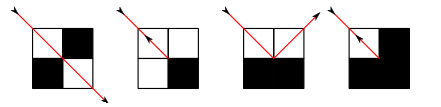
\includegraphics{mirror.png}

显然会出现循环。要你统计至少被穿过一次的方格的个数。

被穿过当且仅当方格中心被穿过。
\subsubsection{数据范围}
$n,m,k \le 10^5$
\subsubsection{题解}
问题分两步:模拟与统计。

先看模拟部分。主对角线方向的$x-y$是不变的,副对角线方向的$x+y$是不变的。

对每条对角线按顺序存这条线上的障碍点,模拟的时候就在对应对角线上二分下一个,然后在这条对角线上插入一个区间即可。

至于统计,我们可以对于每条对角线,求对应的区间并。

但是这就有个问题,如果主对角线和副对角线有交点,会重复计算。

一般来说,处理方法应该是用扫描线加树状数组计算交点个数,但这题有个很好的性质:不会有交点!

证明很简单,主对角线变成副对角线(或者反过来)只有图三那种情况,我们可以发现,这种情况的$x+y$的奇偶性一定会变化!

所以主对角线经过的点与副对角线经过的点是不会有交点的,大大简化了代码量。
\subsubsection{时空复杂度}
时间复杂度:$O(n \log n)$

空间复杂度:$O(n)$
\subsection{USACO February Contest 2014, Airplane Boarding}
\subsubsection{题意}
数轴上$n$头奶牛按顺序排在$[-n+1,0]$处,其中站在$0$的是第$n$号奶牛。

有一个排列$S_1,S_2,\cdots,S_n$,表示的是每头奶牛的目的地。

奶牛群会每秒向前走一步,如果第$i$只奶牛走到了自己的目的地$S_i$,他就会在这里停住$T_i$秒,他后面的那头奶牛(如果有的话)也不能往前走了,如果他后面的后面的奶牛(如果有的话)也不能往前走了,以此类推。

$T_i$秒之后,奶牛坐了下来,不会挡住后面的奶牛了。

求要多少时间让所有奶牛都坐下来。
\subsubsection{数据范围}
$n \le 2\times 10^5$
\subsubsection{题解}
我们定义一个二元组$(x,T)$表示在时间$T$不能跨越点$x$。

维护一个这样的二元组集合,刚开始有一个$(0,0)$。

倒着考虑,先考虑$[i+1,n]$的奶牛,再考虑第$i$个奶牛,第$i$个奶牛坐下的时间,应该是在二元组里所有满足$x<S_i$的二元组里,找一个$T-x+S_i+T_i$最大的,令其为$V$,也就是维护$T-x$的最值。

之后,我们要插入一个二元组$(S_i,V)$。同时,要把所有第一维小于$S_i$的二元组$(x,T)$改写成$(x-1,T)$。

我们可以用平衡树来维护这个二元组。
\subsubsection{时空复杂度}
时间复杂度:$O(n \log n)$

空间复杂度:$O(n)$
\subsection{USACO Open Contest 2010, Triangle Counting}
\subsubsection{题意}
给你平面上$n$个点,要你选$3$个点,不包含原点,求方案数。
\subsubsection{数据范围}
$n \le 10^5$
\subsubsection{题解}
直接做会略显麻烦,正难则反,计算有多少不包含原点。

将所有点按极角排序后,枚举极角最小的那个点,显然会存在一段区间,使得区间内$[l,r]$任意两个点与他组合成的三角形都不包含原点,贡献是${{r-l+1} \choose 2}$。

拿${n \choose 3}$减去这些贡献就行了。
\subsubsection{时空复杂度}
时间复杂度:$O(n \log n)$

空间复杂度:$O(n)$
\subsection{Codeforces 332D Theft of Blueprints}
\subsubsection{题意}
给出一个n个点的带权无向图,有若干条边,每条边为点$i$向点$j$连一条权值为$c_{i,j}$的边。

保证对于任意一个大小为$k$的顶点集合$S$,恰有一个点与$S$的每个点都有边,令这个点为$v(S)$,对$S$操作的代价是$S$的每个点到$v(S)$的边权之和。求操作一个大小为$k$的集合的期望边权。
\subsubsection{数据范围}
$n \le 2 \times 10^3$
\subsubsection{题解}
对于一个点$i$,假设他连出去了$x$个点,那么对于这${x \choose k}$个子集,都会是以$i$为$v(S)$的。

对于一条存在的边$i,j$,$i$连出去了$x$个点,他会出现在${{x-1} \choose {k-1}}$个集合中,所以会对总权值造成这么多的贡献。

预处理一些东西之后就能这么计算答案了。
\subsubsection{时空复杂度}
时间复杂度:$O(n^2)$

空间复杂度:$O(n^2)$
\subsection{Google Code Jam World Final 2014 F ARAM*}
\subsubsection{题意}
你在玩一款游戏,每次会随机成为一个角色。有$n$种角色,你选择第$i$个角色有$p_i$的概率赢。

如果你有至少1游戏币,你可以选择“Reroll”,“Reroll”会消耗1游戏币,之后又随机成为一个角色。

你刚开始有R个游戏币。每玩一盘游戏,你会得到$\frac{1}{G}$的游戏币。你所拥有的游戏币将以$R$为上限。

你会进行$10^{100}$次游戏,要你制定最优策略,求在此情况下期望的获胜比例。

T组数据。
\subsubsection{数据范围}
\begin{enumerate}
\item 对于测试点$1 \sim 2$,有$T=100,n,R,G \le 10$
\item 对于测试点$3 \sim 5$,有$T=1,n \le 200,R,G \le 3$
\item 对于测试点$6 \sim 8$,有$T=10,n \le 200,R,G \le 3$
\item 对于测试点$9 \sim 10$,有$T=1,n \le 1000,R,G \le 3$
\item 对于测试点$11 \sim 14$,有$T=10,n \le 500,R,G \le 20$
\item 对于测试点$15 \sim 20$,有$T=1,n \le 1000,R,G \le 20$
\end{enumerate}
\subsubsection{题解}
题目要求的是平均数,平均数一般直接做不好做。

我们有一个通用办法,叫做分数规划。即二分答案,假设答案是$\frac{x}{y}$,我二分的答案是$p$,若$x-py>0$,则$p<\frac{x}{y}$。如此可以解决一般的和平均数有关的题。

题目说游戏进行$10^{100}$次,由于数目非常大,我们可以想象这个次数远远超过函数收敛下来使得我们的精度足够的次数。我们不妨假设题目是进行无限轮次。

还有就是所谓的最优策略。我们可以想象,假设在钱数一样的时候,抽到$i$我``Reroll'',抽到$j$我不``Reroll'',可是$p_j<p_i$,这显然不是优秀的策略。于是我们知道,假设钱数一定,一定是最弱的几个会``Reroll'',其余的则不会。

假设二分的答案为$Q$,我们需要定义一个量$s$,表示的是:赢一盘+1,玩一盘-Q,最终的期望值。

以上就是我们需要用到的前提。

设$A_i$表示钱数为$i$时,要得到$i+\frac{1}{G}$的钱,过程中的$s$。

而如果$i=R$,状态的定义要改变,为再一次变回$R$过程中的期望的$s$。

若$i<1$,则无法``Reroll'',于是
	
\[A_i=\frac{1}{n}\sum_{j=1}^n (P_j-Q)\]

若$1 \le i < R$,我们将角色按$p$值排序,枚举一个$k$表示最弱的$k$个要``Reroll''
	
\[A_i=\frac{k}{n}\sum_{j=0}^G A_{i-1+j/G}+\frac{1}{n}\sum_{j=k+1}^n(p_j-Q)\]

移项可得$A_i$的表达式。

类似的,若$i=R$,则

\[A_i=\frac{k}{n}\sum_{j=0}^{G-1} A_{i-1+j/G}+\frac{1}{n}\sum_{j=k+1}^n(p_j-Q)\]

事实上,$A_R$即为所求。

为什么?

不妨设$\forall i<R$,均有$A_i<0$,因为我们知道$A$单调不减,如果存在$A_i \ge 0 ,i<R$,我们不如让$R$变成$i$。

我们把$10^{100}$次操作这么分开看……许许多多次的从$R$变到$R$,最后可能变成某个值。

而我们要算的是$s$不是比例,$s$可加可减给我们带来了极大地便利。

容易知道,$A_i \ge -1$,所以最后一段的$s$的期望值是不超过$-RG$的。

前面的话,如果有$T$次$R$变到$R$,我们可以看作$A_RT$,这是个庞大的天文数字。一个是大约$A_RT$的数,一个是大于$RG$的数,要判断的是他们的和是否大于0,我们自然可以无视掉后面的数了。

换句话说,如果我们把$10^{100}$理解为正无穷,我们根本不必在意最后的那么一小段,而是完全可以理解为$R$到$R$到$R$无限循环下去。

于是只要拿$A_R$与$0$作比较即可。
\subsubsection{时间复杂度}
时间复杂度$O(TnRG)$。
\subsection{Codeforces 305D Olya and Graph}
\subsubsection{题意}
称这样的有向图为good图:

\begin{enumerate}
\item 从点$i$出发,可以到达点$i+1,i+2,\ldots,n$。
\item 任意从$u$到$v$的有向边满足不等式:$u<v$。
\item 两点之间最多有一条边。
\item 对于一对点$i,j(i<j)$,若$j-i \le k$,那么从$i$到$j$的最短距离等于$j-i$。
\item 对于一对点$i,j(i<j)$,若$j-i>k$,那么从$i$到$j$的最短距离等于$j-i$或$j-i-k$。
\end{enumerate}

给定图的一部分,要求有多少个不同的图是good的。
\subsubsection{数据范围}
$n \le 10^6$
\subsubsection{题解}
点$i$必须向$i+1$连边,可以向$i+k+1$连边。

不能存在点$i \rightarrow i+k+1,j \rightarrow j+k+1,i+k+1 \le j$的局面。

到了这一步问题就差不多结束了。对于每个区间$[i,i+k+1]$,如果可以以$i$为最小的连向$i+k+1$的点,那么区间里任意一个没有被输入的点都要么选要么不选。会带来$2$的若干次方的贡献。
\subsubsection{时空复杂度}
时间复杂度:$O(n)$

空间复杂度:$O(n)$
\subsection{Codeforces 348E Pilgrims}
\subsubsection{题意}
有一棵黑白树,你可以摧毁一个白点,一个黑点不高兴当且仅当他不能到达任何在原树中离他最远的黑点。要你最大化不高兴的黑点数目以及求出方案数。
\subsubsection{数据范围}
$n \le 10^5$
\subsubsection{题解}
为了方便描述,我们先忽视所有有关黑白色的问题。

由于涉及到最远点的问题,我们引入一些中心的概念。

树中最长的路径称为树的直径。对于给定的树$T$,直径不一定唯一。但可以证明各直径的中点唯一(不一定恰好是某个结点,可能在某条边的内部),我们称之为{\textbf{中心}}。

我们还能证明,任何点走到离他的最远点一定经过了中心。如果中心不是某个节点而在边的内部,可以想象既然经过了这个点,必然经过边上的两个点。

我在此定义概念{\textbf{类中心}}。大概就是说,如果中心恰好是节点,那么他也就是类中心,否则就是它所在的边的任意一个端点。(这只是我在这道题上的定义,并非学术用语)

可以证明,任何点走到离他的最远点一定经过了类中心。

既然类中心有这样优美的性质,那么它是否对我们解题有帮助呢?

我们将无根树变有根树,找到一个类中心,将它提根。

类中心的找法很容易,只需任意求出一条直径,根据定义来找即可。直径可以用做两次最远点或者树形动态规划的方法在$O(n)$时间内求出来,具体算法是noip级别知识,不再赘述。

我们枚举每个点,我们要做的就是看有哪些黑点走到最远点必须经过他。

利用类中心的性质,我们知道任意$a$走到$a$的最远点时必须经过根。判定$a$走到$a$的最远点是否必须经过$b$分两种情况:

\begin{enumerate}
\item $a$不在$b$子树内。我们只需记录每个子树内最深点的深度,拿$a$所在子树的深度是不是所有子树中最深、次深之类的情况出来讨论即可。
\item $a$在$b$子树内。$a$走到$a$的最远点,必须经过根,于是必须经过$b$了。
\end{enumerate}

当然我们还要注意到题目要求的不是单纯意义上的最远点,而是黑点之间的。

我们只需稍微改变一下定义即可。我们把直径理解为黑点之间的最长路,中心、类中心的定义跟着变化;要维护的东西(如每个子树内最深点的深度)也跟着把``点''变成``黑点''即可。
\subsubsection{时空复杂度}
时间复杂度:$O(n)$

空间复杂度:$O(n)$
\subsection{Google Code Jam World Final 2013 C X Marks the Spot*}
\subsubsection{题意}
平面上有$4n$个点,\textbf{保证无三点共线},要你画一个形如X的形状,即两条互相垂直的直线。

要求两条直线上没有点。他们将平面分成了$4$份,每一份都会有恰好$n$个点。
\subsubsection{数据范围}
$n \le 2500$
\subsubsection{题解}
假如我们来已知第一条直线的倾斜角,那么由于这条直线的两侧恰好有$n$个点,我们便可以算出中心的横坐标:就是将坐标轴旋转后的点的中位数在转回来!

同理,我们也知道纵坐标。换句话说,一旦倾斜角定了,我们就能确定一个中心。

设新坐标轴的第一象限有$f(\alpha)$个点,显然另外三个象限点数是知道的。我们要解方程$f(\alpha)=n$。

若$\alpha$取到某个值时,直线上有点,那么将他偏移无限小量后,前后的函数值相差不会超过$1$(可以用两侧点数都是$2n$来想)。那么我们证明了函数值在整数上是连续的。

$f(\frac{\pi}{2})=2n-f(0)$,若$f(0)=n$则找到了一组解,否则必然一个小于$n$一个大于$n$,而函数连续,可以用二分法求解。

复杂度可以做到$O(n \log n)$,但由于我偷懒求中位数时用了排序,所以我的复杂度多了一个$\log$。
\subsubsection{时空复杂度}
时间复杂度:$O(n \log^2 n)$

空间复杂度:$O(n)$
\newpage
\section{试题泛做10}
\subsection{Google Code Jam World Final 2012 D Twirling Towards Freedom*}
\subsubsection{题意}
给你平面上$n$个点,刚开始你在原点,你能进行最多$m$次操作,每次对一个给定的点进行的操作是绕这个点顺时针旋转$90^{\circ}$。

求你离原点最远能有多远。

$T$组数据。
\subsubsection{数据范围}
$T \le 100,n \le 5000$
\subsubsection{题解}
一个点绕某个点旋转$4$次会回来,所以我们可以看做进行$[m-3,m]$次操作,这样就把“最多”变成“恰好”了。

如果我们用复数$a+bi$来表示一个点$(a,b)$的话,那么绕原点顺时针旋转$90^{\circ}$可以看做是乘以$-i$。

假设$P$绕着$Q$旋转至$P_1$的话,我们很容易推出$P_1=Q+(P-Q)\cdot (-i)=-i\cdot P+(i+1)\cdot Q$。

如果继续沿着这个思路来推下去的话,我们会发现一个结论是说:假设进行$m$操作分别是对$Q_1,Q_2,Q_3,Q_4,\cdots,Q_m$,那么能写成$a_0 \cdot P+\sum\limits_{k=1}^m a_i \cdot Q_i$的形式。

$P$是$(0,0)$,可以忽略。其中$a_i$是一个复数,表示的是对应的系数,他只可能是$1+i,1-i,-1+i,-1-i$。推前几个能够知道,$a_i=a_{i+4}$。

有了这个之后,我们就能把他写成$a_1(Q_1+Q_5+Q_9\cdots)+a_2(Q_2+Q_6+Q_{10}\cdots)+a_3(Q_3+Q_7+Q_{11}\cdots)+a_4(Q_4+Q_8+Q_{12})$。

一个显然的结论是,最优解$Q_i=Q_{i+4}$,这个能用向量的方法证明。

这样一来的话,假设输入的第$i$个点是$p_i$,我们就会有$4$个向量集,要在$A,B,C,D$个选一个,然后加起来,然后得到的向量的模最大。

很显然得到的会在凸包上,我们把四个向量集求凸包,把四个凸包给合并,这是经典的闵可夫斯基和问题。
\subsubsection{时空复杂度}
时间复杂度:$O(Tn \log n)$

空间复杂度:$O(n)$
\subsection{USACO March Contest 2010, StarCowraft}
\subsubsection{题意}
现有$n$个约束条件,形如$ax+by+cz<0$或者$ax+by+cz>0$。

此外还要求,$x,y,z$均为正实数,且两两之间比值不会超过$100$。

有$m$组询问,询问是否存在$ax+by+cz<0$、$ax+by+cz=0$、$ax+by+cz>0$。
\subsubsection{数据范围}
$n \le 300$

$m \le 2000$
\subsubsection{题解}
虽然看起来是个半空间交,但很容易想到(题意也提醒了我们)只要考虑比值即可。

如此一来就转化为了半平面交。

求出半平面交后对于每组询问在半平面交上搞搞就行了,我就是直接枚举半平面交上的所有顶点。不过这里有很多细节要注意,虽然都是小细节。

由于数据范围很小,半平面交可以用切割法求。
\subsubsection{时空复杂度}
时间复杂度:$O(n^2+nm)$

空间复杂度:$O(n)$
\subsection{Codeforces 343E Pumping Stations}
\subsubsection{题意}
有一张$n$个点$m$条边的带权无向图。

要你构造个排列$a$,排列的收益是$\sum_{i=2}^n mincut(a_{i-1},a_i)$。

$mincut(S,T)$代表要你求图中以$S,T$做源点、汇点的最小割大小。

最大化收益值。
\subsubsection{数据范围}
$n \le 200$

$m \le 1000$
\subsubsection{题解}
首先,我们要知道一种叫做“最小割树”的东西,在此不再赘述。

知道了这个,我们可以通过做$n$次最小割就求出任意两点间的最小割,并且知道两点间的最小割值等于路径上的边权最小值。

如此一来,构造出树(其实不用显式构造)后就能贪心了。贪心过程是这样的。

每次找到最小边,然后删去之后形成两个连通块,在两个连通块分别递归。
\subsubsection{时空复杂度}
时间复杂度:$O(n\times maxflow(n,m)+n^3)$

空间复杂度:$O(n^2)$
\subsection{Codeforces 286E Ladies' Shop}
\subsubsection{题意}
现有一个大小为$n$的正整数数列$a$,有值域上限$m$即保证$1 \le a_i \le m$。

要你构造一个单调递增的不超过$m$的正整数数列$b$,满足
\begin{enumerate}
\item 对于任意$a_i$,均存在$b$的一个子集和等于$a_i$。
\item 对于$b$的任意一个子集和,只要不超过$m$,就要求这个值在数列$a$中出现过。
\item 要求最小化$b$的元素个数。
\end{enumerate}

输出任意一组解或输出无解。
\subsubsection{数据范围}
$n,m \le 10^6$
\subsubsection{题解}
贪心的观察一些特殊情形,我们会发现原问题等价于找所有$a_i+a_j=a_k$无解的$a_k$!

由于是3-sum问题,所以不能从正常方面突破,注意到值域有限且是正整数,我们可以用快速傅里叶变换来解决这个问题!

即我们记$c[i]$为$i$这个数有没有在原数列过,如此一来,我们考虑计算$cnt[i]=\sum c[j]*c[i-j]$,只要计算出$cnt$就能解决这个特殊的3-sum问题了。

而$cnt[i]=\sum c[j]*c[i-j]$,这又是一个标准的卷积形式,我们自然能用FFT解决。
\subsubsection{时空复杂度}
时间复杂度:$O(n \log n)$

时间复杂度:$O(n)$
\subsection{Codeforces 341E Candies Game*}
\subsubsection{题意}
有$n$个数$a_1,a_2,\ldots,a_n$,你每次能进行如下操作:

\begin{enumerate}
\item 选择$i,j,a_i \le a_j$。
\item 从箱子$j$中拿出$a_i$个糖果放到箱子$i$里。显然若$a_i=a_j$,箱子$j$就空了。
\end{enumerate}

你的任务是问能否在不超过$10^6$步里面变成恰好两个箱子不空的局面,如果能输出任意一组解,否则输出无解。
\subsubsection{数据范围}
$n \le 1000$

$\sum\limits_{i=1}^n a_i \le 10^6$
\subsubsection{题解}
构造题。

假设有$3$个数$a_i \le a_j \le a_k$,如果能在$O(\log a_j)$步里把$a_j$变成$a_j \mod a_i$,那么由于$x \mod y \le \frac{x}{2}$,我们就能在$O(n \log^2 a)$步实现。

令$a_j=k_1a_i+r_1,a_k=k_2a_i+r_2$。

我们知道无论是执行操作$(i,j)$还是执行操作$(i,k)$,都能让$a_i$乘以$2$。(关键在于即使$\lfloor \log k_1 \rfloor$步操作的过程都是$(i,j)$,中途仍然不会出现$a_j < a_i$的情况,所以每次都是$a_i$翻倍)

做$\lfloor \log k_1 \rfloor$步$(i,j)$或者$(i,k)$,$a_1$的变化是$2a_1,4a_1,8a_1,\ldots$。

先把$k_1$的二进制表示写出来,假设$k_1=\sum\limits_{i=1}^m 2^{p_i}$,在做这$\lfloor \log k_1 \rfloor$步操作时,第$x$次操作$a_1$会变成$2^x a_1$,如果$x \in p$,就执行$(i,j)$从而让$a_j-2^x a_i$。

这样就达到了将$a_j$变成$a_j \mod a_i$的效果。于是无解的情况是刚开始就只有不到$2$个数非零,其余都能在规定步数内出解。
\subsubsection{时空复杂度}
时间复杂度:$O(n \log^2 a)$

空间复杂度:$O(n)$
\subsection{Codeforces 346E Doodle Jump*}
\subsubsection{题意}
数轴上有$n$个点,第$x$个点的坐标是$ax \mod p$,其中$(a,p)=1$。

你从原点出发,每次能跳不超过$h$的距离。

问能不能跳到最大的那个点。

$T$组数据。
\subsubsection{数据范围}
$T \le 10^4$

$a,n,p,h \le 10^9$
\subsubsection{题解}
问题的关键在于缩小数据规模转化为一个等价问题。

首先转化为找最长的一段没有点的区间,特判掉$an < p$的情况(即只讨论会覆盖$p,2p,3p,\ldots,\lfloor \frac{p-1}{a} \rfloor p$的情况)

来看一个$a=5,p=23$的例子:

0  5  10  15  20

2  7  12  17  22

4  9  14  19

1  6  11  16  21

3  8  13  18

一旦进入下一轮循环就重新分组。

最长的没有点的区间长度不会超过$a$,不会跨越点$ak,ak<p$。

题解给出了这么一个结论:最长的没有点的区间一定在$[\lfloor \frac{p}{a} -1 \rfloor a,\lfloor \frac{p}{a} \rfloor a)$内部。比如$a=5,p=23$这个例子,无论$n$等于几(前提是$an \ge p$),答案一定在$[15,20)$内。

接下来是证明。像这个例子,显然答案是不会在$[0,15)$内的,因为$[0,15)$里有的点,在$[15,20)$里不一定有对应的;但反之$[15,20)$里任何一个出现了的点,在$[0,5),[5,10),[10,15)$里一定有和他在同一组里的对应点。

我们唯一要考虑的是答案可不可能在$[20,23)$里。事实上这也是不可能的,因为最后一段区间的长度本身就已经小于$a$了,讨论各种情况后是可以证明不会出现剩余的那一段有更长的空白区间的情况的。

如此一来,长度就由$p$变成了$a$,$a$变成了$a- p \mod a$,这样子就已经会让规模变小,按理来说应该是能通过这题的。但有没有更靠谱的时间复杂度的做法呢?

我们发现,$a=1$与$a=p-1$是对称的局面,换句话说,可以用$p \mod a$来代替$a- p \mod a$。我们每次在这两个数中取小的那个,就能让$a$的规模每次减半了。
\subsubsection{时空复杂度}
时间复杂度:$O(T \log a)$

空间复杂度:$O(\log a)$
\subsection{Codeforces 256D Liars and Serge}
\subsubsection{题意}
现在有$n$个人,有人只会说真话,有人只会说假话,你向他们提问:有几个人说真话。

说真话的人一定会告诉你正确答案,说假话的人一定会告诉你一个错误答案。$n$个人的答案会形成一个数列。

看到这个数列后,聪明的你脱口而出:恰好有$k$个人肯定撒谎了。那么求有多少个答案数列会让你这么说。

\textbf{保证$n$素因子只有$2$。}
\subsubsection{数据范围}
$1 \le k \le n \le 256$
\subsubsection{题解}
令$b_i$为$a_j=i$的$j$的个数。

问题转化为要求恰好$k$个$i$使得$b_{a_i} \neq a_i$。

考虑动态规划。

$dp[i][j][k]$表示考虑到了第$i$个数,当前有$j$人,有$k$个人一定说谎。

枚举有$x$个人写了$i$,如果$x=i$代表从$dp[i-1][j-x][k]$转移,否则从$dp[i-1][j-x][k-x]$转移,转移的时候呈乘上组合数。

说白了就是个完全背包的问题,所以空间能降为$O(n^2)$。

但这样子时间是$O(n^4)$的,卡卡常数能通过$n \le 128$,但$n=256$怎么办呢?

注意到题目还有一句话:$n$是$2$的整数次幂。

如果我们能过$n=128$的点,那还有什么点不能过呢?不会有$n=129,n=130,\ldots$,只会有$n=256$的点。而$n=256$的点又只有$k=1,\ldots,256$这么多个。

是的!最终做法是——打表!(妈呀我已经不知道该怎么评论这种题目了)
\subsubsection{时空复杂度}
时间复杂度:对$n\le 128$是$O(n^4)$,对$n=256$是$O(1)$

空间复杂度:$O(n^2)$
\subsection{Codeforces 325E The Red Button}
\subsubsection{题意}
给定$n$,要你构造一个$0 \sim n-1$的排列$a$,满足在模$n$意义下,$a_i$要么等于$2a_{i-1}$要么等于$2a_{i-1}+1$。并且还要满足$2a_{n-1}=0$或者$2a_{n-1}+1=0$。
\subsubsection{数据范围}
$n \le 100000$
\subsubsection{题解}
听说正解是用欧拉回路什么的做的。

我的做法我也不是很会证明正确性(或者说完全觉得不对)。奇数无解,倒着考虑,令$a_n=0$,然后假设得到了$a_i$,若$\lfloor \frac{a_i+n}{2} \rfloor$没出现过就填到$a_{i-1}$,否则把$\lfloor \frac{a_i}{2} \rfloor$填入$a_{i-1}$,似乎偶数一定能出解的样子……
\subsubsection{时空复杂度}
时间复杂度:$O(n)$

空间复杂度:$O(n)$
\subsection{Codeforces 309E Fence}
\subsubsection{题意}
有$n$个区间$[l_i,r_i]$,要你求一个排列,使得所有相交的区间在排列中的位置的距离差的最大值最小。
\subsubsection{数据范围}
$n \le 1000$
\subsubsection{题解}
感觉是神题……有点似懂非懂。

由于是最大值最小,所以很容易想到二分答案。

于是要做的是判断能否安排一个顺序,相交的区间的位置差不能超过定值$D$。

先把区间按照右端点排序。

依次考虑第$i$个区间放谁,此刻有个$limit$数组,表示每个区间的能放得位置的最大值。

可以理解为找区间和位置的一个一一对应关系,然后每个区间都有$limit$数组作为约束条件。

根据Hall定理,为了保证能由完备匹配,如果有$i$个数要放在前$i$个位置,就应该在这$i$个数里找一个右端点最小的区间。
\subsubsection{时空复杂度}
时间复杂度:$O(n^2 \log n)$

空间复杂度:$O(n^2)$
\subsection{USACO December Contest 2008,Fence}
\subsubsection{题意}
平面上有$n$个点,要你选一些点画出一个凸多边形,最大化选出的点的个数。
\subsubsection{数据范围}
$n \le 250$
\subsubsection{题解}
一个凸多边形,一定可以找到一个点为起点,顺次遍历凸多边形,遍历过程中走过的$n$个向量极角是单调递增的。

有了这个性质,我们就能$dp$了。

首先,我们枚举这个点,然后就是要找一个向量序列,单调递增,并且向量两两相接,开头结尾都是这个点。

设$dp[i][j]$表示最后一条边是$(i,j)$的最多点数。

依次枚举所有向量,假设枚举到向量$\overrightarrow{ij}$,我们就拿$max(dp[k][i]+1)$来更新$dp[i][j]$,要求$\overrightarrow{ki}$的极角小于$\overrightarrow{ij}$。

当然优化下来是很简单的,我们只要一开始就把向量排序,按极角大小依次枚举过去,就不用考虑$\overrightarrow{ki}$极角小于$\overrightarrow{ij}$的问题了,同时维护一个$g[i]$表示以$i$为结尾的最大值,就能写成$g[i]+1$了。
\subsubsection{时空复杂度}
时间复杂度:$O(n^3)$

空间复杂度:$O(n^2)$
\subsection{Codeforces 241E Flights}
\subsubsection{题意}
现有一个有向无环图,每条边的边权都是$1$。

要求你把某些边的边权改成$2$,使得任何一条$1$到$n$的路径的长度相等。判断有无解,有解输出任意一组合法解。
\subsubsection{数据范围}
$n \le 1000,m \le 5000$
\subsubsection{题解}
我们只用关心$1$能到并且能到$n$的点。可以删去除此之外的所有点。

一个显然的性质新图的任何一个点$i$,都有$1$到$i$的任意路径长度相等,我们可以设这个长度为$x_i$。

对于边$u \rightarrow v$,有约束条件$1 \le x_v-x_u \le 2$。

同时要求所有$x_i$都是整数。$x_1=0$。

直接上差分约束系统就行了,差分约束系统算出来的一定都是整数,并能解决以上所有约束。
\subsubsection{时空复杂度}
时间复杂度:$O(SPFA(n,m))$

空间复杂度:$O(n+m)$
\subsection{Google Code Jam World Final 2013 A Graduation Requirements}
\subsubsection{题意}
有一个长度为$n$的环形跑道,某些时刻$t_i$会有一辆车从点$a_i$逆时针以$1$路口每秒速度走向$b_i$。保证$0 \le t_i \le m$,$m$给定。

你要选择一个时刻和一个地点,要求从这个时刻这个地点开一辆车顺时针以$1$路口速度每秒行走,能滑行一段最长的时间,要求这段时间不能与任何一辆车相交,并且在$[0,m]$。

求最长时间。

$T$组数据。
\subsubsection{数据范围}
$T \le 10,n \le 1000$
\subsubsection{题解}
如果用一个点来描述一个事件的话,会有三维,不方便处理。

我们可以不用一个点来描述而用一个线段描述,从而减少一维。假设$(x,y)$表示时间$t$时在点$y$,那么其他人的车的行走路线会是若干条斜率为$1$的线段(如果越界了就把越界部分平移回来,看成两条线段),而你的行走路线是若干条斜率为$-1$的线段),线段都要求在整点上。

给你一些斜率为$1$的线段,你需要画一条斜率为$-1$的线段,使得与其他线段严格不相交,最大化线段长度。

如果离别的线段很远,能通过平移的方法进行调整,使得有一个最优解,他存在一个点,平移一步就会跟别的线段的某个端点相交。

这样的话,我们枚举所有线段端点的周围,计算向前向后能延伸多长,加起来就行了。

由于是环形,所以不是特别好处理,但这只是细节问题。
\subsubsection{时空复杂度}
时间复杂度:$O(Tn^2)$

空间复杂度:$O(n)$
\subsection{Google Code Jam World Final 2011 A Runs}
\subsubsection{题意}
给定一个只由小写字母组成的字符串$S$。

称一个字符串的$run$数为极大的各个字符都相同的子串个数。

问有多少种将这个字符串重排的方案数,$run$值与这个字符串相同。

两个方案数不同当且仅当重排后的字符串不同。
\subsubsection{数据范围}
$|S| \le 450000$

$run$的个数不超过$100$
\subsubsection{题解}
设$run$数为$m$。

由于字符串很长,但字符集只有$26$个,考虑按字符集来$dp$。

设$dp[i][j]$表示前$i$种字母,有$j$个$run$。

转移的时候,如果字符串里第$i$号字母,并有$s$个,我们考虑插空,即将$s$个字母$i$分成若干段插入进去,插入进去之后这些段互不相邻。

插入的时候,分两种情况,一种是插在之前的完整段中间,比如把插$b$入$aa$中间形成$aba$。另一种是不插在其他字符中间,比如把$c$插在$aabb$中形成$aacbb$。

我们强行爆枚有几个第一种情况以及有几个第二种情况,假设$x$个第一种情况,$y$个第二种情况。第一种情况会让$run$数加$2$,第二种会让$run$数加$1$。

前$i-1$种字母的$run$数应该是$j-2x-y$,假设前$i-1$种字母共$cnt$个,就有$cnt-(j-2x-y)$个位置来插入第一种情况,有$j-2x-y+1$个位置插入第二种情况,用组合数算一下就好了。以及我们还要算把一个长度为$s$的字符串分割成$x+y$个字符串的方案数,这个也是用组合数算一下就好了。

计算完这些后,就能$dp$了。
\subsubsection{时空复杂度}
时间复杂度:$O(26m^3)$

空间复杂度:$O(|S|+26m)$
\subsection{USACO March Contest 2009, Cleaning Up}
\subsubsection{题意}
有$n$个数,每个数都不超过$m$。

要你分成若干段,每一段的权值是这一段的数字种数的平方,要你最小化所有段的权值和。
\subsubsection{数据范围}
$n,m \le 10^5$
\subsubsection{题解}
暴力的$dp$方程是很显然的,$dp[i]$表示$1 \sim i$的答案,$dp[i]=min(dp[j]+score(j+1,i))$,$score(l,r)$表示计算区间$[l,r]$的权值。

考虑优化,注意到我们可以一个数字一组,这样子答案恰好是$n$,所以要求$dp[i] \le n$,对于$i$的决策点$j$,就要求区间$[j,i]$的不同数的个数不能超过$\sqrt{n}$。

如此一来,用个大小为$\sqrt{n}$的队列存最后的$\sqrt{n}$种数暴力转移就行了,应该算是个水题。
\subsubsection{时空复杂度}
时间复杂度:$O(n\sqrt{n})$

空间复杂度:$O(n)$
\subsection{Codeforces 316D PE lesson}
\subsubsection{题意}
现有$n$个人,第$i$个人手上有一个编号为$i$的球。

现在能进行一些交换,每个交换操作是把第$i$个人和第$j$个人手上的球进行交换。

每个位置上有个交换次数上界$b_i$,指的是这个人能参与交换的次数,$b_i$不会超过$2$。

求最终有多少种不同的局面,两个局面不同当且仅当某个人手上的球的编号不同。
\subsubsection{数据范围}
$n \le 10^6$

$1 \le b_i \le 2$
\subsubsection{题解}
因为是交换,我们从置换群的角度来思考问题。

于是我们拆成若干个轮换的形式,我们需要判定一个轮换是否能得到。

容易想到贪心方法,通过分情况讨论证明可以得到结论,必须要求这个轮换里$b$数组的$1$的个数不能多于$2$,可以手玩一下感觉到。

想到了这个结论后,就可以推了。我们枚举有几个轮换里只有$1$个数的$b$值等于$1$的,于是能算出有几个$2$个数的$b$值等于$1$的。

然后各种组合数学方法算方案数即可。
\subsubsection{时空复杂度}
时间复杂度:$O(n)$

空间复杂度:$O(n)$
\newpage
\section{试题泛做11 $\sim$ 14}
\subsection{Codeforces 235D Graph Game}
\subsubsection{题意}
现有一个$n$个点$n$条边的联通图,有一个随机点分治做法。流程如下:

\begin{enumerate}
\item 让我们定义变量totalCost,初始totalCost=0。然后,solve(T) (现在T是一个图)
\item totalCost=totalCost+(size of T).运算符’=’表示赋值。(Size of T)表示图T中的结点个数。
\item 在图T中随机选择一个结点x(图T中每个点被选中的概率相等)
\item 图T中删除结点x
\item 然后T变成了一些联通快
\item 分治处理所有的Solve(S) (S是剩下的连通块)
\end{enumerate}

现在给你这个图,求随机点分治的期望时间复杂度,也就是totalCost的期望值。
\subsubsection{数据范围}
$n \le 3000$
\subsubsection{题解}
随机点分治相当于对于每个点都有个$rank$,表示被删除的次序。

对于点$u,v$,如果存在一条$u \rightarrow v$的路径,并且$u$是路径上的$rank$值最小的点,那么会对时间复杂度带来$1$的贡献。令这条路径长度为$L$,这样子的概率是$\frac{1}{L}$。

那么统计所有点对$(u,v)$,计算贡献就行了。如果他们只有一条长度为$L$的路径,那么概率就是$\frac{1}{L}$。如果有两条的话,则需要用容斥原理的思想,也是很简单的。
\subsubsection{时空复杂度}
时间复杂度:$O(n^2)$

空间复杂度:$O(n^2)$
\subsection{Google Code Jam World Final 2009 B Min Perimeter}
\subsubsection{题意}
平面上有$n$个点,求选出一个周长最小的三角形(三角形允许面积为$0$)
\subsubsection{数据范围}
$n \le 10^5$
\subsubsection{题解}
经典的平面最近点对问题的扩展。

平面最近点对问题是这样做的:

首先,把点按$x$轴排序,分治,先算出$[l,mid]$与$[mid+1,r]$的答案,考虑计算跨越中间线的答案。

记左边的到中间线距离不超过当前答案一半的点集为$A$,右边的到中间线距离不超过当前答案一半的点集为$B$。

对于$A$里的所有点,枚举$B$里与他纵坐标之差不超过当前答案的点。

可以证明这样的点数是常数级别的,于是复杂度是$O(n \log n)$。

那么如何扩展呢?一样的,先递归左右边,然后考虑跨越中间线。

分左半边一个点右半边两个点与左半边两个点右半边一个点的情况,以左半边一个点为例。

求出点集$A$,$B$,对于$A$的每个点,找$B$里与他纵坐标之差不超过当前答案的一半的点(因为两边之和大于等于第三边),平方的枚举。

可以证明复杂度仍然可以看做$O(n \log n)$,外面乘以一个常数。
\subsubsection{时空复杂度}
时间复杂度:$O(n \log n)$

空间复杂度:$O(n)$
\subsection{Codeforces 267C Berland Traffic}
\subsubsection{题意}
有一个$n$个点$m$条边的图,每条边有容量上限。要求对于除了$1,n$以外的每个点,流入他的流量等于流出他的流量,每条边的流量不超过容量上限,并且对于任何一个点,点$1$到他的任意一条路径的流量之和是相同的。

求最大流与一组方案。
\subsubsection{数据范围}
$n \le 100$

$m \le 5000$
\subsubsection{题解}
对于每个点,把$1$到他的路径上的流量之和设为$x_i$。

对于除了$1,n$以外的每个点$u$,$f(u,v)$代表$u$向$v$流的流量,有$\sum\limits_{v} f(u,v)=0$。再加上$x_1=0$,就能列$n-1$个方程。我们再假设$x_n=1$。

这样,就能解出每个点的$x$值,然后就能得到在$x_n=1$时每条边的流量。我们可以让所有边的流量同时乘以一个值,仍然能够满足流量平衡。那么我们让乘的值最大就能得到最大流。

如何算这个乘的值最大?我们现在唯一没有处理的约束条件就是容量上限的问题,同时乘以这个值之后只需要满足容量上限就好了,设$c(i,j)$为$i$到$j$的容量上限,所以乘上的最大值就是$\frac{c(i,j)}{f(i,j)}$的最小值。

说白了,以上就是一个基尔霍夫矩阵。
\subsubsection{时空复杂度}
时间复杂度:$O(n^3)$

空间复杂度:$O(n^2)$
\subsection{Codeforces 261D Maxim and Increasing Subsequence}
\subsubsection{题意}
先给你一个长度为$n$的数列$a$,$1 \le a_i \le m$然后把$a$重复$t$次会得到一个新序列。

求新序列的最长上升子序列。

$k$组数据。
\subsubsection{数据范围}
$1 \le k \le 10$

$n,m \le 10^5,n \times m \le 2 \times 10^7$

$t \le 10^9$
\subsubsection{题解}
直接做是会带一个$\log$的,必须优化。

$t$是不会超过$min(n,m)$的。不然能直接输出。

所以$t \times n \le 2 \times 10^7,t \times m \le 2 \times 10^7$
.
设$dp[i][j]$为选了$i$个数,第$i$个数等于$j$时,最短需要多少长度。

按原数列逆序枚举每个数,假设枚举到了第$k$个数,$a_k=j$,那么计算要求选末尾在$k$的最小值。预处理$dp[i-1]$的前缀最小值,先取$min(dp[i-1][x])x<j$,就能得到如果要以第$k$个数为结尾,就应该要再第几轮,于是拿这个值更新$dp[i][j]$。

这样子复杂度就靠谱了。
\subsubsection{时空复杂度}
时间复杂度:$O(knm)$

空间复杂度:$O(n)$
\subsection{Codeforces 329E Evil}
\subsubsection{题意}
平面上$n$个点,求最短哈密尔顿回路长度,两个点的距离是其曼哈顿距离。
\subsubsection{数据范围}
$n \le 10^5$
\subsubsection{题解}
是个非常恶心的结论题。

大概就是分别按$x,y$排序,各取中位数$x_m,y_m$,将$2\sum_{i=1}^n(|x_i-x_m|+|y_i-y_m|)$加入答案。

然后再处理一些边界问题。

证明非常繁琐。
\subsubsection{时空复杂度}
时间复杂度:$O(n \log n)$

空间复杂度:$O(n)$
\subsection{USACO January Contest 2011,Bottleneck}
\subsubsection{题意}
有一棵$n$个点的树,第$i$个点的父亲是$P_i$,点$1$是根,每个点有$C_i$头奶牛。在每个单位时间里,能有不超过$M_i$头奶牛从$i$走到$P_i$。

要你模拟这个过程,求每个时刻里有多少牛能到点$1$。
\subsubsection{数据范围}
$n \le 10^5,k \le 10^4$

$T_i,C_i,M_i \le 10^9$
\subsubsection{题解}
关键时间点是$O(n)$的。

我们用一个堆记录所有关键时间点,来模拟。

为了保证时间复杂度,如果一个点空了,我们会需要将一个点看做空点,让他的儿子直接向他的父亲输送。

这个时候我们就需要用一个并查集,将他与他的父亲合并成一个点,合并之后要修改一下这个点的各个属性。
\subsubsection{时空复杂度}
时间复杂度:$O(n \log n+n \alpha(n))$

空间复杂度:$O(n)$
\subsection{Codeforces 253E Printer}
\subsubsection{题意}
有$n$个任务,它们用$t_i,s_i,p_i$三元组表示,分别是收到时间,需要的耗时,以及优先级。保证优先级互不相同。

有一个打印机,他每个时刻都会在当前收到的未完成任务中选择优先级最高的任务实现。现在恰好有一个任务不知道优先级,但告诉了你完成这个任务的时刻。要你求出这个任务的优先级以及完成每个任务的时刻$T$。
\subsubsection{数据范围}
$1 \le n \le 50000,0\le t_i \le 10^9,1 \le s_i,p_i \le 10^9,1 \le T \le 10^{15}$
\subsubsection{题解}
我们把问题分成以下两个部分。

\begin{enumerate}
\item 如果所有任务的三个参数都已知了,需要解决第二问,应该用什么方法呢?
\item 我们如何确定第一问的答案。
\end{enumerate}

我们先看相对简单的第一个问题,也就是第二问。

我们考虑模拟整个工作的运作流程。

我们将工作按时间排序,接下来进行模拟。

这是个怎样的过程呢?正如题意所言,我们有一个队列;每次操作都是取出队列中优先级最高的任务;我们还要支持删除的操作。

很容易意识到,我们需要用一个支持``插入''``删除最大值''``求最大值''的数据结构。

能做这三个操作的很多,对这三个比较有针对性、代表性的应该是{\textbf{大根堆}}。

C++选手可以用优先队列来代替。

考虑第一问。

之所以先思考第二问,除了问题本身更加简单以外,真正重要的一点在于,第二问的程序,本身就是第一问的一个判定问题!原问题不能解决的情况下,我们不妨思考其判定能否解决;若判定可以解决,我们只需要思考如何优化{\textbf{枚举}}这个过程。

如果一个问题的{\textbf{判定}}可以解决,我们第一个想法应该是二分答案。

我们注意到,这个问题有明显的{\textbf{可二分性}},也就是说,随着优先级的增加,完成任务的时间不会减少。

如果我们使用二分答案的方法,则能对把{\textbf{枚举}}的次数由线性时间变为对数时间,再套上判定时间,我们很容易分析这样做的时间复杂度为$O(n \log^2 n)$。

具体方法为,二分答案,找到最小的一个$rank$,所谓$rank$,表示的是他在所有任务的优先级中,排第几,并满足这种情况下任务结束时间不超过$T$(由于题目保证有解,不超过$T$就会恰好等于$T$)。

假设找到了这个$rank$,他不一定是答案,因为题目要求任意任务优先级互不相同且为整数,有可能这个$rank$不存在让他合法的优先级;但我们可以从他开始往后找,只要找到第一个$rank$使得有他的位置即可,而不需要再判定合法性了。因为题目保证了有解,而问题又可以二分,所以{\textbf{最小可行$rank$}}之后的第一个{\textbf{存在位置的$rank$}}不合法则题目无解,矛盾。因此,不需要进行判定。

至此,已经能够解决这道题目了。

另外,通过与别人的交流,得知这题其实还有一种$O(n \log n)$的做法

如何优化掉这个$\log$?要想优化模拟的过程是非常困难的,所以二分这一步相对好下手一些。因为二分答案是建立在单调性的基础上的,而有单调性的题,往往可以试着扫描的时候顺便维护信息从而使时间复杂度有了优化。

我们先假设特殊题目的优先级是-1(本质上是$-\infty$),进行一遍模拟。

经过这一步模拟,我们可以得到$[t_x,T]$这个时间段里的信息:每个题目在$[t_x,T]$内所使用的时间。

我们把在这个时间段里做过的题按优先级排序。

那么找到前$i$小的,使得他们的存在时间和等于$s_x$,就相当于我只要让他刚好比第$i$小的大,就能让结束时间提前到恰好在$T$!

用这个算法,就能够在$O(n \log n)$的时间内出解。
\subsubsection{时空复杂度}
时间复杂度:$O(n \log^2 n)$或者$O(n \log n)$

空间复杂度:$O(n)$
\subsection{Google Code Jam World Final 2009 D Wi-fi Towers}
\subsubsection{题意}
有$n$个信号塔,每个塔能影响一个以他为中心的圆。

塔可以用$A$类通信协议,也可以升级为$B$类通信协议。

有一个约束条件是,如果一个塔$T$使用了协议$B$,那么塔$T$所能影响到的所有塔都需要使用协议$B$。

第$i$个塔坐标为$(x_i,y_i)$,能影响到的圆的半径是$r_i$,升级塔能有$s_i$的得分,得分可正可负。

最大化得分。

$T$组数据。
\subsubsection{数据范围}
$n \le 500$

$T \le 55$
\subsubsection{题解}
这是一个比较裸的最小割模型。

因为是求最大,我们把所有正的$s_i$加起来,转化为求最小损耗。

考虑按$s_i$的正负性分类,并设$S$能到的点为升级,其余点为不升级。

如果$s_i$为正,那么$S$向他连一条容量为$s_i$的边代表不升级会有$s_i$的损耗。

如果$s_i$为负,那么他向$T$连一条容量为$-s_i$的边表示升级会有$-s_i$的损耗。

同时,对于任意点对$(i,j)$,若满足$i$能控制$j$,我们让$i$向$j$连一条容量为无穷大的边,表示若$i$要升级,$j$就必须升级。

这样就可以了。
\subsubsection{时空复杂度}
时间复杂度:$O(T \times maxflow(n,n^2))$

空间复杂度:$O(n^2)$
\subsection{Codeforces 241D Numbers}
\subsubsection{题意}
给你一个排列$a_1,a_2,\ldots,a_n$和一个数$p$,你要删除一些数,使得剩下的数列满足三个条件:

\begin{enumerate}
\item 序列非空。
\item 所有数的异或和等于$0$。
\item 把它们按顺序接起来形成一个数,这个数能被$p$整除。
\end{enumerate}

若有解求出一组解,否则输出无解。
\subsubsection{数据范围}
$n \le 50000$

$p$是个质数。
\subsubsection{题解}
初看之下此题很不好做,但我们知道,假设对于$[1,n]$的排列,他有非常多的子集异或和等于$0$。

比如$[1,31]$里,异或和等于$0$的子集个数多达$2^{26}$,相比起$p \le 50000$,这是非常庞大的数目。

而他们接起来模$p$的值也几乎是随机的,很难构造出绝大多数相同的数据,可以看做是均匀分布,那么我们有理由相信,若$n>31$取$[1,31]$就能完成任务了。

这么一来,我们可以看做$n \le 31$。那么直接暴力dp就行了,设$dp[i][j][k]$为到了第$i$个数,异或和为$j$,模$p$为$k$是否可行。
\subsubsection{时空复杂度}
时间复杂度:$O(31^2 p)$

空间复杂度:$O(31^2 p)$
\subsection{Codeforces 319E Ping-Pong}
\subsubsection{题意}
有$n$个区间,若有一个区间是$[a,b]$,另一个区间是$[c,d]$,满足$c<a<d$或者$c<b<d$,你就能从$[a,b]$移动到$[c,d]$。

$m$个操作,每个操作要么是加入一个区间$[l,r]$,要么是查询加入的第$x$个区间能否走到插入的第$y$个区间。
\subsubsection{数据范围}
$n \le 10^5$
\subsubsection{题解}
先离散化后,坐标范围就是$O(n)$了。

我们能用线段树将一个区间拆成$O(\log n)$个小区间。线段树每个点存这个点所对应的所有小区间。

我们要求每个区间所能走到的最左边与最右边,记为$L,R$,于是对每个区间我们来查询一下,查询的时候也是把他拆成$O(\log n)$个小区间,走到每个点的时候,把这个点上存储的所有小区间都拿出来更新他的$L,R$值,并用并查集将他们并起来。

弄完之后就将走到的这个点所存的区间全部删掉,这样每个小区间就只会用到一次了。

求出了$L,R$,并用并查集并了起来,问题就解决了。
\subsubsection{时空复杂度}
时间复杂度:$O(n \log n \alpha(n))$

空间复杂度:$O(n \log n)$
\subsection{Codeforces 306D Polygon}
\subsubsection{题意}
给定$n$,要你画一个$n$个点的凸多边形,满足每个角角度相同,每条边长度不同,如果无解输出无解,否则输出一个合法凸多边形。

边长长度应该在$[1,1000]$内。坐标允许实数。坐标绝对值要求不超过$10^6$要求的精度是$10^{-3}$。
\subsubsection{数据范围}
$n \le 100$
\subsubsection{题解}
如果$n \le 4$就无解。

每个角的角度是可以算出来的。

直接令第一条边是$x$轴上的一条边,然后根据向量旋转公式每次旋转一定角度。

对于前$n-1$条边,直接令第$i$条边的长度分别为$1+0.001i$

对于第$n$条边,算出他与$x$轴的交点就行了。

前$n-1$条边自然能满足边长互不相同,而对于第$n$条边,也几乎不可能与前面有重合的。
\subsubsection{时空复杂度}
时间复杂度:$O(n)$

空间复杂度:$O(1)$
\end{document}
